%%%%%% Run at command line, run
%%%%%% xelatex grad-sample.tex 
%%%%%% for a few times to generate the output pdf file
\documentclass[14pt,oneside,openright,a4paper]{cpe-thai-project}
\usepackage{polyglossia}
\usepackage{multirow}
\usepackage[table,xcdraw]{xcolor}
\usepackage{placeins}
\setdefaultlanguage{thai}
\setotherlanguage{english}
\defaultfontfeatures{Mapping=tex-text,Scale=1.23,LetterSpace=0.0}
\setmainfont[
    Scale = 1.23,
    Extension       = .ttf ,
    UprightFont  = THSarabunNew,
    ItalicFont      = THSarabunNew Italic,
    BoldFont        = THSarabunNew Bold,
    BoldItalicFont  = THSarabunNew BoldItalic,
    %Script = Latin,
    LetterSpace = 0,
    WordSpace = 1.0,
    FakeStretch = 1.0,
    Mapping = tex-text
]{TH Sarabun New}
\XeTeXlinebreaklocale "th"	
\XeTeXlinebreakskip = 0pt plus 0pt
\emergencystretch=10pt

%%%%%%%%%%%%%%%%%%%%%%%%%%%%%%%%%%%%%%%%%%%%%%%%%%%%%%%%%%%%%%%%%%%
% Customize below to suit your needs 
% The ones that are optional can be left blank. 
%%%%%%%%%%%%%%%%%%%%%%%%%%%%%%%%%%%%%%%%%%%%%%%%%%%%%%%%%%%%%%%%%%%
% First line of title
\def\disstitleone{Project Actiwiz}    
% Your first name and lastname
\def\dissauthor{Mr. Kunanon Supmamul 63070501011}   % 1st member
%%% Put other group member names here ..
\def\dissauthortwo{Mr. Naphattarak Muentoey 63070501018}   % 2nd member (optional)
\def\dissauthorthree{Mr. Thanadol Thongrit 63070501029}   % 3rd member (optional)


% The degree that you're persuing..
\def\dissdegree{Bachelor of Engineering} % Name of the degree
\def\dissdegreeabrev{B.Eng} % Abbreviation of the degree
\def\dissyear{2023}                   % Year of submission
\def\thaidissyear{2566}               % Year of submission (B.E.)

%%%%%%%%%%%%%%%%%%%%%%%%%%%%%%%%%%%%%%%%%%%%
% Your project and independent study committee..
%%%%%%%%%%%%%%%%%%%%%%%%%%%%%%%%%%%%%%%%%%%%
\def\dissadvisor{Asst.Prof. Rajchawit Sarochawikasit}  % Advisor
%%% Leave it empty if you have no Co-advisor
\def\disscoadvisor{Dr. Kittipong Piyawanno}  % Co-advisor
\def\disscommitteetwo{Asst.Prof.Dr. Nuttanart Muansuwan}  % 3rd committee member (optional)
\def\disscommitteethree{Asst.Prof.Dr. Naruemon Wattanapongsakorn}   % 4th committee member (optional) 
\def\disscommitteefour{}    % 5th committee member (optional) 

\def\worktype{Project} %%  Project or Independent study
\def\disscredit{3}   %% 3 credits or 6 credits


\def\fieldofstudy{Computer Engineering} 
\def\department{Computer Engineering} 
\def\faculty{Engineering}

\def\thaifieldofstudy{วิศวกรรมคอมพิวเตอร์} 
\def\thaidepartment{วิศวกรรมคอมพิวเตอร์} 
\def\thaifaculty{วิศวกรรมศาสตร์}
 
\def\appendixnames{Appendix} %%% Appendices or Appendix

\def\thaiworktype{ปริญญานิพนธ์} %  Project or research project % 
\def\thaidisstitleone{Actiwiz}
\def\thaidissauthor{นาย คุณานนต์ ทรัพย์มามูล}
\def\thaidissauthortwo{นาย ณภัทรัก เหมือนเตย} %Optional
\def\thaidissauthorthree{นาย ธนดล ทองฤทธิ์} %Optional

\def\thaidissadvisor{ผศ. ราชวิชช์ สโรชวิกสิต ที่ปรึกษา วิทยานิพนธ์}
%% Leave this empty if you have no co-advisor
\def\thaidisscoadvisor{ดร. กิตติพงษ์ ปิยะวรรณโณ ที่ปรึกษา วิทยานิพนธ์ร่วม} %Optional
\def\thaidissdegree{วิศวกรรมศาสตรบัณฑิต}

% Change the line spacing here...
\linespread{1.15}

%%%%%%%%%%%%%%%%%%%%%%%%%%%%%%%%%%%%%%%%%%%%%%%%%%%%%%%%%%%%%%%%
% End of personal customization.  Do not modify from this part 
% to \begin{document} unless you know what you are doing...
%%%%%%%%%%%%%%%%%%%%%%%%%%%%%%%%%%%%%%%%%%%%%%%%%%%%%%%%%%%%%%%%


%%%%%%%%%%%% Dissertation style %%%%%%%%%%%
%\linespread{1.6} % Double-spaced  
%%\oddsidemargin    0.5in
%%\evensidemargin   0.5in
%%%%%%%%%%%%%%%%%%%%%%%%%%%%%%%%%%%%%%%%%%%
%\renewcommand{\subfigtopskip}{10pt}
%\renewcommand{\subfigbottomskip}{-5pt} 
%\renewcommand{\subfigcapskip}{-6pt} %vertical space between caption
%                                    %and figure.
%\renewcommand{\subfigcapmargin}{0pt}

\renewcommand{\topfraction}{0.85}
\renewcommand{\textfraction}{0.1}

\newtheorem{theorem}{Theorem}
\newtheorem{lemma}{Lemma}
\newtheorem{corollary}{Corollary}

\def\QED{\mbox{\rule[0pt]{1.5ex}{1.5ex}}}
\def\proof{\noindent\hspace{2em}{\itshape Proof: }}
\def\endproof{\hspace*{\fill}~\QED\par\endtrivlist\unskip}
%\newenvironment{proof}{{\sc Proof:}}{~\hfill \blacksquare}
%% The hyperref package redefines the \appendix. This one 
%% is from the dissertation.cls
%\def\appendix#1{\iffirstappendix \appendixcover \firstappendixfalse \fi \chapter{#1}}
%\renewcommand{\arraystretch}{0.8}
%%%%%%%%%%%%%%%%%%%%%%%%%%%%%%%%%%%%%%%%%%%%%%%%%%%%%%%%%%%%%%%%
%%%%%%%%%%%%%%%%%%%%%%%%%%%%%%%%%%%%%%%%%%%%%%%%%%%%%%%%%%%%%%%%

\usepackage{ragged2e}
\begin{document}

\pdfstringdefDisableCommands{%
\let\MakeUppercase\relax
}

\begin{center}
  
\includegraphics[width=2.8cm]{logo02.jpg}
\end{center}
\vspace*{-1cm}

\maketitlepage
\makesignaturepage 

%%%%%%%%%%%%%%%%%%%%%%%%%%%%%%%%%%%%%%%%%%%%%%%%%%%%%%%%%%%%%%
%%%%%%%%%%%%%%%%%%%%%% English abstract %%%%%%%%%%%%%%%%%%%%%%%
%%%%%%%%%%%%%%%%%%%%%%%%%%%%%%%%%%%%%%%%%%%%%%%%%%%%%%%%%%%%%%
\abstract

-- 

\begin{flushleft}
\begin{tabular*}{\textwidth}{@{}lp{0.8\textwidth}}
\textbf{Keywords}: & Multihop ad hoc networks / Topology control / Single-Hop Throughput
\end{tabular*}
\end{flushleft}
\endabstract

%%%%%%%%%%%%%%%%%%%%%%%%%%%%%%%%%%%%%%%%%%%%%%%%%%%%%%%%%%%%%%
%%%%%%%%%% Thai abstract here %%%%%%%%%%%%%%%%%%%%%%%%%%%%%%%%%
%%%%%%%%%%%%%%%%%%%%%%%%%%%%%%%%%%%%%%%%%%%%%%%%%%%%%%%%%%%%%%
% {\newfontfamily\thaifont{TH Sarabun New:script=thai}[Scale=1.3]
% \XeTeXlinebreaklocale "th_TH"	
% \thaifont
\thaiabstract

--

\begin{flushleft}
\begin{tabular*}{\textwidth}{@{}lp{0.8\textwidth}}
 & \\

\textbf{คำสำคัญ}: 
\end{tabular*}
\end{flushleft}
\endabstract

%}

%%%%%%%%%%%%%%%%%%%%%%%%%%%%%%%%%%%%%%%%%%%%%%%%%%%%%%%%%%%%
%%%%%%%%%%%%%%%%%%%%%%% Acknowledgments %%%%%%%%%%%%%%%%%%%%
%%%%%%%%%%%%%%%%%%%%%%%%%%%%%%%%%%%%%%%%%%%%%%%%%%%%%%%%%%%%
\preface
โครงงานวิศวกรรมคอมพิวเตอร์ฉบับนี้ สำเร็จลุล่วงได้อย่างสมบูรณ์ด้วยความกรุณาอย่างยิ่งจาก อาจารย์ราชวิชช์ สโรชวิกสิต และ 
อาจารย์กิตติพงษ์ ปิยะวรรณโณ ที่ได้สละเวลาอันมีค่าแก่คณะผู้จัดทำ เพื่อให้คำปรึกษาและแนะนำตลอดจน ตรวจทานแก้ไขข้อบกพร่องต่างๆด้วยความเอาใจใส่เป็นอย่างยิ่ง 
จนโครงงานวิศวกรรมคอมพิวเตอร์ฉบับนี้สำเร็จสมบูรณ์ลุล่วงได้ด้วยดี คณะผู้จัดทำขอกราบขอบพระคุณเป็นอย่างสูงไว้ ณ ที่นี้จากใจจริง
\\
สุดท้ายนี้ ขออุทิศความดีที่มีในการศึกษา นี้แด่บิดา มารดา ครอบครัวของคณะผู้จัดทำและกำลังใจจากมิตรแท้ทุกท่าน
%%%%%%%%%%%%%%%%%%%%%%%%%%%%%%%%%%%%%%%%%%%%%%%%%%%%%%%%%%%%%
%%%%%%%%%%%%%%%% ToC, List of figures/tables %%%%%%%%%%%%%%%%
%%%%%%%%%%%%%%%%%%%%%%%%%%%%%%%%%%%%%%%%%%%%%%%%%%%%%%%%%%%%%
% The three commands below automatically generate the table 
% of content, list of tables and list of figures
\tableofcontents                    
\listoftables
\listoffigures                      

%%%%%%%%%%%%%%%%%%%%%%%%%%%%%%%%%%%%%%%%%%%%%%%%%%%%%%%%%%%%%%
%%%%%%%%%%%%%%%%%%%%% List of symbols page %%%%%%%%%%%%%%%%%%%
%%%%%%%%%%%%%%%%%%%%%%%%%%%%%%%%%%%%%%%%%%%%%%%%%%%%%%%%%%%%%%
% You have to add this manually..
% \listofsymbols
% \begin{flushleft}
% \begin{tabular}{@{}p{0.07\textwidth}p{0.7\textwidth}p{0.1\textwidth}}
% \textbf{SYMBOL}  & & \textbf{UNIT} \\[0.2cm]
% $\alpha$ & Test variable\hfill & m$^2$ \\
% $\lambda$ & Interarival rate\hfill &  jobs/second\\
% $\mu$ & Service rate\hfill & jobs/second\\
% \end{tabular}
% \end{flushleft}
%%%%%%%%%%%%%%%%%%%%%%%%%%%%%%%%%%%%%%%%%%%%%%%%%%%%%%%%%%%%%%
%%%%%%%%%%%%%%%%%%%%% List of vocabs & terms %%%%%%%%%%%%%%%%%
%%%%%%%%%%%%%%%%%%%%%%%%%%%%%%%%%%%%%%%%%%%%%%%%%%%%%%%%%%%%%%
% You also have to add this manually..
% \listofvocab
% \begin{flushleft}
% \begin{tabular}{@{}p{1in}@{=\extracolsep{0.5in}}p{0.73\textwidth}}
% Test &  Lorem ipsum dolor sit amet, consectetur adipiscing elit. Nullam non condimentum purus. 
% Pellentesque sed augue sapien. In volutpat quis diam laoreet suscipit. Curabitur fringilla sem nisi, at condimentum lectus consequat vitae.\\
% MANET & Mobile Ad Hoc Network 
% \end{tabular}
% \end{flushleft}

%\setlength{\parskip}{1.2mm}

%%%%%%%%%%%%%%%%%%%%%%%%%%%%%%%%%%%%%%%%%%%%%%%%%%%%%%%%%%%%%%%
%%%%%%%%%%%%%%%%%%%%%%%% Main body %%%%%%%%%%%%%%%%%%%%%%%%%%%%
%%%%%%%%%%%%%%%%%%%%%%%%%%%%%%%%%%%%%%%%%%%%%%%%%%%%%%%%%%%%%%%


\chapter{บทนำ}

\section{คำสำคัญ}

Native Mobile Application, Machine Learning, Recommendation System \cite{recommendation1}, \cite{recommendation2},\cite{recommendation3}

\section{ที่มาและความสำคัญ}

เนื่องจากคณะผู้ศึกษาตระหนักถึงปัญหาที่เกี่ยวข้องกับการกระจายข่าวสารเกี่ยวกับกิจกรรมต่าง ๆ ภายในมหาวิทยาลัยที่มีการประชาสัมพันธ์ข้อมูลที่กระจัดกระจายและมีจำนวนมาก 
ทำให้การที่นักศึกษาทุกคนสามารถทราบข่าวสารได้อย่างเท่าเทียมกันเป็นไปได้ยาก และนักศึกษาอาจพลาดข้อมูลเกี่ยวกับกิจกรรมที่สนใจเนื่องจากปัญหานี้
ด้วยความตั้งใจที่จะแก้ไขปัญหานี้ นักศึกษาได้มีแนวคิดในการพัฒนา แอปพลิเคชันเพื่อช่วยในการกระจายข่าวสารและกิจกรรมต่าง ๆ ที่เกิดขึ้นในมหาวิทยาลัย 
โดยใช้เทคโนโลยี Machine Learning เพื่อสนับสนุนในการจัดการข้อมูลเหล่านี้ แอปพลิเคชันจะมีหน้าที่ในการแนะนำกิจกรรม และชมรมต่าง ๆ ให้แก่นักศึกษา 
โดยให้คำแนะนำที่เป็นไปตามความสนใจของแต่ละบุคคล เพื่อให้ทุกคนสามารถมีโอกาส เข้าถึงข้อมูลเกี่ยวกับกิจกรรมที่ตรงกับความสนใจส่วนตัวของตนได้อย่างง่ายดาย

\section{ประเภทของโครงงาน}

โครงงานที่เป็นการประดิษฐ์ คิดค้น

\section{วัตถุประสงค์}

1.4.1 เพื่อพัฒนาแอปพลิเคชันสำหรับการกระจายข้อมูลข่าวสารและ
กิจกรรมต่าง ๆ ภายในมหาวิทยาลัย เพื่อให้ง่ายต่อการติดตามข่าวให้แก่นักศึกษาภายในมหาวิทยาลัย \\
1.4.2 เพื่อศึกษาพฤติกรรมและความสนใจในการเข้าร่วมกิจกรรมของนักศึกษา เพื่อที่จะแนะนำกิจกรรมและชมรมที่นักศึกษามีแนวโน้มให้ความสนใจ\\
1.4.3 แอปพลิเคชันที่อำนวยความสะดวกต่อนักศึกษาในการเข้าร่วม กิจกรรมต่างๆ \\
1.4.4 สามารถแนะนำแนวทางการจัดกิจกรรมที่มีนักศึกษาภายในมหาวิทยาลัยให้ความสนใจ ไปเสนอแก่ทางมหาวิทยาลัย 
เพื่อเพิ่มประสิทธิภาพในการจัดกิจกรรมต่อ ๆ ไป ที่จะเกิดขึ้นในอนาคต โดยวิเคราะห์จากเนื้อหากิจกรรมที่ทางนักศึกษาให้ความสนใจ
\newpage
\section{ตารางการดำเนินงาน}

\begin{figure}[!h]\centering
  \setlength{\fboxrule}{0.5mm} % can define this in the preamble
  \setlength{\fboxsep}{0.5cm}
  \fbox{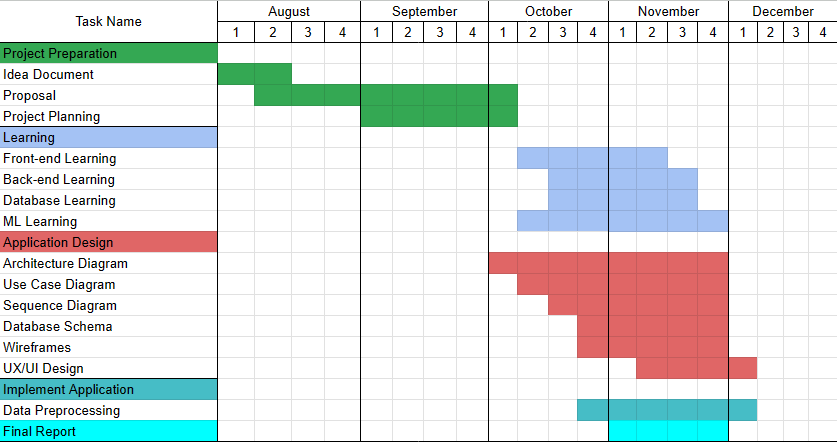
\includegraphics[width=15cm]{./Gantt_Chart_1st_Sem.png}}
  \caption{ภาคการศึกษาที่ 1}\label{fig:Gantt_Chart_1st_Sem}
\end{figure}

\begin{figure}[!h]\centering
  \setlength{\fboxrule}{0.5mm} % can define this in the preamble
  \setlength{\fboxsep}{0.5cm}
  \fbox{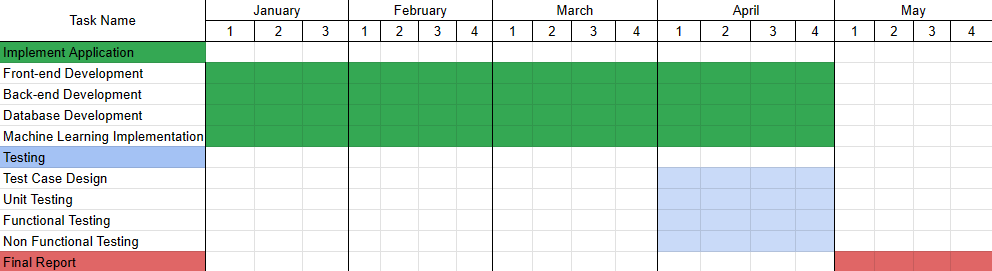
\includegraphics[width=15cm]{./Gantt_Chart_2nd_Sem.png}}
  \caption{ภาคการศึกษาที่ 2}\label{fig:Gantt_Chart_2nd_Sem}
\end{figure}

\newpage
\section{ขอบเขตของโครงงาน}
แอปพลิเคชันสำหรับการแนะนำกิจกรรม และชมรมให้แก่นักศึกษา โดยมีขีดความสามารถดังต่อไปนี้

\begin{enumerate}
  \item ระบบ Log in ผ่านอีเมลของมหาวิทยาลัย \\
  \item ระบบรวบรวมข้อมูลของชมรมต่าง ๆ เอาไว้ โดยผู้ใช้สามารถค้นหาและติดตามข้อมูลของชมรมที่ตนเองสนใจได้ \\
  \item ระบบแจ้งเตือนกิจกรรมที่เกี่ยวข้องกับชมรมหรือความสนใจของนักศึกษา \\
  \item ระบบแจ้งเตือนการประเมินผลกิจกรรม เมื่อฟอร์มการประเมินพร้อมใช้งาน \\
  \item ระบบแนะนำกิจกรรมและชมรม ตามความสนใจของผู้ใช้โดยอ้างอิงจาก tag ของกิจกรรม \\
  \item ระบบวิเคราะห์ความสนใจของผู้ใช้ผ่านเนื้อหาของกิจกรรมที่ผู้ใช้เคยเข้าร่วม เข้าไปอ่านรายละเอียด หรือเกี่ยวข้องกับชมรมที่สนใจ \\
  \item ระบบแยกประเภทกิจกรรมอัตโนมัติโดยวิเคราะห์จากเนื้อหา ออกมาเป็น tag ต่าง ๆ โดยใช้ Machine Learning \\
\end{enumerate}

\section{ประโยชน์ที่คาดว่าจะได้่รับ}

1. แอปพลิเคชันที่สนับสนุนการเข้าร่วมกิจกรรมของนักศึกษา และสามารถแนะนำ กิจกรรม ชมรมที่นักศึกษาน่าจะสนใจได้ \\
2. การจำแนกประเภทของกิจกรรมของนักศึกษา \\

%%%%%%%%%%%%%%%%%%%%%%%%%%%%%%%%%%%%%%%%%%%%%%%%%%%%%%%%%%%%
%%%%%%%%%%%%%%  Literature Review %%%%%%%%%%%%%%%%%%%%%%%%%%
%%%%%%%%%%%%%%%%%%%%%%%%%%%%%%%%%%%%%%%%%%%%%%%%%%%%%%%%%%%%
\chapter{ทฤษฎีความรู้และงานที่เกี่ยวข้อง}
รายละเอียดของทฤษฏี ความรู้ และเทคโนโลยีที่นำมาใช้ในการสร้างและพัฒนาแอปพลิเคชัน

\section{ทฤษฏีและความรู้ที่เกี่ยวข้อง}
  \subsection {Machine Learning}
  \subsubsection {Content-Based Filtering}
Content-Based Filtering เป็นหนึ่งในแนวทางที่ได้รับความนิยมอย่างมากในระบบการแนะนำ เนื่องจากความสามารถในการให้คำแนะนำที่มีความเป็นบุคคลและเกี่ยวข้องกับความสนใจของผู้ใช้งาน 
กระบวนการนี้เน้นการวิเคราะห์เนื้อหาที่ผู้ใช้งานมีความสนใจและแนะนำสิ่งที่มีเนื้อหาที่คล้ายคลึงกันให้กับผู้ใช้งาน ตัวอย่างเช่น การแนะนำหนังสือที่มีเนื้อหาใกล้เคียงกับที่ผู้ใช้งานเคยซื้อมาก่อนหน้านี้ 
ดังนั้นเทคนิคนี้จึงเป็นการสร้างคำแนะนำที่เน้นความเป็นบุคคลและความสอดคล้องกับความต้องการของผู้ใช้งานอย่างมีความแม่นยำและเหมาะสม 
อย่างไรก็ตามการทำ Content-Based Filtering นั้น จะยึดตามความสนใจของผู้ใช้งานที่มีประวัติเก็บเอาไว้ทำให้สามารถแนะนำได้ในวงแคบ ๆ เท่านั้น
\subsubsection {Collaborative Filtering}
  Collaborative Filtering เป็นหนึ่งในแนวทางที่ได้รับความนิยมอย่างมากในการสร้างคำแนะนำสำหรับผู้ใช้งาน แนวทางนี้เสนอหลักการแนะนำที่มาจากพฤติกรรมการใช้งานที่เกิดขึ้นก่อนหน้านี้ของผู้ใช้งาน 
  การ Collaborative Filtering มีวิธีการหลักที่สำคัญสองวิธีคือ \\
  User-Based Collaborative Filtering: แนวทางนี้จะทำการแนะนำสิ่งที่ผู้ใช้งานมีความสนใจอยู่ หากมีความคล้ายคลึงในพฤติกรรมการใช้งานระหว่างผู้ใช้งานสองคน 
  เช่น ถ้าผู้ใช้งานสองคนมีรูปแบบพฤติกรรมที่คล้ายกัน ระบบจะแนะนำสิ่งที่ผู้ใช้อีกคนเคยใช้งานให้กับผู้ใช้งานคนอื่น ซึ่งเพิ่มโอกาสที่จะให้คำแนะนำที่หลากหลายขึ้นได้ 
  อย่างไรก็ตามก็อาจมีโกาสที่จะแนะนำสิ่งที่ผู้ใช้งานไม่สนใจเลยได้เช่นกัน และยังมีปัญหาความซับซ้อนเกิดขึ้นได้หากมีผู้ใช้งานหรือสิ่งที่จะแนะนำเป็นจำนวนมาก \\
  Item-Based Collaborative Filtering: แนวทางนี้จะทำการแนะนำสิ่งที่ผู้ใช้งานมีความสนใจ และจะทำการแนะนำสิ่งที่มีเนื้อหาคล้ายกัน เมื่อพิจารณาการกระทำที่เกิดขึ้นก่อนหน้านี้ 
  ระบบจะแนะนำสิ่งที่มีความคล้ายคลึงให้กับผู้ใช้งาน อย่างไรก็ดีเนื่องจากเป็นการแนะนำจากสิ่งที่มีความใกล้เคียงกัน คำแนะนำที่ได้จึงอาจไม่ใช่สิ่งที่ผู้ใช้งานมองหา \\
\subsubsection {Natural Language Processing \cite{NLP1}, \cite{NLP2}, \cite{NLP3}, \cite{NLP4}, \cite{NLP5}}
Natural Language Processing หรือ NLP เป็นสาขาหนึ่งของปัญญาประดิษฐ์ ที่จะมุ่งเน้นการให้ความสามารถแก่คอมพิวเตอร์ที่เป็นการเข้าใจ ตีความ และปฏิสัมพันธ์กับภาษาของมนุษย์ 
แนวทางนี้นำเอาอัลกอริทึมและเทคนิคในการประมวลผล วิเคราะห์ และสร้างข้อมูลข้อความและเสียง เพื่อให้เครื่องคอมพิวเตอร์สามารถสกัดความหมาย บริบท และความรู้จากภาษาที่มนุษย์สร้างขึ้นได้ \\
  \subsubsection {Word Embedding}
	 Word Embedding ในการทำ Natural Language Processing คือการที่แปลงคำต่าง ๆ ออกมาเป็น vector เพื่อที่จะตรวจสอบความหมายของคำและความหมายในการสร้างประโยค 
   ซึ่งเป็นพื้นฐานในการทำ Natural Language Processing Model ซึ่งสามารถนำมาประยุกต์ได้ทั้งการที่จะจัดประเภทกิจกรรมหรือการวิเคราะห์ความต้องการของผู้ใช้งานจากข้อความที่ถูกใช้ \\

\newpage

   \subsubsection {Transformer Model}
   Transformer Model คือสถาปัตยกรรมการเรียนรู้ของเครื่อง สำหรับการประมวลผลและทำความเข้าใจภาษาของมนุษย์ ซึ่งทำงานได้ดีในการแปลภาษา การสรุป และการสร้างข้อความ 
   โดยอาศัยหลักการของ self-attention ในการทำความเข้าความสัมพันธ์ระหว่างคำในประโยคพร้อมกัน ทำให้สามารถเข้าใจบริบทและความหมายได้มากขึ้นอย่างมีประสิทธิภาพ 
   โดย Transformer-base model ที่ถูกใช้งานในโครงงานนี้ มี 2 รูปแบบ คือ 
   
   \begin{enumerate}
   \item T5 (Text-to-Text Transfer Transformer) เป็นสถาปัตยกรรมที่ประยุกต์มาจาก unified text-to-text framework ซึ่งพัฒนาจาก NLP model หลากหลายงานให้ใช้งานง่ายขึ้น จึงสามารถนำมา train ต่อเพื่อทำงานเกี่ยวกับ Natural language processing ได้อย่างเอนกประสงค์ โดยที่มีผลกระทบต่อประสิทธิภาพในการทำงานเพียงเล็กน้อย อย่างไรก็ตาม T5 มีข้อจำกัดในการเข้าใจบริบทของข้อความและต้องอาศัยการปรับแต่งในการทำงานที่เฉพาะด้าน
   \item BERT (Bidirectional Encoder Representations from Transformers)  สถาปัตยกรรมที่ถูก train โดยคลังข้อความขนาดใหญ่ จึงสามารถทำงานในการจับบริบทที่อยู่เบื้องหลังข้อความได้ เหมาะกับการทำงาน Natural language processing ที่หลากหลาย อย่างไรก็ตาม BERT ต้องการหน่วยประมวลผลในการ train และใช้งาน รวมไปถึงไม่สามารถปรับแต่งได้เอนกประสงค์เท่า T5 
   \end{enumerate} 
   
   \subsubsection {Artificial Neural Network}
   Neural Network เป็นสถาปัตยกรรมการเรียนรู้ของเครื่องที่ได้รับแรงบันดาลใจมาจากระบบประสาทของมนุษย์ โดยมีหลักการคือการแบ่งการทำงานเป็น node ต่าง ๆ 
   ที่รับค่าที่ประมวลผลมาจาก node ที่อยู่ใน input layer แล้วส่งต่อให้ node ประมวลผลที่อยู่ใน hidden layer ไปเรื่อย ๆ จนถึง node ประมวลผลสุดท้ายใน output layer 
   เพื่อตีความผลลัพธ์ ซึ่งสามารถทำงานได้หลากหลายรวมไปถึงงาน Natural Language Processing ซึ่งในโครงงานนี้มี Artifical Neural Network 2  รูปแบบ คือ
   
   \begin{enumerate}
   \item Shallow Neural Network ซึ่งเป็น Neural Network ที่มีจำนวน Layer ในการประมวลผลอยู่น้อย มีข้อดีคือการที่จะใช้หน่วยประมวลผลน้อยและสามารถ train ได้ไว แต่ในทางกลับกันก็มีข้อจำกัดในการตีความที่ซับซ้อนรวมถึงบริบทที่อยู่ในข้อความของงาน Natural Language Processing
   \item Regularizing and Optimizing LSTM Language Model คือ Neural Network ที่ถูกพัฒนามาสำหรับการทำ Natural Language Processing ทำให้สามารถประมวลผลข้อมูลที่มีความต่อเนื่องอย่างเช่นประโยคได้ ตัวโมเดลมีความสามารถในการทำความเข้าใจบริบทในข้อความได้ โดยพิจารณาข้อมูลในหน่วยความจำของโมเดล ซึ่งสามารถจดจำหรือลบข้อมูลได้ตามความเหมาะสม และสามารถรับมือกับข้อความที่ไม่รู้จักได้ดี อย่างไรก็ตามคุณภาพของ model ขึ้นอยู่กับคุณภาพของข้อมูลที่ใช้ train และการปรับแต่งค่อนข้างส่งผลกับตัว model
   \end{enumerate}
   
   \newpage
   \subsection {Mobile App Architecture \cite{MobileAppArchitecture}} 
   ในการพัฒนาแอปพลิเคชัน สถาปัตยกรรมหมายถึงกฎ กระบวนการ และโครงสร้างภายในของแอปพลิเคชัน หรือก็คือวิธีการสร้างแอปพลิเคชัน โดยจะเป็นเรื่องของการกำหนดรูปแบบที่ส่วนประกอบต่าง ๆ สื่อสารกันเพื่อประมวลผลข้อมูล input จากผู้ใช้และประมวลผลข้อมูล output ให้กับผู้ใช้ 

  \begin{figure}[!h]\centering
    \setlength{\fboxrule}{0.5mm} % can define this in the preamble
    \setlength{\fboxsep}{0.5cm}
    \fbox{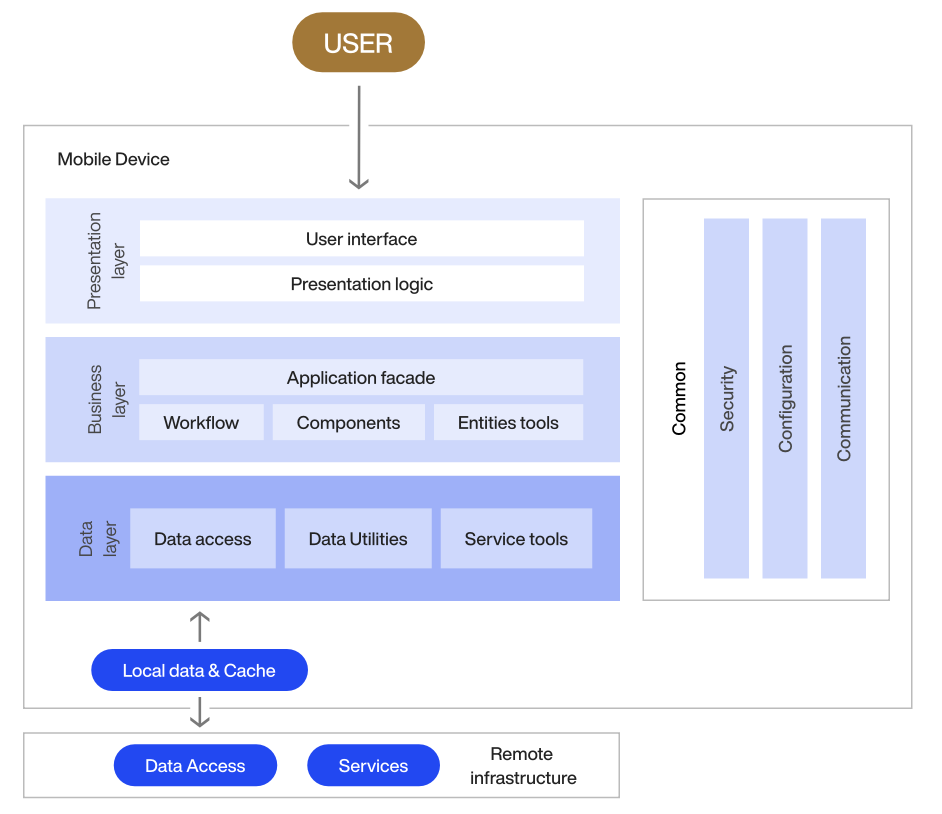
\includegraphics[width=11cm]{./Mobil_Arc.png}}
    \caption{Mobile App Architecture \cite{MobileAppArchitectureOverview}}\label{fig:mobile_arc1}
    \end{figure}

สถาปัตยกรรมของแอปพลิเคชันส่วนใหญ่จะประกอบด้วยสามเลเยอร์หลัก ๆ ได้แก่ Presentation layer, Business layer \cite{BusinessLayer} และ Data layer \\
\begin{enumerate} 
\item Presentation layer \cite{PresentationLayer}
หรือ front end คือส่วนของแอปพลิเคชันที่ผู้ใช้มองเห็นและมีปฏิสัมพันธ์ด้วยได้ โดยมีส่วนติดต่อผู้ใช้ (user interface หรือ UI) ของแอปพลิเคชันเป็นส่วนสำคัญของเลเยอร์นี้
วัตถุประสงค์หลักของเลเยอร์นี้คือการนำข้อมูลที่ส่งมาจาก business layer มาแสดงผลในลักษณะที่ผู้ใช้สามารถเข้าใจได้
ไม่ว่าจะเป็น UI แบบพื้นฐาน เช่น UI แสดงที่อยู่อีเมลของผู้ใช้หรือ UI ที่ซับซ้อน เช่น แอปซื้อขายหุ้นซึ่งแสดงข้อมูลสดเกี่ยวกับตลาดหลักทรัพย์ออกมาแสดงเป็นกราฟหรือแผนภูมิ แม้ว่านักพัฒนาส่วนใหญ่จะรับผิดชอบ Business layer และ Data layer

  \begin{figure}[!h]\centering
    \setlength{\fboxrule}{0.5mm} % can define this in the preamble
    \setlength{\fboxsep}{0.5cm}
    \fbox{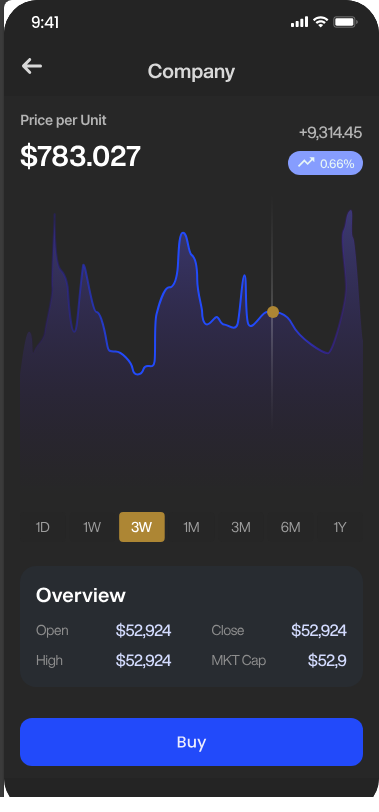
\includegraphics[width=4cm]{./Mobile_Arc2.png}}
    \caption{Presentation layer}\label{fig:mobile_arc2}
    \end{figure}

\newpage
\item Business layer \\
เลเยอร์นี้จะประกอบด้วยตรรกะหลักของแอปพลิเคชัน หรือก็คือวิธีการทำงานของแอปพลิเคชัน โดยมักจะเป็นการนำข้อมูลที่ผู้ใช้ป้อนหรือข้อมูลจาก Data layer มาประมวลผล จากนั้นจึงส่งไปยัง presentation layer
ส่วนใหญ่ business layer จะเป็นส่วนที่ซับซ้อนที่สุดในแอปพลิเคชัน 
โดยปกติแล้วจะแบ่งออกเป็น Layer ย่อยๆหรือส่วนประกอบหลายส่วน โดยแต่ละส่วนมีหน้าที่รับผิดชอบในการทำงานเฉพาะ
ตัวอย่างเช่น หากคุณมีแอปการจัดการทรัพยากรองค์กร (ERP) business layer อาจมีส่วนประกอบสำหรับการจัดการคลังสินค้าและระบบจัดการสินค้าคงคลัง 

  \begin{figure}[!h]\centering
    \setlength{\fboxrule}{0.5mm} % can define this in the preamble
    \setlength{\fboxsep}{0.4cm}
    \fbox{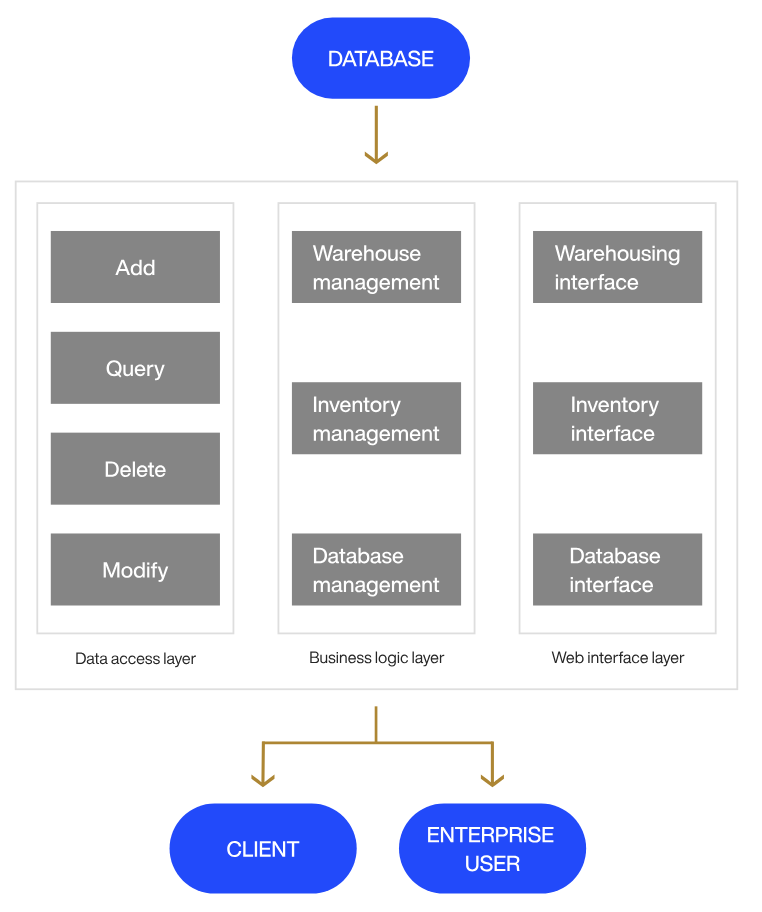
\includegraphics[width=11cm]{./Business_layer.png}}
    \caption{Business layer}\label{fig:business_layer}
    \end{figure}

\newpage
\item Data layer \\
Layer นี้เป็นตัวกลางระหว่าง Layer อื่นๆ กับทรัพยากรภายนอก
วัตถุประสงค์หลักของ Layer นี้คือการรวบรวมข้อมูลจากแหล่งต่างๆ เช่น ฐานข้อมูล, เซิร์ฟเวอร์คลาวด์ หรือ API แล้วส่งไปยัง Layer ด้านบน 
ตัวอย่างเช่น เมื่อผู้ใช้ขอให้แอปพลิเคชันแสดงโปรไฟล์ของตน data layer จะเชื่อมต่อกับ Database และขอข้อมูลที่เกี่ยวข้องทั้งหมด เช่น ชื่อ วันเกิด ไฟล์รูปภาพ และอื่นๆ อย่างไรก็ตามใน layer นี้ข้อมูลส่วนใหญ่ยังไม่ผ่านการประมวลผล จึงอาจจะมีข้อมูลบางอย่าง เช่น แท็กหรือไอดีที่ผู้ใช้ไม่ควรเห็น ในส่วนนี้จึงต้องทำการส่งข้อมูลให้ business layer ประมวลผลเพิ่มเติมเป็นลำดับต่อไป
\end{enumerate}

\newpage

\subsection {HTTP Protocol \cite{HTTPProtocol}} 
\subsubsection {HTTP Protocol คืออะไร}
HTTP (Hypertext Transfer Protocol) เป็นโปรโตคอลที่ใช้ในการแลกเปลี่ยนข้อมูลผ่านทางอินเทอร์เน็ต เปรียบเสมือนระบบส่งข้อมูลบนอินเทอร์เน็ตที่ช่วยให้มั่นใจได้ว่าข้อมูลจะถูกส่งจากที่หนึ่งไปยังอีกที่หนึ่งได้ 
\subsubsection {HTTP Request-Response Cycle \cite{HTTPCycle}}

  \begin{figure}[!h]\centering
    \setlength{\fboxrule}{0.5mm} % can define this in the preamble
    \setlength{\fboxsep}{0.3cm}
    \fbox{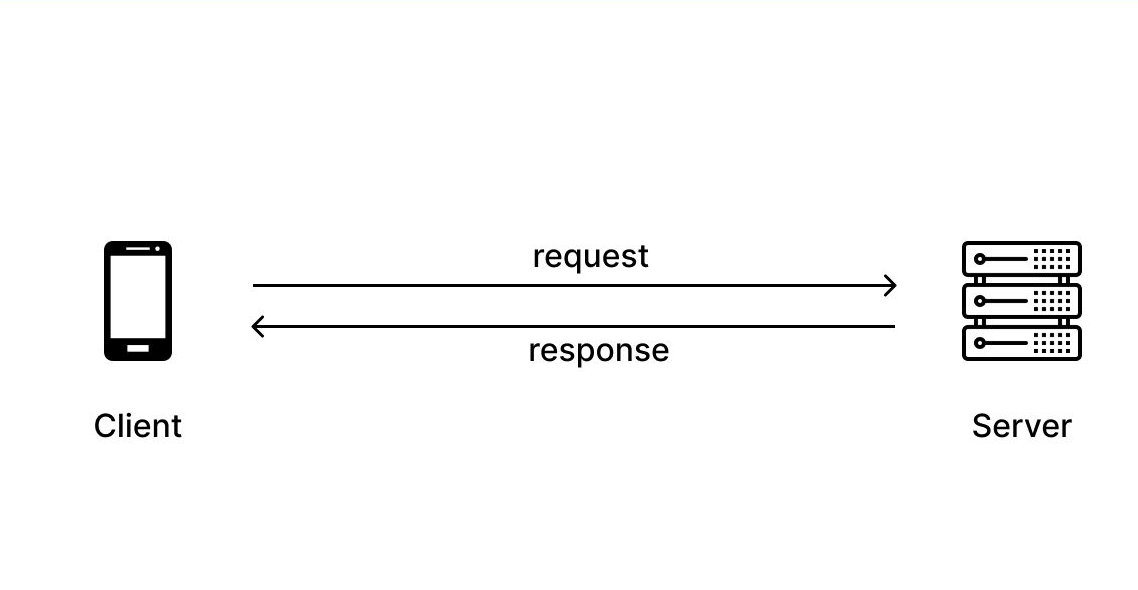
\includegraphics[width=10cm]{./HTTP.png}}
    \caption{HTTP Request-Response Cycle}\label{fig:http}
    \end{figure}

การสื่อสารในโปรโตคอล HTTP มีศูนย์กลางอยู่ที่แนวคิดที่เรียกว่า Request-Response Cycle เป็นกระบวนการที่ไคลเอนต์ (Client) เช่น เว็บเบราว์เซอร์หรือแอปพลิเคชันมือถือ สื่อสารกับเซิร์ฟเวอร์ (Server) เพื่อขอทรัพยากรที่ต้องการหรือเพื่อดำเนินการบางอย่าง โดยวงจรประกอบด้วยหลายขั้นตอนได้แก่ \\
\begin{enumerate}
\item ไคลเอนต์เริ่มต้นการส่งคำขอไปยังเซิร์ฟเวอร์โดยการส่งข้อความร้องขอ (HTTP request message) ซึ่งประกอบด้วยข้อมูลอาทิเช่นทรัพยากรที่ต้องการและพารามิเตอร์เพิ่มเติมอื่น ๆ
\item เซิร์ฟเวอร์ได้รับข้อความร้องขอและประมวลผลโดยใช้ทรัพยากรที่มีอยู่เพื่อสร้างข้อความตอบกลับ (HTTP response message)
\item เซิร์ฟเวอร์ส่งข้อความตอบกลับไปยังไคลเอนต์ ซึ่งโดยทั่วไปจะมีทรัพยากรที่ร้องขอ (เช่น หน้าเว็บ) และข้อมูลเพิ่มเติมหรือเมทาดาตา (ข้อมูลที่ใช้อธิบายชุดข้อมูลอื่นอีกที)
\item ไคลเอนต์ได้รับข้อความตอบกลับและประมวลผล โดยปกติจะเป็นการแสดงเนื้อหาในเว็บเบราว์เซอร์หรือในแอปพลิเคชัน
\item ไคลเอนต์อาจเริ่มการร้องขอเพิ่มเติมไปยังเซิร์ฟเวอร์ โดยทำซ้ำขั้นตอนเดิมแล้วแต่ความจำเป็น
\end{enumerate}

\subsubsection {HTTP Request Methods}
Request method จะเป็นการบอกเซิร์ฟเวอร์ว่าลูกค้าต้องการให้เซิร์ฟเวอร์ดำเนินการอะไร 
Request method ที่พบเจอบ่อยจะมีดังนี้ \\ \\

\begin{table}[]\centering
  \begin{tabular}{|
  >{\columncolor[HTML]{FFFFFF}}c |c|}
  \hline
  \cellcolor[HTML]{6D9EEB}HTTP METHODS & \cellcolor[HTML]{6D9EEB}DEFINITION                \\ \hline
  {\color[HTML]{0A0A23} HEAD} & \cellcolor[HTML]{FFFFFF}ถามเซิร์ฟเวอร์เกี่ยวกับสถานะ (ขนาด ความพร้อมใช้งาน) ของทรัพยากร \\ \hline
  {\color[HTML]{0A0A23} GET}           & ขอทรัพยากรจากเซิร์ฟเวอร์                          \\ \hline
  {\color[HTML]{0A0A23} POST}          & ขอให้เซิร์ฟเวอร์สร้างทรัพยากรใหม่                 \\ \hline
  {\color[HTML]{0A0A23} PUT}           & ขอให้เซิร์ฟเวอร์แก้ไข/อัปเดตทรัพยากรที่มีอยู่แล้ว \\ \hline
  {\color[HTML]{0A0A23} DELETE}        & ขอให้เซิร์ฟเวอร์ลบทรัพยากร                        \\ \hline
  \end{tabular}
    \caption{HTTP Request Methods}\label{tab:HTTP Request Methods}
\end{table}

\FloatBarrier
\subsection {REST API \cite{RestAPI}} 
\subsubsection {REST คืออะไร}
REST ย่อมาจาก Representational State Transfer เป็นรูปแบบการส่งข้อมูลระหว่าง Server-Client รูปแบบหนึ่งซึ่งอยู่บนพื้นฐานของ HTTP Protocol เป็นการสร้าง Web Service เพื่อแลกเปลี่ยนข้อมูลกันผ่าน Application วิธีหนึ่ง ซึ่งส่งข้อมูลได้หลายชนิด ไม่ว่าจะเป็น Text, XML, JSON หรือส่งมาเป็นหน้า HTML เลย
REST ทำงานอยู่บน HTTP Protocol ทำให้เวลาใช้งานจะต้องอยู่บนพื้นฐาน HTTP Method เช่น GET, POST, PUT, DELETE จะใช้ Method ไหนก็ขึ้นอยู่กับว่าจะทำอะไรกับข้อมูล แต่ก็ต้องควรใช้คู่กับ Operation CURD เช่น เมื่อต้องการจะเรียกดูข้อมูลทั้งหมดก็ใช้ GET เมื่อต้องการเพิ่มข้อมูลก็ใช้ POST เป็นต้น \\
\subsubsection {การออกแบบ REST API \cite{RestAPIDesign}}

\begin{enumerate}
  \item เลือกใช้ HTTP Method ให้เหมาะสมกับการใช้งาน
    ในกรณีปกติ การสร้าง URL จะไม่ใส่ชื่อกิริยาของ API มาอยูใน path เช่น /createUsers, /getUserDetail นั้นผิดหลักในการสร้าง เนื่องจากในการที่จะระบุว่าแต่ละ API จะถูกใช้ทำหน้าที่อะไรนั้นจะมี HTTP Method ในการระบุอยู่แล้ว 
  \item การสร้าง URL ของ API endpoint ให้ตรงตามมาตรฐานในการสร้าง URL ของ API นั้นมีทั้งหมดสามกฎที่สำคัญ ก็คือ

  \begin{itemize}
    \item ควรจะมีแค่ชื่อ resource เท่านั้น เนื่องจาก resource เป็นตัวแทนของ สิ่งของบางอย่าง ที่เชื่อมโยงกับข้อมูล เช่น Users, Customers, Orders
    \item ชื่อ path ควรจะเป็นรูปพหูพจน์ของ resource 
    \item ไม่ควรจะมีชื่อกิริยาที่บอกถึงวัตถุประสงค์ของ API (เช่น add, update, delete) ตามที่กล่าวในข้อแรก
  \end{itemize}
สมมติว่าต้องการ API ที่เกี่ยวข้องกับ Users โดยการสามารถ สร้างข้อมูล user, แก้ไขข้อมูล user, แสดงข้อมูล user และ ลบข้อมูล user สามารถเขียนออกมาได้ดังนี้
  \begin{itemize}
    \item method: POST path: /users สร้างข้อมูล user ใหม่
    \item method: PUT path: /users/99 จะแก้ไขข้อมูล user ที่ id 99
    \item method: GET path: /users จะได้ข้อมูลของ user ทั้งหมด
    \item method: GET path: /users/99 จะได้รายละเอียดของ user ที่ id 99
    \item method: DELETE path: /users/99 จะเป็นการลบข้อมูล user ที่ id 99
  \end{itemize}
กรณีที่ข้อมูลความเกี่ยวข้องกัน ส่วนใหญ่จะใช้เป็น Nested endpoint แทน query string เช่น ต้องการข้อมูลของ user ทั้งหมดที่อยู่ใน customer id เป็น 2 สามารถเขียนเป็น GET /customers/2/users 
แต่มีบางกรณีที่ ข้อมูล Nested ที่เยอะมากๆจนหากใช้งานเป็น URL path จะมียาวมากเกินไป อาจจะใส่เป็น query string หรือ ใส่ใน body แทน เพื่อให้อ่านได้ง่ายขึ้น ซึ่งต้องพิจารณาถึง use case ด้วย
  \item ควรมี API Versioning
    หาก API มีผู้ใช้เข้ามาใช้งานแล้ว ในการแก้ไขสิ่งที่มีขนาดใหญ่ ก็จะทำได้ลำบากขึ้น เพราะถ้าแก้ไปแล้ว ทำให้ service ที่ใช้ API อยู่ใช้งานไม่ได้อาจจะทำให้เกิดปัญหาขึ้น เพราะอย่างนั้น ทุก ๆ API ควรทำ version ไว้ หากมีการเปลี่ยนแปลงก็สามารถแยกออกมาเป็นอีก version ได้เลย โดยทั้ง version เก่าและใหม่ต้องทำงานได้ทั้งคู่ ตัวอย่างเช่น
    POST v1/users และ POST v2/users สามารถนำเลข version มาต่อหน้า API ได้เลย
  \item การตั้งชื่อ (Naming Conventions) ให้สัมพันธ์กันทั้งระบบ
    การตั้งชื่อตัวแปร (ของ body และ response) ที่พบเจอบ่อยที่สุดจะเป็น camel case, snake case เป็น key ซึ่งสามารถเลือกใช้ได้ตามใจชอบ แต่ควรตั้งชื่อให้เหมือนกันทั้งระบบ
    \item ใช้งาน parameters ให้เหมาะสม
    parameters คือ query ที่ต่อท้าย URL path ซึ่งจะมี action ต่างๆ ดังนี้
  \begin{itemize}
    \item Filtering (การกรองข้อมูล) สามารถกรองข้อมูลแบบมีเงื่อนไขได้ โดย จะส่งผ่านมาทาง query ที่ต่อท้าย URL path เช่น GET /orders?name=MyOrders\&customerId=2
      ผลลัพธ์หลัง filter คือข้อมูลของ order ที่มีชื่อว่า “MyOrders” และอยู่ใน customer id ที่ 2 จากหลักการข้อ 2. ที่กล่าวไปว่า ข้อมูล Nested ที่เยอะมาก ๆ หรือต้องการกรองข้อมูลจำนวนมาก ถ้าเอามาเป็น URL path จะมีความยาวเกินไป สามารถนำมาใส่ใน filter ต่อท้าย URL path แทนได้ \\ 
    \item Sorting (การจัดเรียงข้อมูล) สามารถเรียงลำดับข้อมูลที่เรียกมาแสดงผลได้ ซึ่งการออกแบบ sort ที่ดีจะต้องออกแบบให้ยืดหยุ่น สามารถเรียงจากน้อยไปมาก หรือมากไปน้อยได้ โดยใส่ query เข้าไปต่อท้าย path คล้ายกับ filter ซึ่งสามารถนำ sort by ไปต่อท้ายได้ เช่น
      GET /users?sort by=+email หรือ GET /users?sort by=-email
จากตัวอย่างด้านบน +email คือการเรียงจากน้อยไปมาก และ -email เรียงจากมากไปน้อย หรือสามารถเขียนในรูปแบบอื่นๆ ได้เช่น
    \item GET /users?sort by=asc(email) หรือ GET /users?sort by=desc(email)
    \item GET /users?sort by=email.asc หรือ GET /users?sort by=email.desc
    \item GET /users?sort by=email\&order by=asc หรือ GET /users?sort by=email\&order by=desc
  \end{itemize}
โดยหลักสำคัญจะอยู่ที่ทุกรูปแบบการเขียนจะต้องหยืดหยุ่น สามารถเปลี่ยนลำดับการเรียงข้อมูลได้ และผู้ใช้งานสามารถอ่านได้อย่างเข้าใจว่าเป็นการเรียงลำดับแบบไหน \\
  \begin{itemize} 
    \item Searching (การค้นหาข้อมูล) หลักการจะค่อนข้างคล้าย filter คือการค้นหาข้อมูลแบบมีเงื่อนไข เมื่อต้องการค้นหาข้อมูล จะส่งผ่านมาทาง query ต่อท้าย String ตัวอย่างเช่น เมื่อต้องการค้นหาชื่อของ order ที่ชื่อว่า “THAIPOST1234” ในระบบ จะส่งผ่านทาง query params ตามตัวอย่างด้านล่าง
      GET /orders?search='THAIPOST1234' \\ 
    \item Pagination (การจัดแบ่งหน้า) \cite{Pagination} สามารถจัดหน้าของข้อมูลได้ในกรณีที่ข้อมูลมีจำนวนมาก
  \end{itemize}
    \begin{figure}[!h]\centering
      \setlength{\fboxrule}{0.5mm} % can define this in the preamble
      \setlength{\fboxsep}{0.5cm}
      \fbox{
\includegraphics[width=10cm]{./google.png}}
      \caption{tab เลือกหน้าของ Google}\label{fig:google}
    \end{figure}
ตัว paginate จะช่วยย่อยข้อมูลออกมาเป็นก้อนเล็ก ๆ โดยสามารถโยน query เพื่อระบุหน้า จำนวนข้อมูลที่ต้องการแสดงได้ เช่น GET /orders?page=2\&limit=50
ผลลัพธ์ที่ได้จะเป็นข้อมูลตัวที่ 51–100 นั้นเอง เพราะเป็น page ที่ 2 ข้อมูลจำนวน 50 ตัว \\

\newpage

  \item ใช้ HTTP Status code ให้ตรงตามความหมาย
    หลังจากที่ฝั่งผู้ใช้งาน API (Client) ส่ง request ไปหา server ผ่าน API แล้วฝั่ง Client จะต้องทำการยืนยันให้ได้ว่า API ใช้งานได้จริงหรือไม่ หรือส่งไปสำเร็จไหม จึงมีการต้องส่ง response ที่มี HTTP Status code ระบุ กลับไปยัง client เพื่อบอกว่า request นั้น ๆ Pass, Fail หรือ request นั้นผิด
    กรณี Success จะมี HTTP status code ที่ใช้งานกันทั่วไปได้แก่ 
  \begin{itemize}
    \item  200 Ok: เป็นมาตรฐานของ HTTP response เพื่อบ่งบอกว่า request นั้นสำเร็จ ใช้สำหรับ GET, PUT หรือ POST ก็ได้
    \item 201 Created: เป็น response เพื่อบ่งบอกว่าข้อมูลใหม่ได้ถูกสร้างขึ้นสำเร็จ ใช้สำหรับ POST
    \item 204 No Content: เป็น response สำหรับบ่งบอกดำเนินการ Success แต่ไม่ได้ return ข้อมูลกลับ ส่วนใหญ่จะใช้กรณีลบข้อมูล DELETE ที่ไม่ได้ส่ง response ที่เป็นข้อมูลกลับไป
      กรณี Error จะมี HTTP status code ที่ใช้งานกันทั่วไปได้แก่
    \item 400 Bad Request: status นี้จะบ่งบอกว่า request ที่ส่งมาโดย client นั้นไม่มี action ใดๆ และ Server ไม่เข้าใจ เช่น JSON ผิด หรือ parameters ไม่ถูกต้อง
    \item 401 Unauthorized: เป็น response ที่บ่งบอกว่า client ไม่ได้รับอนุญาตในการเข้าถึง อาจจะเป็นกรณีที่ใส่ token ผิด หมดอายุ หรือไม่ได้แนบ token มา
    \item 403 Forbidden: เป็น response ที่บ่งบอกว่า client ได้รับการอนุญาตในการเข้าถึงระบบ (login ผ่าน) แต่จะมีข้อมูลบางหน้า ที่ไม่มีสิทธิ์ในการเข้าถึง
    \item 404 Not Found: เป็น response ที่บ่งบอกว่า request นั้นไม่ว่างใช้งานตอนนี้ หรือ request ที่เรียกนั้นไม่มีอยู่ในระบบ
    \item 405 Gone: เป็น response ที่บ่งบอกว่า resource ที่ต้องการนั้นไม่มี หรือถูกย้ายไป
    \item 429 Too many Request: เป็น response ที่บ่งบอกว่า request นั้นติด limit ใช้กรณีที่กำหนด rate limit ไว้ว่า API นั้น ๆ จะสามารถเรียกได้กี่ครั้ง
    \item 500 Internal Server Error: เป็น response ที่บ่งบอกว่าการ request นั้นถูกต้องแล้ว แต่ server พังเอง ซึ่งอาจจะพังที่ตัวโค้ดของระบบเอง
    \item 503 Service Unavailable: เป็น response ที่บ่งบอกว่า server ใช้การไม่ได้ (ระบบพัง) โดย Server จะไม่สามารถรับ request ที่ส่งเข้ามาได้
    \item 504 Bad Gateway Gateway Timeout: เป็น response ที่บ่งบอกว่า web server อย่างพวก nginx หรือ apache พัง
      จะเห็นว่า HTTP Status code แต่ละตัวจะมีความหมายของของตัวเองชัดเจน เพราะฉะนั้นการออกแบบที่ดีจะต้องเลือกให้ HTTP Status code ให้ตรงตามวัตถุประสงค์เพื่อให้ผู้ใช้งานที่ได้รับ response กลับไป เข้าใจ response นั้นได้ดีมากขึ้น \\
  \end{itemize}
  \item การ Handle Error ให้ user เข้าใจ
    นอกเหนือจาก HTTP Status code แล้ว ต้องออกแบบ response สำหรับ error กรณีต่าง ๆ ไว้ด้วย เพื่อให้ user เข้าใจ error ของ API มากขึ้น ยกตัวอย่างกรณีที่ request ส่งบาง parameter มาไม่ถูกต้อง แทนที่จะ response กลับไปว่า
\end{enumerate}

\begin{figure}[!h]\centering
  \setlength{\fboxrule}{0.5mm} % can define this in the preamble
  \setlength{\fboxsep}{0.5cm}
  \fbox{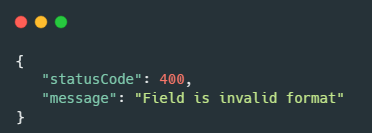
\includegraphics[width=9cm]{./Error1.png}}
  \caption{Handle Error1}\label{fig:Error1}
\end{figure}

ซึ่ง User จะไม่สามารถระบุได้ว่า field ใดที่ผิด format บ้าง

\newpage
\begin{figure}[!h]\centering
  \setlength{\fboxrule}{0.5mm} % can define this in the preamble
  \setlength{\fboxsep}{0.5cm}
  \fbox{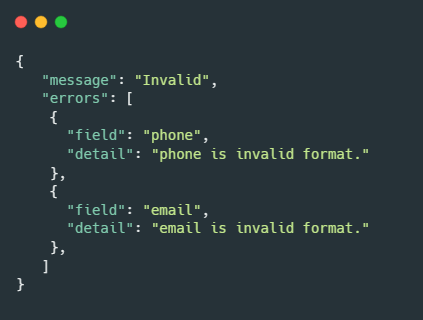
\includegraphics[width=10cm]{./Error2.png}}
  \caption{Handle Error2}\label{fig:Error2}
\end{figure}

การส่งไปในรูปแบบดังกล่าวจะทำให้ user เข้าใจได้เลยว่ามี field ใดที่ผิด format

\subsection {Graph Database \cite{GraphDatabase}} 
\subsubsection {Graph Database คืออะไร}
  Graph database หรือฐานข้อมูลแบบกราฟ จัดเป็น NoSQL Database รูปแบบหนึ่ง ซึ่งนำมาใช้แก้ปัญหา database ที่มีข้อมูลขนาดใหญ่และไม่มีรูปแบบชัดเจน
  ฐานข้อมูลแบบ Graph ออกแบบมาเพื่อแสดงความสัมพันธ์ (Relationship) ระหว่างข้อมูลที่มีความเชื่อมโยงกับข้อมูลที่เราสนใจได้อย่างชัดเจน รวมถึงมีความสามารถในการเก็บข้อมูลที่ไม่ต้องกำหนดรูปแบบล่วงหน้า
\subsubsection {ทำไมต้องเป็น Graph Database}
  การเข้าถึง node และ relationships ในฐานข้อมูล Graph เป็นวิธีที่มีประสิทธิภาพและใช้เวลาในการทำงานคงที่ และช่วยให้เราสำรวจการเชื่อมต่อหลายล้านต่อวินาทีต่อเรคคอร์ดได้อย่างรวดเร็ว
  มีความเป็นอิสระจากขนาดรวมของชุดข้อมูลทั้งหมดของเรา ทำให้ฐานข้อมูลแบบ Graph มีความสามารถในการจัดการข้อมูลที่มีรูปแบบซับซ้อนและมีความเชื่อมต่อกันสูงได้มีประสิทธิภาพ \\
  
\newpage

\subsubsection {Property ของ Graph Model \cite{GraphDatabaseProperty}} 
  เทคโนโลยีส่วนใหญ่มีวิธีการที่แตกต่างกันเล็กน้อยในการสร้าง องค์ประกอบที่สำคัญของฐานข้อมูล Graph วิธีหนึ่ง คือ Graph Model ข้อมูลจะถูกจัดระเบียบเป็น node, relationship และ properties(ข้อมูลที่อยู่บน node หรือ relationship)

  \begin{figure}[!h]\centering
    \setlength{\fboxrule}{0.5mm} % can define this in the preamble
    \setlength{\fboxsep}{0.5cm}
    \fbox{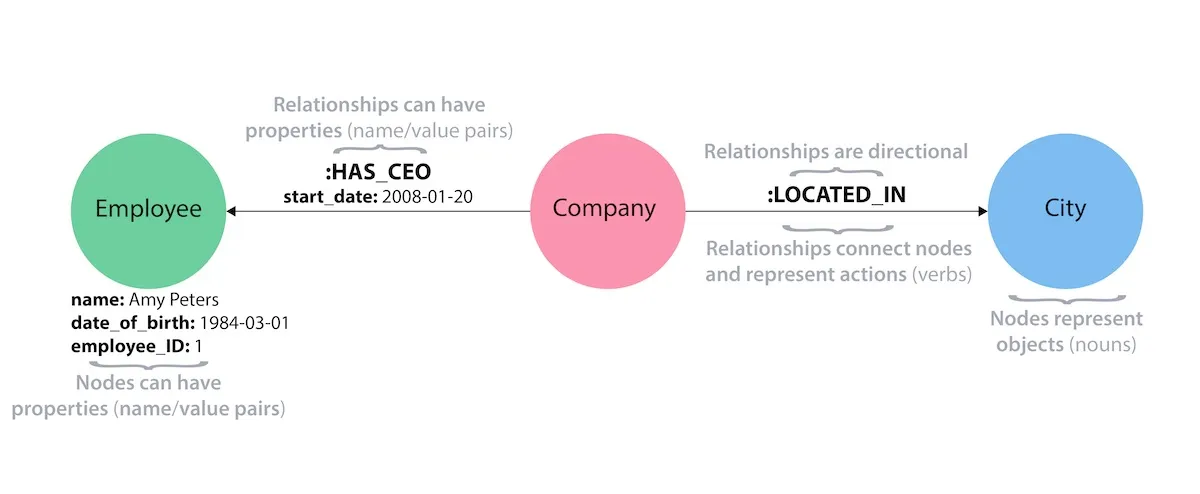
\includegraphics[width=10cm]{./Property.png}}
    \caption{Property ของ Graph Model}\label{fig:Graph}
  \end{figure}

Nodes เป็นเหมือน entity ของ Graph สามารถที่จะเก็บ attribute จำนวนมากได้ สำหรับ Graph เราจะเรียก attribute ว่า properties
Relationships เป็นความสัมพันธ์ที่เชื่อมระหว่าง 2 node และเหมือนกับ node มันสามารถเก็บ properties ได้ \\
\newpage
\subsubsection {Graph Database vs Relational Database \cite{DatabaseCompare}} 

\begin{table}[]
  \begin{tabular}{|c|c|c|}
  \hline
  \rowcolor[HTML]{6D9EEB} 
   &
    {\color[HTML]{242424} Relational Database} &
    \cellcolor[HTML]{93C47D}{\color[HTML]{242424} Graph Database} \\ \hline
  \cellcolor[HTML]{FFFFFF}{\color[HTML]{242424} รูปแบบการเก็บข้อมูล} &
    \cellcolor[HTML]{FFFFFF}{\color[HTML]{242424} ตารางที่มีแถวและคอลัมน์} &
    {\color[HTML]{242424} \begin{tabular}[c]{@{}c@{}}โหนดที่เชื่อมต่อถึงกันพร้อมข้อมูล\\ ที่แสดงเป็นเอกสาร JSON\end{tabular}} \\ \hline
  \cellcolor[HTML]{FFFFFF}{\color[HTML]{242424} การทำงาน} &
    {\color[HTML]{242424} \begin{tabular}[c]{@{}c@{}}การทำงานของ SQL เช่น สร้าง อ่าน \\ อัปเดต และลบ (CRUD)\end{tabular}} &
    {\color[HTML]{242424} \begin{tabular}[c]{@{}c@{}}การดำเนินการรวมถึง CRUD \\ และการดำเนินการผ่านกราฟ\\ ตามทฤษฎีกราฟทางคณิตศาสตร์\end{tabular}} \\ \hline
  \cellcolor[HTML]{FFFFFF}{\color[HTML]{242424} \begin{tabular}[c]{@{}c@{}}ความสามารถ\\ ในการปรับขนาด\end{tabular}} &
    {\color[HTML]{242424} \begin{tabular}[c]{@{}c@{}}ฐานข้อมูลแบบเชิงสัมพันธ์แบบดั้งเดิม\\ สามารถปรับขนาดในแนวตั้งได้\\ แต่ไม่ค่อยเชี่ยวชาญกับการปรับขนาดในแนวนอน\end{tabular}} &
    {\color[HTML]{242424} \begin{tabular}[c]{@{}c@{}}ฐานข้อมูลแบบกราฟเชี่ยวชาญ\\ ในการปรับขนาดตามแนวนอน \\ สามารถใช้การแบ่งพาร์ติชันเพื่อกระจาย\\ ข้อมูลไปยังโหนดจำนวนมาก\end{tabular}} \\ \hline
  {\color[HTML]{242424} ประสิทธิภาพ} &
    {\color[HTML]{242424} \begin{tabular}[c]{@{}c@{}}ฐานข้อมูลแบบเชิงสัมพันธ์เผชิญกับ\\ การสืบค้นที่ซับซ้อนเมื่อสำรวจความสัมพันธ์ที่อาจ\\ ทำให้ประสิทธิภาพการทำงานช้าลง\end{tabular}} &
    {\color[HTML]{242424} \begin{tabular}[c]{@{}c@{}}ฐานข้อมูลแบบกราฟเชี่ยวชาญในการแสดง\\ และสืบค้นความสัมพันธ์ระหว่างข้อมูล\end{tabular}} \\ \hline
  {\color[HTML]{242424} \begin{tabular}[c]{@{}c@{}}ความสะดวก\\ ในการใช้งาน\end{tabular}} &
    {\color[HTML]{242424} \begin{tabular}[c]{@{}c@{}}ฐานข้อมูลแบบเชิงสัมพันธ์ทำงานได้ดีกับ\\ ชุดข้อมูลขนาดใหญ่และข้อมูลที่มีโครงสร้าง \\ พวกมันไม่ค่อยเชี่ยวชาญเมื่อเป็นเรื่อง\\ การสืบค้นแบบหลายช่วง\end{tabular}} &
    {\color[HTML]{242424} \begin{tabular}[c]{@{}c@{}}ฐานข้อมูลแบบกราฟใช้งานง่าย\\ เมื่อต้องจัดการกับข้อมูลที่เน้นความสัมพันธ์เป็นหลัก \\ เมื่อใช้ภาษาสืบค้นแบบกราฟ \\ คุณสามารถสืบค้นข้อมูลฮอป\\ หลายรายการได้อย่างรวดเร็ว\end{tabular}} \\ \hline
  \end{tabular}
  \caption{\centering Graph Database vs Relational Database}\label{tab:Graph Database vs Relational Database}
  \end{table}

\newpage

\subsection{UML Diagram \cite{UML}} 
\subsubsection{UML Diagram คืออะไร}
UML Diagram คือ แผนภาพที่ใช้ในการแสดงและอธิบายโครงสร้างและพฤติกรรมของ code เพื่อสื่อสารให้ Developer และผู้ที่เกี่ยวข้องทุกคนเข้าใจตรงกัน ซึ่งสามารถเอามาใช้อธิบายความสัมพันธ์ของสิ่งต่างๆที่อยู่ในชิ้นงานได้ โดย UML Diagram มีแผนภาพหลายรูปแบบสำหรับใช้อธิบายโครงสร้างและความสัมพันธ์ในรูปแบบต่างๆที่ Developer ต้องทำความเข้าใจเพื่อใช้ในการปฏิบัติงาน
\subsubsection{Use case Diagram}
Use Case Diagram เป็นหนึ่งใน UML Diagram ที่ใช้ในการแสดงภาพรวมของวิธีการใช้ระบบหรือซอฟต์แวร์ จากมุมมองของผู้ใช้หรือแต่ละกลุ่มผู้ใช้ โดยทำให้ง่ายต่อการเข้าใจและสื่อสารความต้องการของระบบกับผู้ใช้และทีมพัฒนา
ลักษณะหลักของ Use Case Diagram ประกอบด้วย
\begin{enumerate}
  \item Actor : แสดงตัวบุคคลหรือระบบที่มีส่วนร่วมในการใช้งานระบบ สามารถเป็นบุคคล, ระบบภายนอก, หรือภายในระบบได้
  \item Use Case : แสดงกิจกรรมหรือฟังก์ชันที่ระบบหรือซอฟต์แวร์ให้บริการในแต่ละคำสั่งหรือเหตุการณ์ที่มีผู้ใช้ร้องขอ
  \item Association : แสดงความสัมพันธ์ระหว่างผู้เกี่ยวข้องกับ Use Case
  \item System Boundary : แสดงขอบเขตของระบบที่กำหนดไว้ใน Use Case Diagram
  \item Include Relationship : แสดงว่า Use Case หนึ่งสามารถเรียกใช้ (include) Use Case อื่น ๆ ในทำนองของการนำเข้า (include)
  \item Extend Relationship : แสดงว่า Use Case นึงสามารถขยาย (extend) ไปยัง Use Case อื่น ๆ ในกรณีที่มีเหตุการณ์เฉพาะที่เกิดขึ้น
\end{enumerate}
  Use Case Diagram มีประโยชน์มากในการทำความเข้าใจและกำหนดความต้องการของระบบจากมุมมองของผู้ใช้ และช่วยให้ทีมพัฒนามีภาพรวมของฟังก์ชันและการทำงานของระบบที่ชัดเจน\\
\subsubsection{Sequence Diagram}
  Sequence Diagram เป็นหนึ่งใน UML Diagram ที่ใช้งานเพื่อแสดงลำดับขั้นตอนหรือการทำงานของวัตถุต่าง ๆ ภายในระบบหรือโปรแกรม ในแต่ละขั้นตอนของการทำงานนั้นๆ
  ลักษณะหลักของ Sequence Diagram ประกอบด้วย

\begin{enumerate}
  \item Lifeline : แสดงสิ่งต่าง ๆ ที่มีบทบาทในกระบวนการ สามารถเป็นวัตถุ, คลาส, หรือนักพัฒนา
  \item Message : แสดงการสื่อสารระหว่าง Lifeline สามารถแบ่งเป็น Synchronous (ทำงานพร้อมกัน) หรือ Asynchronous (ทำงานไม่พร้อมกัน)
  \item Activation Box : แสดงช่วงเวลาที่วัตถุทำงาน หรือทำการเรียกใช้งาน
  \item Return Message : แสดงการส่งคืนจากการทำงานหรือเรียกใช้งาน
  \item Focus of Control : แสดงว่าในขณะที่โปรแกรมทำงาน, ควบคุมอยู่ที่วัตถุหรือเส้นชีวิตใด
\end{enumerate}
%\subsection{UX/UI Design}



\section{เทคโนโลยี}
\subsection{Integrated Development Environment (IDE)}
\begin{itemize}
  \item Visual Studio Code \cite{VSCode} \\ 
    โปรแกรมสำหรับเขียนโค้ดที่ใช้ในการแก้ไขและปรับแต่งโค้ด จากค่ายไมโครซอฟท์ มีการพัฒนาออกมาในรูปแบบของ OpenSource จึงสามารถนำมาใช้งานได้แบบฟรี ๆ สนับสนุนภาษาโปรแกรมมิ่งมากมายทั้งภาษา JavaScript, TypeScript และ Node.js สามารถเชื่อมต่อกับ Git ได้ นำมาใช้งานได้ง่ายไม่ซับซ้อน มีเครื่องมือส่วนขยายต่าง ๆ ให้เลือกใช้อย่างมากมาย
  \item Pycharm \cite{Pycharm} \\ 
    โปรแกรมสำหรับเขียนโค้ดสำหรับภาษาไพทอน ติดตั้งบนเครื่องคอมพิวเตอร์ ได้ทั้งบนระบบปฏิบัติการ Windows, MacOS และ Linux 
  \item Google Colab \cite{Colab} \\ 
    โปรแกรมสำหรับเขียนโค้ดสำหรับภาษาไพทอนในเบราว์เซอร์ โดยไม่ต้องกำหนดค่าใดและสามารถเข้าถึง GPU โดยไม่มีค่าใช้จ่าย
\end{itemize}
\subsection{Design}
\begin{itemize}
  \item Figma \cite{Figma} \\ 
    เครื่องมือออกแบบ User interface โดยสามารถใช้ออกแบบได้ตั้งแต่เว็บไซต์ แอปพลิเคชัน หรือโลโก้ ในรูปแบบที่มีลูกเล่นมากกว่าที่เคยเห็นในอดีต เช่น การออกแบบ Interactive component เป็นต้น
  \item LucidChart \cite{Lucidchart} \\ 
    เว็บแอปพลิเคชันสำหรับสร้างไดอะแกรม ผังงาน แผนภาพแบบจำลอง หรือแผนที่ความคิด สามารถแชร์แผนภาพให้ผู้อื่นเพื่อทำงานร่วมกันแบบเรียลไทม์ได้ มีเทมเพลตสำเร็จรูปให้เลือกใช้งานได้หลากหลายรูปแบบ เช่น ผังงาน แบบโครงร่าง แผนภาพเครือข่าย และแผนผังเว็บไซต์ เป็นต้น นอกจากนี้ยังสามารถแสดงความคิดเห็น หรือสนทนาแบบกลุ่มได้ และยังดาวน์โหลดเป็นไฟล์รูปแบบต่าง ๆ ได้
\end{itemize}
\subsection{Frontend}
\begin{itemize}
  \item React Native \cite{ReactNative} \\ 
    Cross-Platform Framework ที่ใช้ในการพัฒนา Native Mobile Application สำหรับ Android และ iOS ที่พัฒนาโดยบริษัท Facebook Inc. 
  React Native มีหลักการคล้ายกับ Xamarin คือสามารถ Reuse Code ได้มากกว่า 70% ในการทำแอปพลิเคชันที่รันได้ทั้งบน Android และ iOS โดยใช้ภาษาหลักคือภาษา Javascript และ Typescript ในการพัฒนาแอปพลิเคชัน ซึ่งเมื่อทำเสร็จแอปพลิเคชันจะทำงานไวใกล้เคียงกับการเขียนด้วย ภาษา Native อย่าง Java และ Swift/Objective-C อีกหนึ่งจุดเด่นของ React Native คือการประยุกต์ใช้แนวคิดแบบ Reactive Programming ที่ทำให้การพัฒนารองรับการทำงานแบบ Asynchronous และมี State ที่ซับซ้อนได้
\end{itemize}
\subsection{Backend}
\begin{itemize}
  \item FastAPI \cite{FastAPI} \\ 
    FastAPI คือเว็บเฟรมเวิร์กที่มีความรวดเร็วและประสิทธิภาพสูง สำหรับการสร้าง API ด้วยภาษา Python ที่มีจุดเด่นได้แก่
    1.มีความรวดเร็ว ประสิทธิภาพเทียบเท่ากับ NodeJS และ Go 
    2.สร้างง่าย เพิ่มความเร็วในการพัฒนา
    3.ลดข้อผิดพลาดที่เกิดจากมนุษย์ (นักพัฒนา)
\end{itemize}
\subsection{Database}
\begin{itemize}
  \item Neo4j \cite{Neo4j} \\ 
    เป็นระบบฐานข้อมูลที่ถูกออกแบบมาเพื่อจัดเก็บข้อมูลแบบกราฟ (Graph Database) ที่สามารถจัดเก็บแมปและสอบถามความสัมพันธ์ระหว่างข้อมูลได้อย่างมีประสิทธิภาพและมีความยืดหยุ่น ระบบฐานข้อมูลกราฟนี้ถูกออกแบบมาเพื่อเก็บข้อมูลในรูปแบบของ Node และ เชื่อมต่อระหว่างโหนดด้วยเส้นเชื่อมที่เรียกว่า Relationships ทำให้สามารถแสดงความสัมพันธ์และการเชื่อมโยงของข้อมูลได้อย่างชัดเจน
\end{itemize}
\subsection{Machine Learning}
\begin{itemize}
  \item mT5 \\
    เป็นโมเดลการเรียนรู้ของเครื่องสำหรับการประมวลภาษาธรรมชาติที่มีความหลากหลายในการรับรองภาษาต่าง  ๆ ซึ่งถูกพัฒนาโดย Google Research และเป็นการปรับปรุงจากโมเดล T5 (Text-to-Text Transfer Transformer) ซึ่งเป็นโมเดลที่มีความสามารถในการเรียนรู้จากข้อมูลข้อความและการประมวลผลข้อความอย่างมีประสิทธิภาพ
  \item BERT-th \\
    เป็นโมเดลการเรียนรู้ของเครื่องสำหรับการประมวลภาษาธรรมชาติที่ถูกพัฒนาขึ้นเพื่อใช้ในภาษาไทย โมเดลนี้มีความสามารถในการเข้าใจและประมวลผลข้อมูลที่เป็นภาษาไทยอย่างมีประสิทธิภาพ โดยใช้หลักการของ BERT (Bidirectional Encoder Representations from Transformers) ซึ่งเป็นโมเดลการเรียนรู้ของเครื่องที่สามารถทำนายคำถัดไปในประโยคจากข้อมูลทั้งด้านซ้ายและด้านขวาของคำนั้น ๆ
  \item fastText \\
    เป็น library สำหรับการทำโมเดลการเรียนรู้ของเครื่องสำหรับการประมวลภาษาธรรมชาติ พัฒนาโดย Facebook AI Research และเน้นการสร้างเวกเตอร์คำและการจัดกลุ่มคำศัพท์ โดยใช้หลักการของการแปลงคำเป็นเวกเตอร์ที่สามารถใช้ในการค้นหาความคล้ายคลึงระหว่างคำ
  \item thai2fit \\
    เป็นโมเดลการเรียนรู้ของเครื่องสำหรับการประมวลภาษาธรรมชาติที่ได้รับการปรับปรุงและเพิ่มประสิทธิภาพสำหรับการทำงานกับข้อมูลภาษาไทย โดยใช้หลักการของ fastText และ Word Embedding ที่ถูกพัฒนามาเพื่อภาษาไทย 
  \item BERT-Base-Multilingual-Case \\
    เป็นโมเดลการเรียนรู้ของเครื่องสำหรับการประมวลภาษาธรรมชาติที่รองรับหลายภาษาและมีความสามารถในการประมวลผลข้อความในหลายภาษาที่มีตัวอักษรต่างกัน โมเดลนี้ถูกพัฒนาโดย Google และเป็นการปรับปรุงจาก BERT โดยรองรับการแปลงตัวอักษรเป็นตัวพิมพ์ใหญ่และตัวพิมพ์เล็ก
  \item Thai nlp \\
    เป็นแหล่งข้อมูลหลักสำหรับนักวิจัยและผู้พัฒนาที่กำลังทำงานด้าน Natural language processing ในภาษาไทย ซึ่งจะรวบรวมเครื่องมือการทำ Natural language processing  โมเดลที่พร้อมใช้งานและ ข้อมูลที่เป็นประโยชน์สำหรับงานวิจัยและการพัฒนาในด้าน NLP ในภาษาไทยเอาไว้ โดยมีความหลากหลายของเครื่องมือและข้อมูลที่มีคุณภาพสูง เช่น โมเดลการแปลภาษา การจัดกลุ่มคำศัพท์ และวิธีการประมวลผลข้อมู ที่ถูกพัฒนาให้ใช้งานได้อย่างมีประสิทธิภาพ
\end{itemize}
\subsection{Version Control}
\begin{itemize}
  \item Git \\
    Version Control ตัวหนึ่งซึ่งจะเป็นระบบที่มีหน้าที่ทำการจัดเก็บการเปลี่ยนแปลงของไฟล์ใน Project และมีการ backup ให้สามารถที่จะเรียกดูหรือทำการย้อนกลับไปดูเวอร์ชั่นต่างๆของ Project ที่ใด เวลาใดก็ได้ ดังนั้น Version Control ก็เหมาะอย่างยิ่งสำหรับนักพัฒนาไม่ว่าจะเป็นทั้งในรูปเเบบเดี่ยวหรือกลุ่มก็ตาม และนอกจากนั้นก็ยังสามารถเรียกดูได้ ว่าใครเป็นคนเขียนหรือใครเป็นคนแก้ไข Project ในส่วนต่าง
  \item Github \\
    เว็บเซิฟเวอร์ที่ให้บริการในการฝากไฟล์ Git หรือพูดง่าย ๆ ก็คือ Git ที่อยู่บนเว็บไซต์นั่นเอง ซึ่งจะทำให้สามารถใช้ Git ร่วมกับคนอื่นได้โดยผ่านเว็บไซต์ซึ่งจะมักนิยมใช้กันมาก ในการเก็บ Project Open Source ต่างๆ
\end{itemize}
\subsection{Testing}
\begin{itemize}
  \item Jest \cite{Jest}\\
    JavaScript Framework สำหรับเอาไว้เขียน Test เป็น Open Source ที่พัฒนาโดย Facebook ซึ่งมี helper มี function ต่างๆ ให้ใช้ ทำให้ง่ายต่อการเขียน Test สามารถเขียนเทสได้ทั้ง React, Vue, Angular หรือ JavaScript ทั่ว ๆ ไป
  \item PyTest \\
    เป็นหนึ่งในเครื่องมือทดสอบโค้ดโปรแกรมภาษาไพทอนยอดนิยม โดย รองรับทั้ง Python 2 , Python 3 มี auto-discovery และอื่น ๆ 
    ใช้ License: MIT license
\end{itemize}

\newpage

\section{Product Servey}
  ModLink คือแอปพลิเคชั่นของทางมหาวิทยาลัยโดยข้อมูลภายใน แอปพลิเคชั่นนั้น จะเกี่ยวกับข้อมูลกิจกรรมต่าง ๆ ภายในมหาวิทยาลัย และข้อมูลส่วนตัวของนักศึกษา อย่างไรก็ตาม feature การแสดงข้อมูลเกี่ยวกิจกรรมของแอปพลิเคชันนี้ยังถือว่าทำได้ไม่ค่อยดีนัก เนื่องจากเป็นการกระจายข่าวสาร แบบทั่วไป ไม่ได้แบ่งแยกประเภทหรือแสดงตามที่ผู้ใช้ให้ความสนใจ

  \begin{figure}[!h]\centering
    \setlength{\fboxrule}{0.5mm} % can define this in the preamble
    \setlength{\fboxsep}{0.5cm}
    \fbox{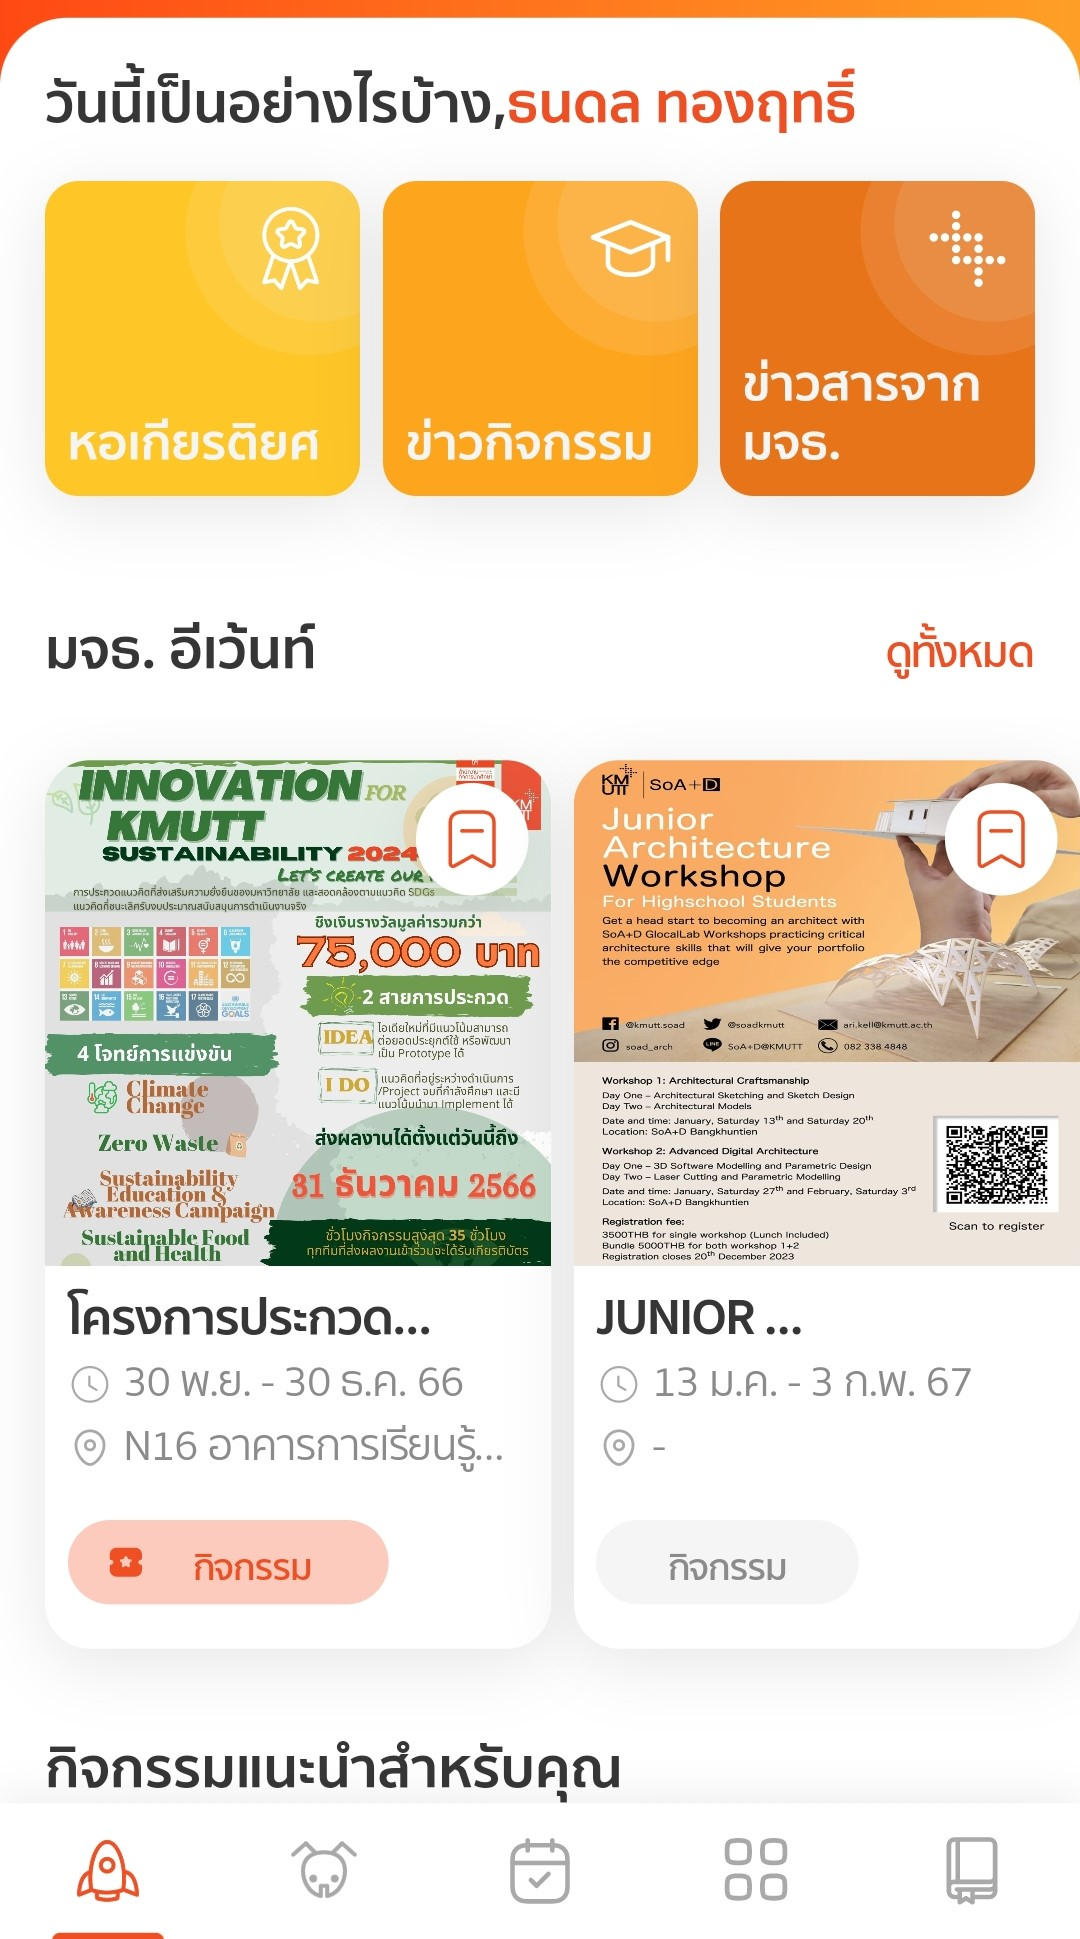
\includegraphics[width=5cm]{./modlink.jpg}}
    \caption{หน้าแนะนำกิจกรรมของ ModLink และรายละเอียด}\label{fig:modlink}
    \end{figure}

KMUTT Hatch คือ เว็บไซต์สำหรับนักศึกษาและศิษย์เก่าเพื่อประชาสัมพันธ์กิจกรรมของ Hatch ทางเว็บไซต์มีการประชามสัมพันธ์กิจกรรมต่างๆและข้อมูลที่จำเป็นต่อผู้ใช้งาน อย่างไรก็ตามเว็บไซต์นี้สามารถประชาสัมพันธ์ได้แค่กิจกรรมที่ทาง Hatch เป็นผู้จัดเท่านั้น

  \begin{figure}[!h]\centering
    \setlength{\fboxrule}{0.5mm} % can define this in the preamble
    \setlength{\fboxsep}{0.5cm}
    \fbox{
\includegraphics[width=10cm]{./hatch.png}}
    \caption{หน้าแนะนำกิจกรรมของ KMUTT Hatch}\label{fig:hatch}
    \end{figure}

\newpage

KMUTT Sinfo คือ เว็บไซต์สำหรับนักศึกษาที่ทำการรวบรวมระบบจัดการงานต่าง ๆ ของนักศึกษาไม่ว่าจะเป็นการลงทะเบียนเรียน ดูเกรด หรือประเมินกิจกรรม ซึ่งแม้ว่างานต่าง ๆ ของนักศึกษานั้นจะมีศูนย์กลางมาที่เว็บไซต์นี้ แต่ถึงกระนั้นก็เป็นเว็บที่ใช้งานไม่ค่อยสะดวก เนื่องจากต้องเข้าผ่าน pop up ซึ่งต้องอาศัยการตั้งค่าและยังใช้งานไม่ได้ในบาง platform อีกทั้งยังจำกัดเวลาที่ใช้งานเอาไว้และแม้จะเป็นศูนย์รวมประวัติการทำกิจกรรมของนักศึกษา แต่กลับไม่สามารถแนะนำได้ว่านักศึกษานั้นให้ความสนใจในกิจกรรมใด

  \begin{figure}[!h]\centering
    \setlength{\fboxrule}{0.5mm} % can define this in the preamble
    \setlength{\fboxsep}{0.5cm}
    \fbox{
\includegraphics[width=13cm]{./sinfo.png}}
    \caption{หน้า Mainpage ของ KMUTT Sinfo}\label{fig:sinfo}
    \end{figure}

\newpage

Padlet คือแอปพลิเคชันหรือเว็บไซต์ที่อยู่ในแพลตฟอร์มสำหรับ การระดมความคิด แสดงความคิดเห็น หรือแลกเปลี่ยนความรู้ร่วมกัน ผ่านกระดานดิจิทัลในรูปแบบเสมือน Post it ที่ติดบนบอร์ด ซึ่งจะแสดงผลทุกอย่างแบบ Real-time สามารถโพสต์ทั้งในรูปแบบข้อความ รูปภาพ และลิงก์ของเว็บไซต์ได้ เว็บเพจที่จะให้ผู้ใช้มาแสดงความเห็น หรือโพสต์ข้อมูลลงบนเว็บ ซึ่งจะต่างจากตรงที่ทางระบบของจะเป็นตัวกลางในการคำนวนหาจากความชื่นชอบของผู้ใช้จากกิจกรรมที่ผู้ใช้เคยได้เข้าร่วม หรือชมรมที่ผู้ใช้สนใจอยู่

  \begin{figure}[!h]\centering
    \setlength{\fboxrule}{0.5mm} % can define this in the preamble
    \setlength{\fboxsep}{0.5cm}
    \fbox{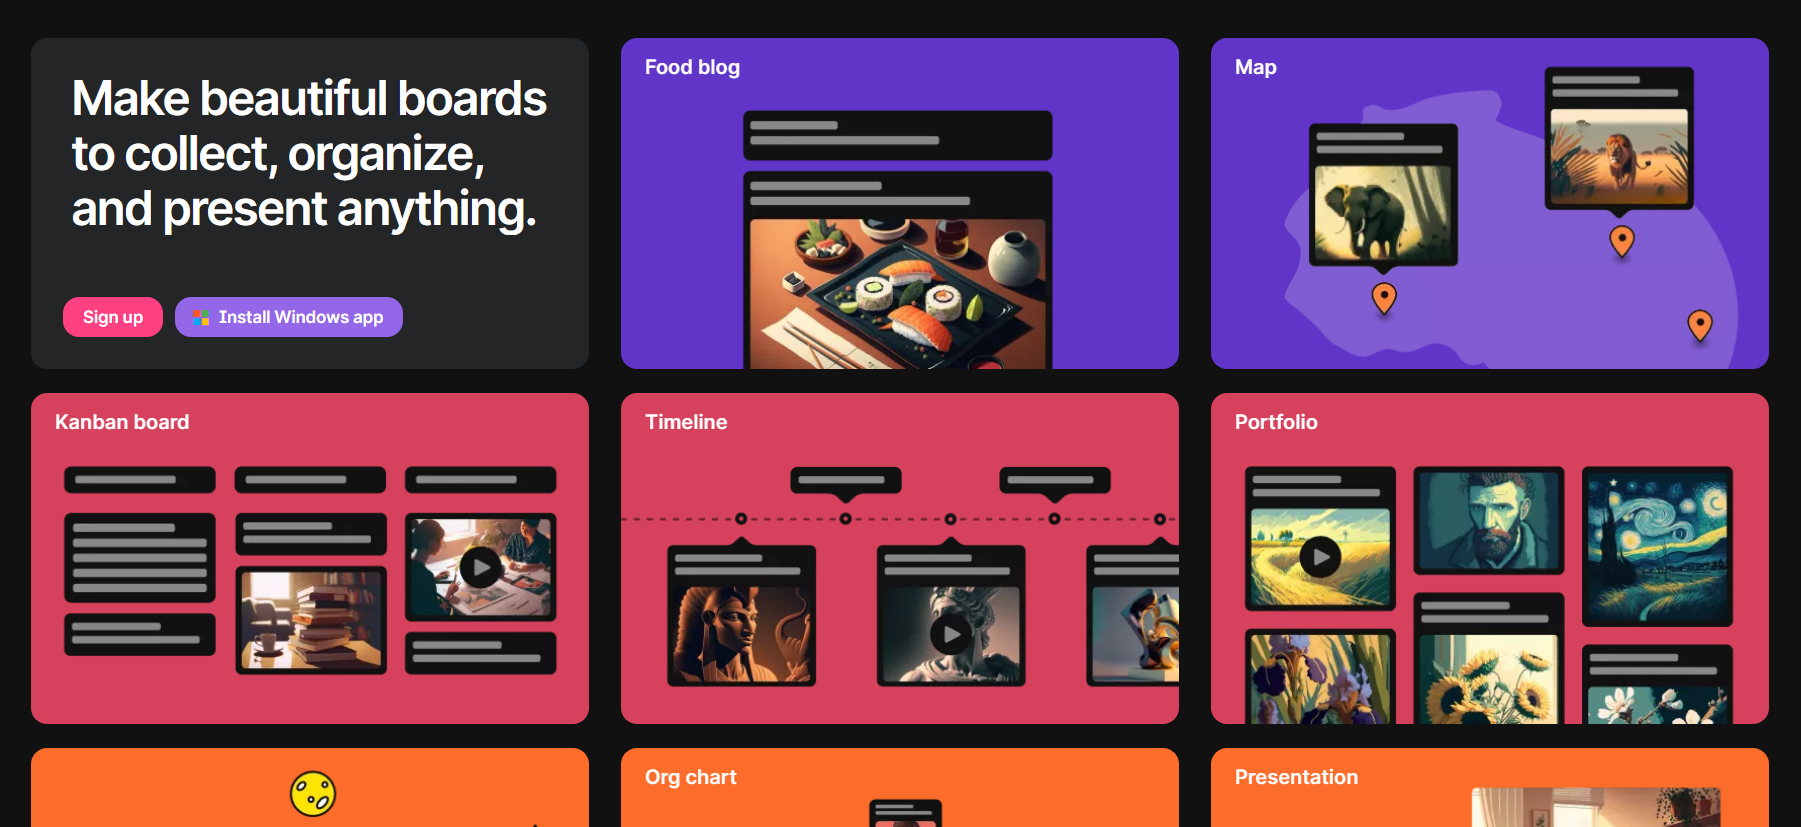
\includegraphics[width=13cm]{./padlet.png}}
    \caption{หน้า Mainpage ของ Padlet}\label{fig:padlet}
    \end{figure}

Pantip คือ พื้นที่สำหรับการแลกเปลี่ยนความคิดเห็นในหัวข้อ หรือประเด็นที่สนใจร่วมกัน สามารถสอบถาม บอกเล่าแบ่งปันประสบการณ์ในเรื่องต่าง ๆ ในหน้ากระดานสนทนาโดยสมาชิกสามารถตั้ง หรือตอบกระทู้ต่าง ๆ ที่สมาชิกสนใจและสามารถเลือกหาอ่านข้อมูลได้จากป้ายหัวข้อในเรื่องต่าง ๆ ที่ทางเว็บไซต์ ได้สร้างขึ้นไว้ ซึ่งจะต่างจากตรงที่ทางระบบของ จะเป็นตัวกลางในการคำนวนหาจากความชื่นชอบของผู้ใช้จากกิจกรรมที่ผู้ใช้เคยได้เข้าร่วม หรือชมรมที่ผู้ใช้สนใจอยู่

  \begin{figure}[!h]\centering
    \setlength{\fboxrule}{0.5mm} % can define this in the preamble
    \setlength{\fboxsep}{0.5cm}
    \fbox{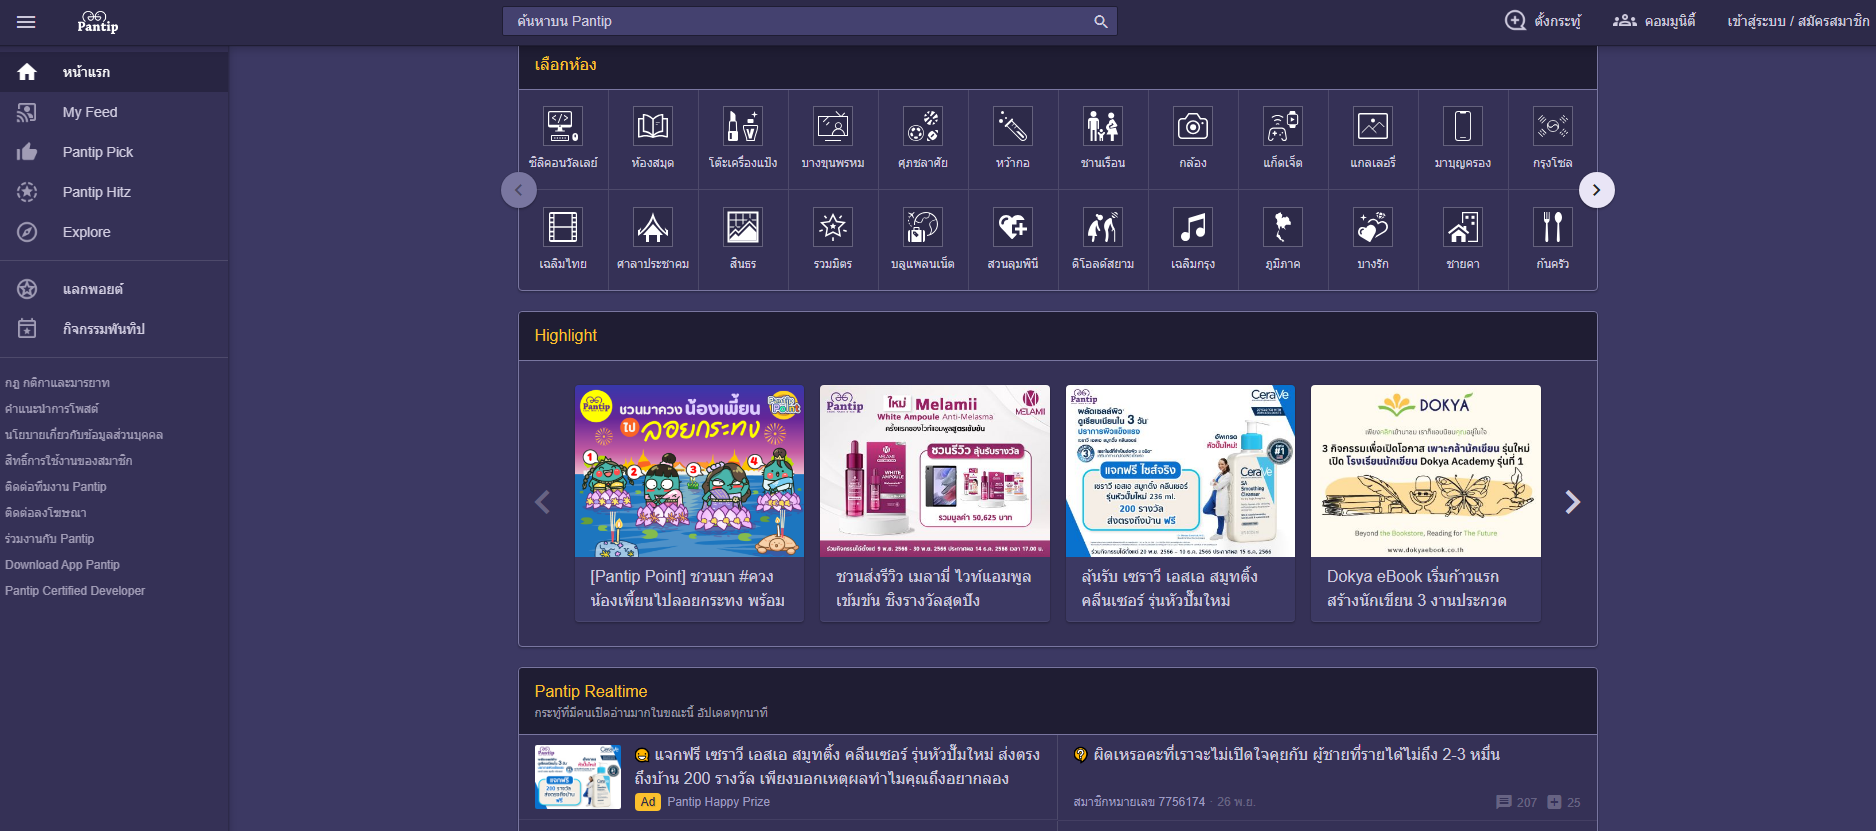
\includegraphics[width=13cm]{./pantip.png}}
    \caption{หน้าแนะนำกระทู้ของ Pantip}\label{fig:pantip}
    \end{figure}

\newpage

Facebook เป็น social media ที่ได้รับความนิยมที่สามารถใช้งาน ได้ในหลาย platform ซึ่งสามารถนำเสนอข้อมูลข่าวสารให้ผู้ใช้งานได้มากมายและเป็น social media ที่มีคนใช้งานแทบตลอดทั้งวัน ทำให้บางชมรมเลือก
ที่จะทำหน้าเพจเพื่อกระจายข่าวสารเกี่ยวกับชมรมของตัวเอง อย่างไรก็ตามด้วยปริมาณข่าวสารมากมายของ facebook ทำให้ข่าวสารของชมรมมักโดนกลบด้วย  ข่าวอื่น ๆ อยู่เสมอ ถึงแม้จะสามารถเข้าไปสู่หน้าเพจเพื่อดูความเคลื่อนไหวได้แต่ก็ไม่สามารถแนะนำตัวชมรมหรือกิจกรรมที่ชมรมจะจัดให้แก่นักศึกษาที่ไม่ติดตามเพจได้อยู่ดี

  \begin{figure}[!h]\centering
    \setlength{\fboxrule}{0.5mm} % can define this in the preamble
    \setlength{\fboxsep}{0.5cm}
    \fbox{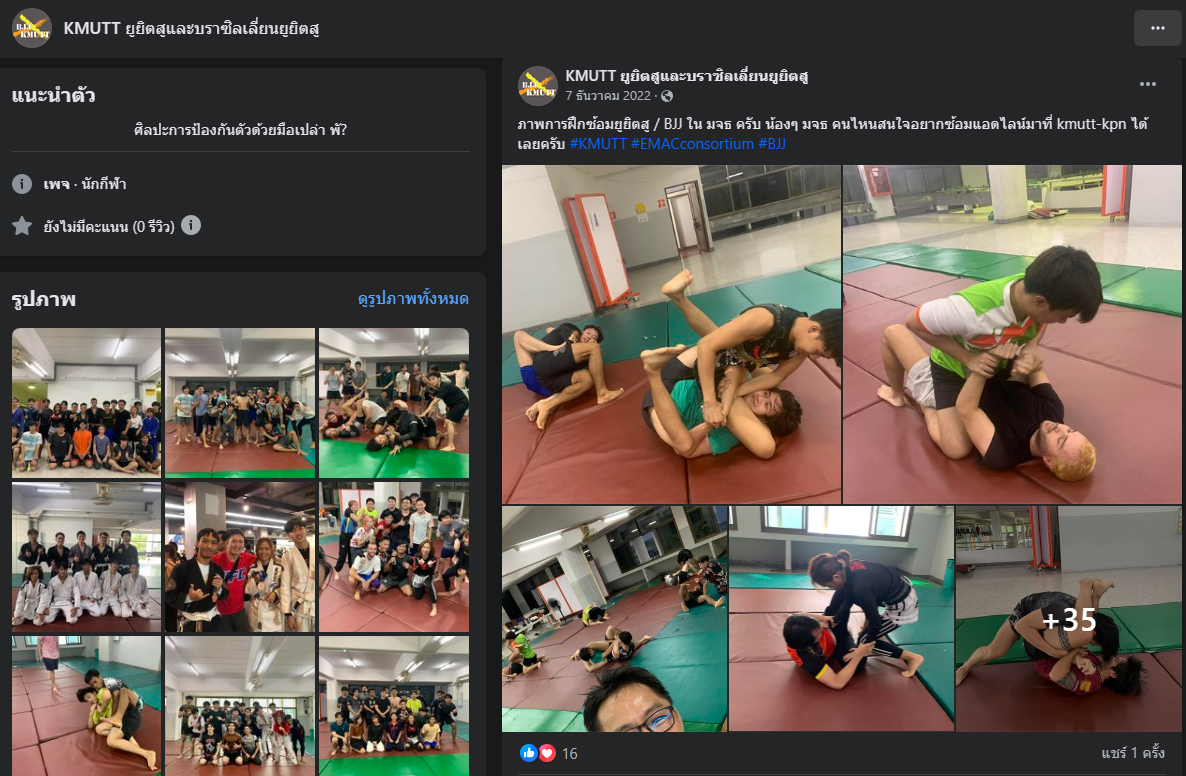
\includegraphics[width=10cm]{./facebook.png}}
    \caption{หน้า Homepage ของเพจชมรมใน Facebook}\label{fig:facebook}
    \end{figure}

\newpage

Instagram คือ แอปพลิเคชันบน smartphone และอุปกรณ์คอมพิวเตอร์ โดยแอปพลิเคชันนี้จะเน้นการแชร์รูปภาพ บน Social Network ซึ่งทำให้เพื่อน ของคุณสามารถเห็นภาพถ่ายของคุณได้และยังสามารถคอมเมนต์ภาพของคุณได้  	   ที่สำคัญ Instagram ยังสามารถแชร์ภาพของคุณไปยัง Twitter และ Facebook ได้อีกด้วย ยังสามารถกดติดตามบุคคลที่ชื่นชอบเพื่อที่จะได้เห็นโพสต์รูปภาพ วิดีโอ ของบุคคลนั้น ๆ ได้อีกด้วย และยังมีฟีเจอร์ story ที่ใช้ในการอัพรูปภาพ วิดีโอคลิปของคุณได้ด้วย

  \begin{figure}[!h]\centering
    \setlength{\fboxrule}{0.5mm} % can define this in the preamble
    \setlength{\fboxsep}{0.5cm}
    \fbox{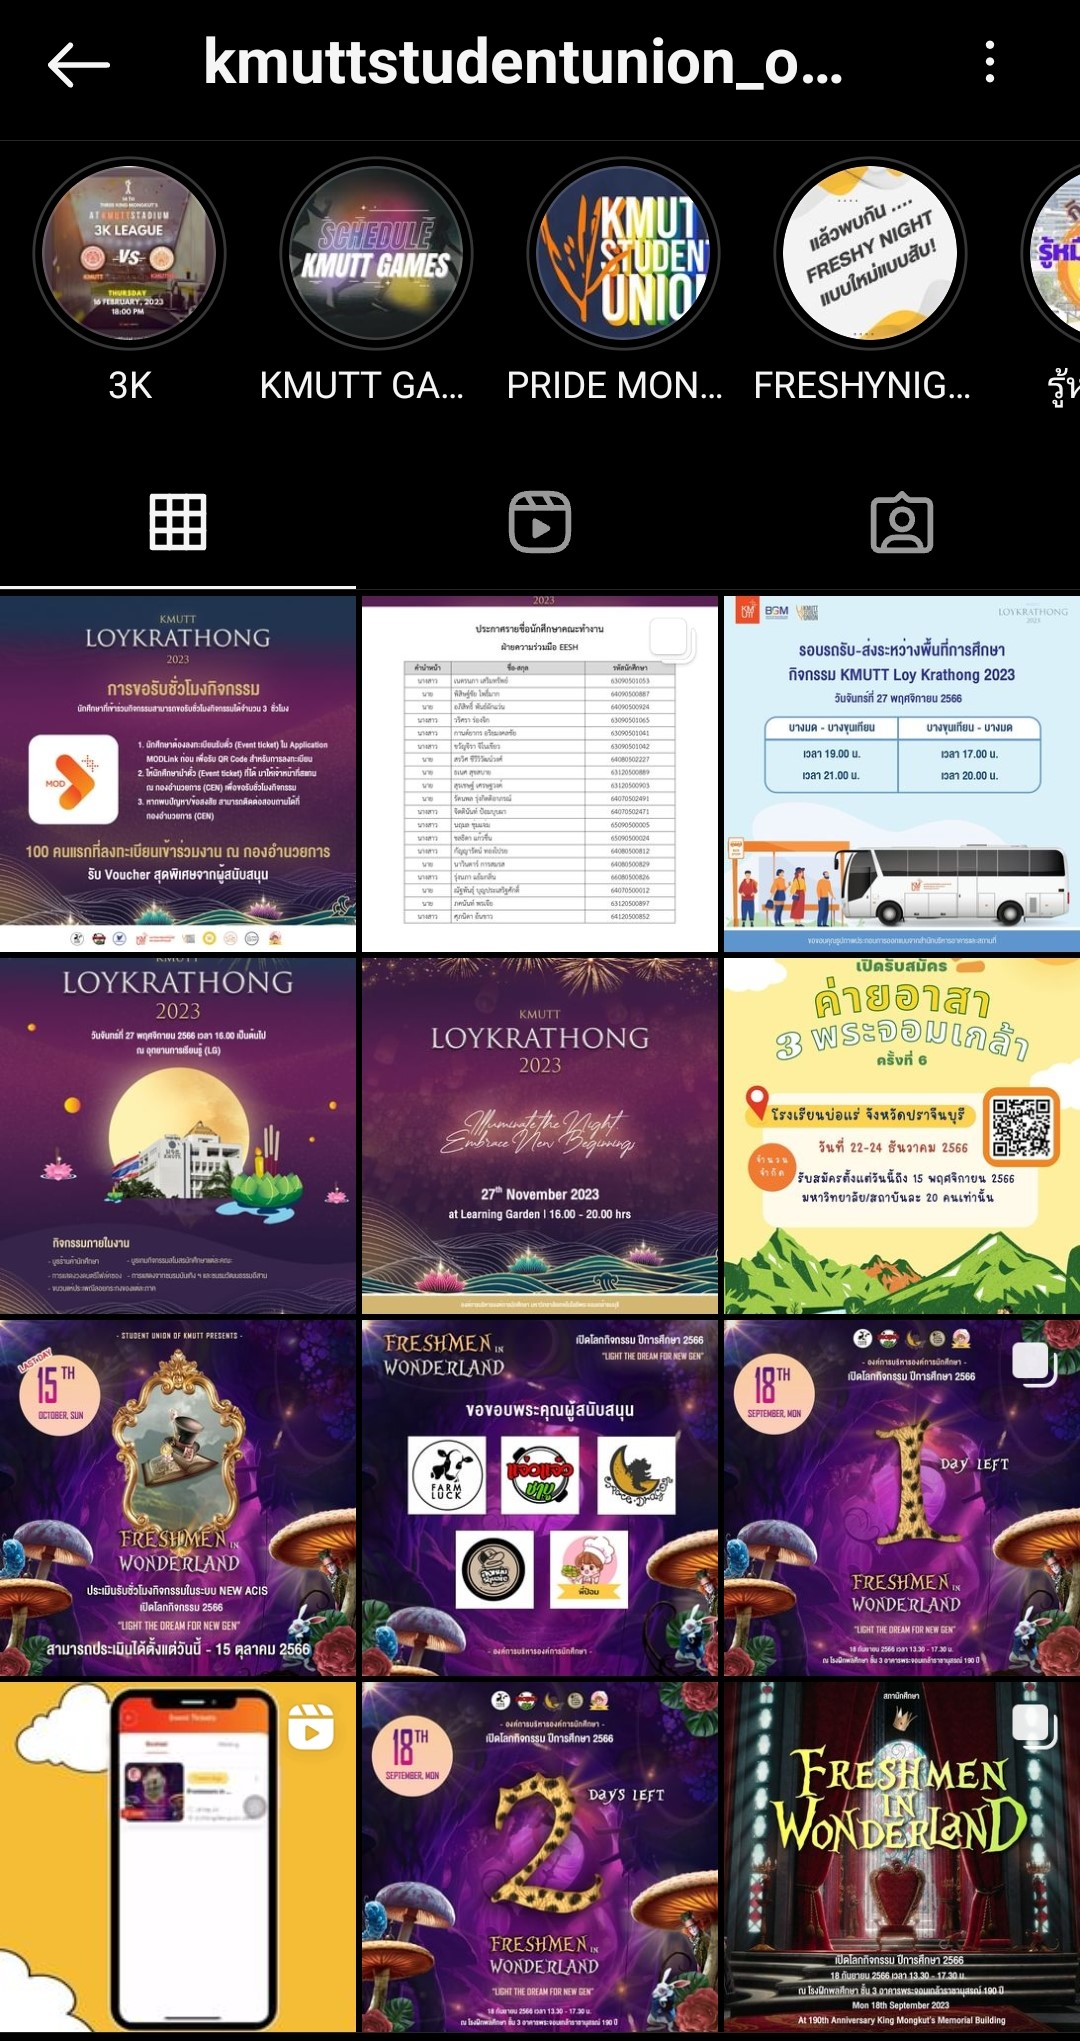
\includegraphics[width=7cm]{./ig.jpg}}
    \caption{หน้า Notifications ของ Instargram}\label{fig:ig}
    \end{figure}

\newpage

\large\textbf{ตารางความแตกต่างของ Feature}

  \begin{figure}[!h]\centering
    \setlength{\fboxrule}{0.5mm} % can define this in the preamble
    \setlength{\fboxsep}{0.5cm}
    \fbox{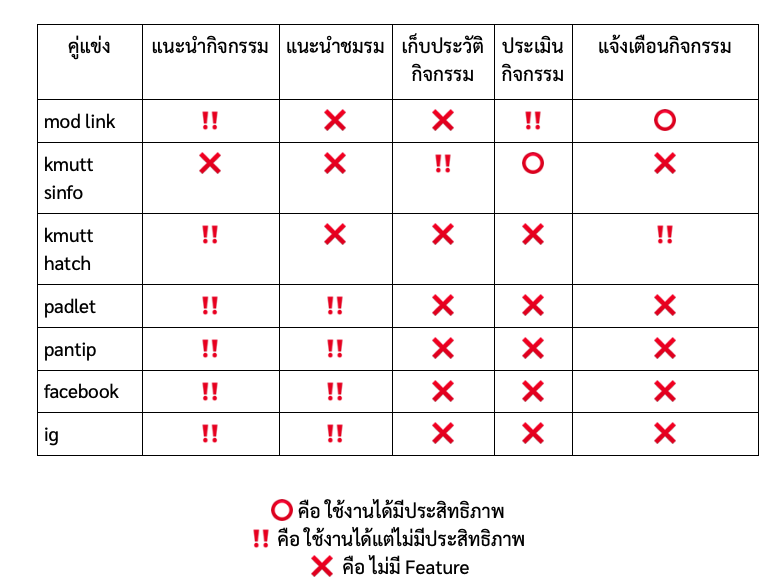
\includegraphics[width=13cm]{./DiffFeat.png}}
    \caption{ตารางความแตกต่างของ Feature}\label{fig:DiffFeat}
    \end{figure}

\newpage

\large\textbf{ระบบการแนะนำกิจกรรม} \large

  \begin{figure}[!h]\centering
    \setlength{\fboxrule}{0.5mm} % can define this in the preamble
    \setlength{\fboxsep}{0.5cm}
    \fbox{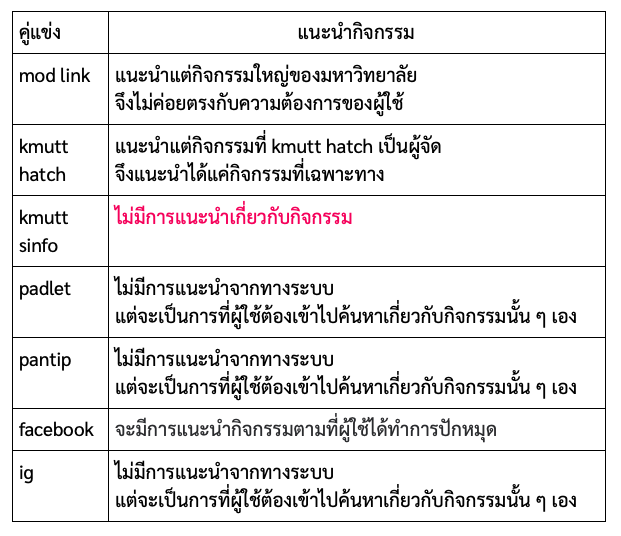
\includegraphics[width=13cm]{./Suggest.png}}
    \caption{ระบบการแนะนำกิจกรรม}\label{fig:Suggest}
    \end{figure}

\chapter{วิธีการทำงาน กระบวนการและการออกแบบ}
\section{บทนำ}
\subsection{สำรวจความต้องการของผู้ใช้เชิงคุณภาพ}
  ในการทำระบบเพื่อแจ้งเตือนข่าวสารของกิจกรรมและชมรม ทางผู้จัดทำระบุผู้ใช้งานและผู้ได้รับประโยชน์เป็น 3 กลุ่มใหญ่ๆด้วยกัน คือ ผู้เข้าร่วมกิจกรรม ผู้จัดกิจกรรม และประธานชมรม โดยแต่ล่ะกลุ่มมีความต้องการดังนี้
  ผู้เข้าร่วมกิจกรรมซึ่งเป็นผู้ใช้งานหลัก คือ นักศึกษาทั่วไปในมหาวิทยาลัย โดยมีความต้องการพื้นฐานคือการที่อยากจะทำกิจกรรมตามความสนใจ แต่ด้วยภาระการเรียนทำให้ส่วนใหญ่ไม่มีโอกาสที่จะหากิจกรรมหรือ ชมรมที่ตนเองสนใจ สิ่งที่ต้องการจึงเป็นแหล่งที่รวบรวม ข้อมูลข่าวสาร กิจกรรม และ รายละเอียดของชมรมต่างรวมถึงสิ่ง ที่ชมรมนั้นทำเอาไว้ใน ที่เดียวเพื่อที่จะหากิจกรรมและชมรมตามที่ตัวเองต้องการได้
  ผู้ได้รับประโยชน์กลุ่มแรก คือ ผู้จัดกิจกรรมที่แทนผู้จัดกิจกรรมที่เป็นเจ้าหน้าที่ของมหาวิทยาลัย โดยมีความต้องการพื้นฐานคือการประชาสัมพันธ์กิจกรรมที่จัด แต่ข่าวสารของกิจกรรมที่ถูกเผยแพร่ผ่าน platform ต่างๆ เช่น facebook หรือ instargram นั้นมีผู้ที่เห็นการประชาสัมพันธ์เพียงบางส่วนเท่านั้น ทำให้ผู้เข้าร่วมกิจกรรมมีน้อยกว่าที่คาดหวัง
  ผู้ได้รับประโยชน์กลุ่มที่ 2 คือ ประธานชมรม ที่แทนผู้ที่ดำเนินงานชมรม ซึ่งส่วนใหญ่เป็นนักศึกษาที่ใกล้จะจบการศึกษา หรือนักศึกษาชั้นปริญญาโท โดยมีความต้องการพื้นฐาน คือ การประชาสัมพันธ์ชมรมที่ตัวเองจัดการอยู่ ถึงแม้จะเป็นงานชมรมจะมี การนัดหมายกันแบบปากต่อปากอยู่แล้ว แต่การจัดการกิจกรรมชมรม ก็ไม่เป็นระบบเท่าที่ควร อีกทั้งการหาสมาชิกชมรมใหม่ หรือ การประชาสัมพันธ์กิจกรรมชมรมให้คนภายนอกชมรมนอกจากการที่ สมาชิกชมรมเป็นคนเชิญชวนก็ยังมีโอกาสที่จะมีคนเห็นการประชาสัมพันธ์ก็มีน้อย
  ซึ่งจากการสัมภาษณ์ทำให้พบว่าปัญหาใหญ่ที่เกิดขึ้นเกิดจากการที่ไม่มีแหล่งที่จะกระจายข้อมูลที่ผู้เข้าร่วมกิจกรรมต้องการในการตัดสินใจ เข้าร่วมกิจกรรม และ ชมรมได้อย่างเหมาะสม ทำให้กิจกรรม และ ชมรมไม่ได้รับความสนใจเท่าที่ควร

\subsection{Journey Map}
  จากกลุ่มผู้ใช้งานทั้งสามกลุ่มสามารถแบ่งพฤติกรรมการใช้งานได้เป็น 2 ประเภท คือ \\
  การหากิจกรรมหรือชมรม \\
  ผู้กระทำ: ผู้เข้าร่วมกิจกรรม \\
  Step 1 : ผู้เข้าร่วมกิจกรรมไปถามรายละเอียดจากผู้จัดกิจกรรมหรือประธานชมรม \\
  ปัญหา - ผู้เข้าร่วมอาจไม่รู้ว่ามีกิจกรรมหรือชมรมนี้อยู่ \\
       -  บางทีผู้เข้าร่วมกิจกรรมก็ไม่รู้จักผู้จัดกิจกรรมหรือประธานชมรม \\
  Step 2 : ผู้เข้าร่วมลงทะเบียนกิจกรรมหรือชมรม \\
  Step 3 : ผู้เข้าร่วมเข้าร่วมกิจกรรมหรือทำกิจกรรมชมรม \\
  ปัญหา - ผู้เข้าร่วมอาจไม่รู้ตำแหน่งของสถานที่จัดกิจกรรมหรือชมรม \\
  Step 4 : ผู้เข้าร่วมประเมินกิจกรรม \\
  ปัญหา - ผู้เข้าร่วมไม่รู้ว่าแบบประเมินกิจกรรมสามารถประเมินได้แล้ว \\

\subsection{Stakeholder}
  ผู้ที่คาดว่าจะได้รับประโยชน์จากการใช้งานแอปพลิเคชันของผู้จัดทำสร้างขึ้นนั้นแบ่งเป็น 2 กลุ่ม คือ ผู้เข้าร่วมกิจกรรม และ ฝั่งผู้จัดกิจกรรมที่หมายถึงผู้จัดกิจกรรมและประธานชมรม \\
  ฝั่งผู้เข้าร่วมกิจกรรม คือ นักศึกษาชั้นปีที่ 1 เนื่องจากเป็นกลุ่มที่ยังมีข้อมูลเกี่ยวกับสิ่งต่าง ๆ ในมหาวิทยาลัยอยู่น้อยทำให้ยากที่จะหาแหล่งข้อมูลของกิจกรรมหรือชมรมที่สนใจ \\
  ฝั่งผู้จัดกิจกรรม คือ นักศึกษาชั้นปีที่ 4 ที่เป็นประธานชมรมและผู้จัดกิจกรรมที่เป็นเจ้าหน้าที่ของมหาวิทยาลัย เนื่องจากเป็นผู้ได้รับผลกระทบจากการประชาสัมพันธ์กิจกรรมและชมรมที่ไม่มีประสิทธิภาพเท่าที่ควร \\

\section{Requirement list}
  รายการข้อกำหนดหรือความต้องการที่จำเป็นต้องมีในโครงการหรือผลิตภัณฑ์ที่กำลังถูกพัฒนา ข้อกำหนดเหล่านี้เป็นข้อมูลที่ถูกรวบรวมมาจากผู้ใช้, ลูกค้า, หรือผู้เกี่ยวข้องอื่น ๆ ซึ่งมีไว้เพื่อกำหนดขอบเขตและคุณลักษณะของผลิตภัณฑ์หรือโครงการ โดยในส่วนนี้ หลังจากที่ได้ทำการ สำรวจความต้องการจาก Early Adopter แล้วทำให้เราได้ความต้องการมา ดังนี้ \\

\begin{enumerate}
  \item ข้อมูลของกิจกรรมและชมรมที่ชัดเจน
  \item ระบบการค้นหากิจกรรมและชมรม
  \item การแนะนำชมรมและกิจกรรมที่ที่น่าสนใจ
  \item การแจ้งเตือนการประเมินกิจกรรม
\end{enumerate}

\section{Feature list}
  จากการวิเคราะห์ Requirement ทั้งหมด เราได้ทำการวิเคราะห์ feature มาเพื่อตอบโจทย์ความต้องการของผู้ใช้ดังนี้
\begin{enumerate}
  \item Login: ลงชื่อเพื่อเข้าใช้งานแอพพลิเคชัน
  \item Registration: สมัครบัญชีของแอพพลิเคชันด้วยอีเมลมหาวิทยาลัย
  \item Logout: ออกจากระบบ
  \item Search: ค้นหากิจกรรมหรือชมรมที่สนใจ
  \item Select: เลือกอ่านรายละเอียดกิจกรรมหรือชมรมที่สนใจ
  \item Join: 
  \begin{itemize}
    \item ลงชื่อเข้าร่วมกิจกรรมที่สนใจ
    \item ลงชื่อเป็นสมาชิกของชมรมที่สนใจ
  \end{itemize}
  \item Resignation: ถอนชื่อจากการเป็นสมาชิกชมรม
  \item Notification: 
  \begin{itemize}
    \item แจ้งเตือนกิจกรรมที่เกี่ยวข้องกับชมรมหรือความสนใจของนักศึกษา
    \item แจ้งเตือนการประเมินกิจกรรม
  \end{itemize}
  \item Event evaluation: ประเมินกิจกรรม
  \item Recommendation: แนะนำกิจกรรมและชมรม ตามความสนใจของผู้ใช้โดยอ้างอิงจาก tag ของกิจกรรม
\end{enumerate}

\newpage

\section{Architecture diagram}

  \begin{figure}[!h]\centering
    \setlength{\fboxrule}{0.5mm} % can define this in the preamble
    \setlength{\fboxsep}{0.5cm}
    \fbox{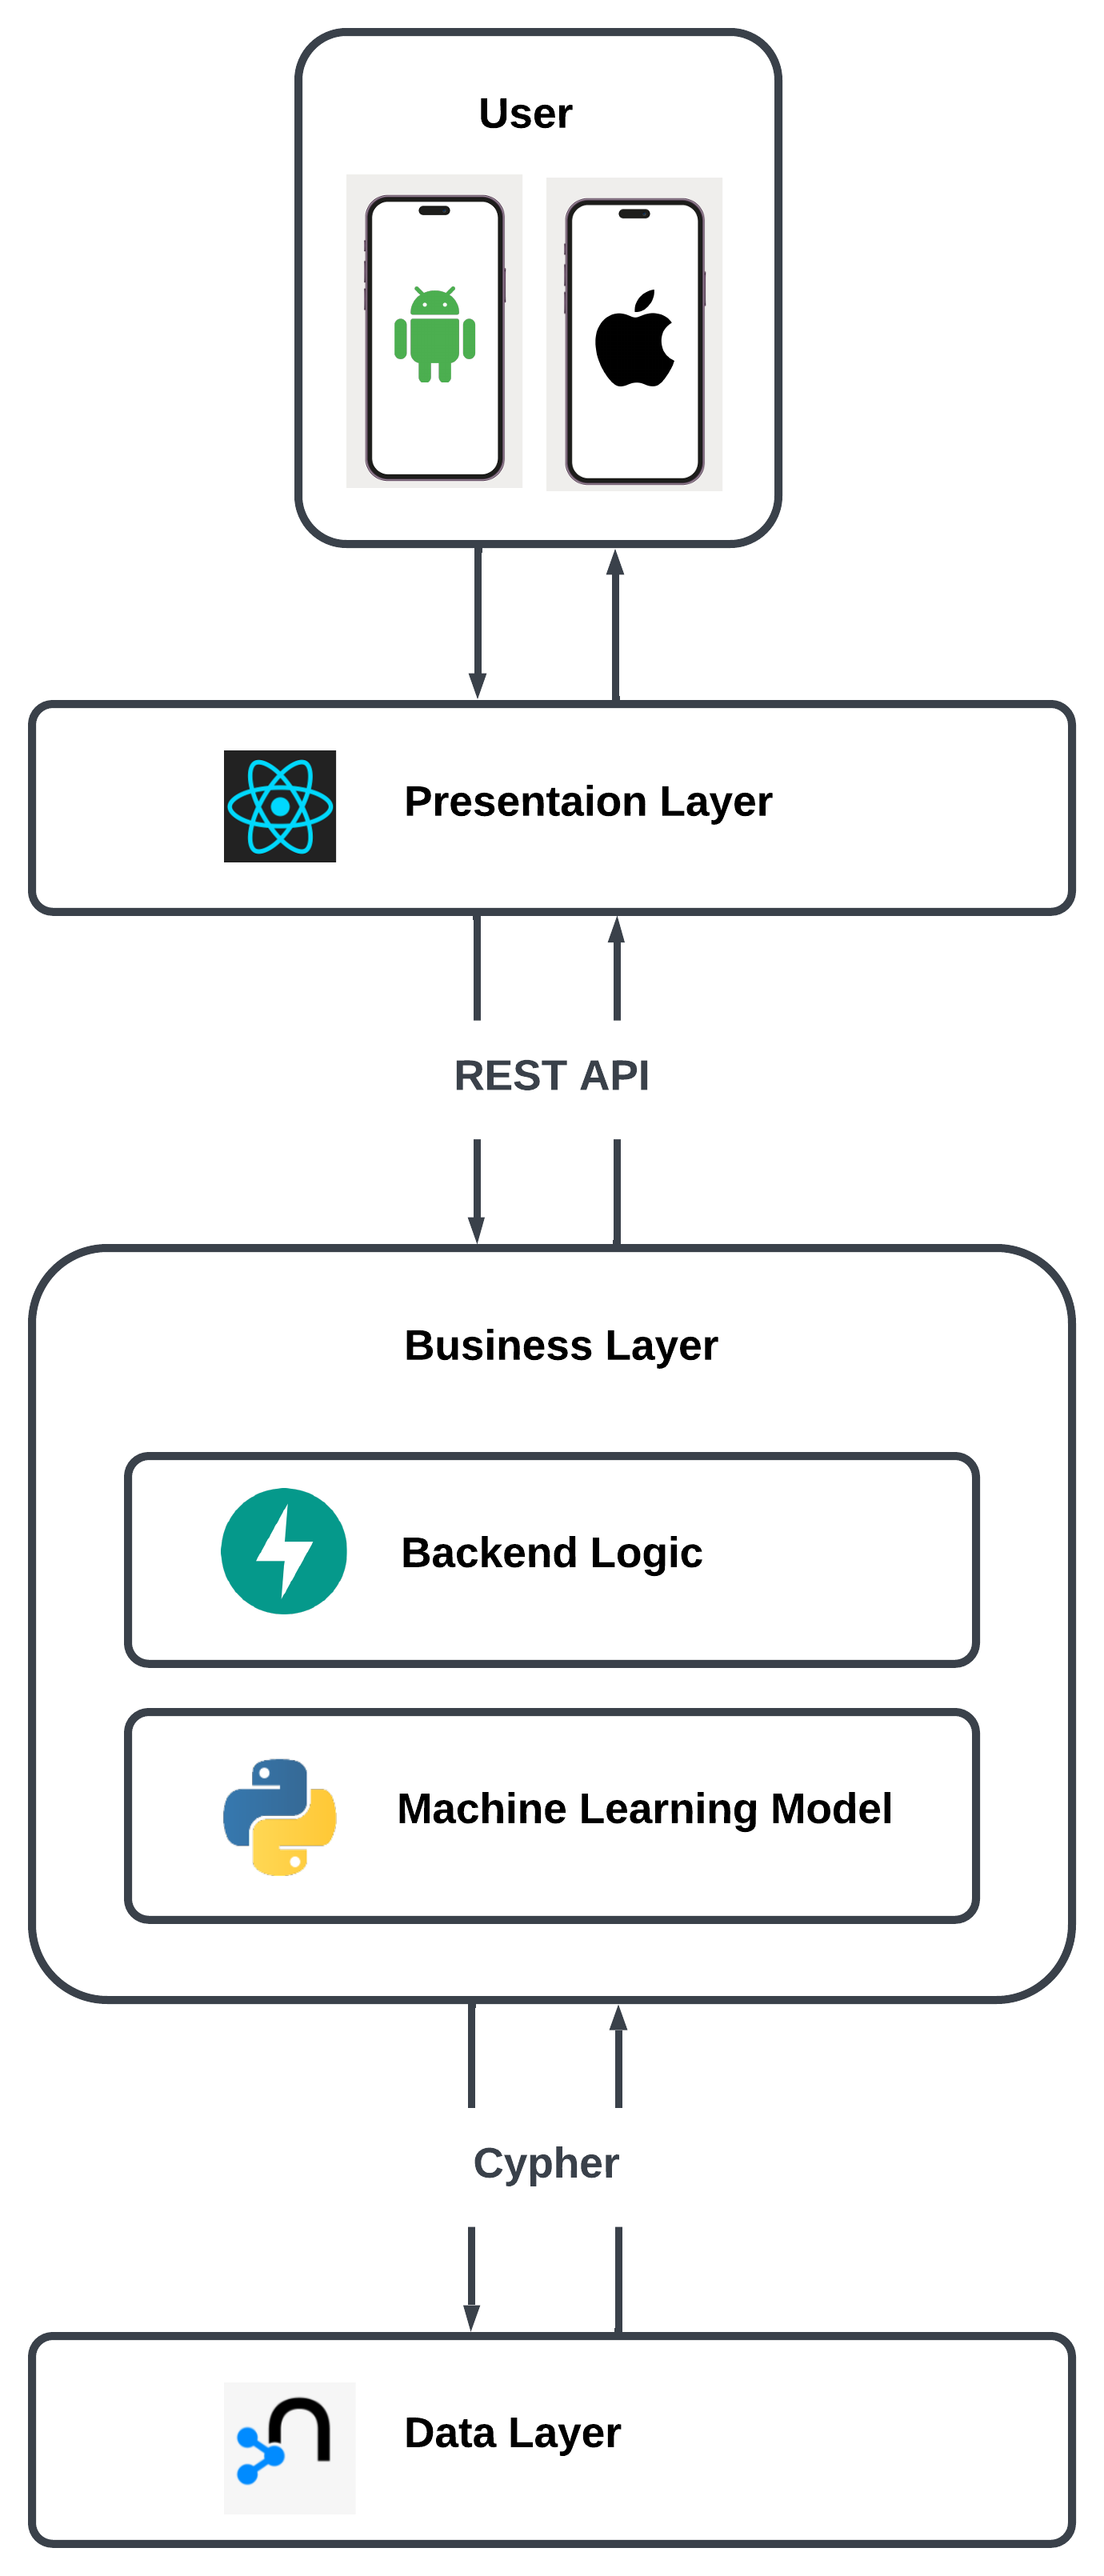
\includegraphics[width=7cm]{./ArchDia.png}}
    \caption{Architecture diagram}\label{fig:ArchDia}
    \end{figure}

\newpage

System Flow
\begin{enumerate}
  \item User ใช้งาน React Native Application
  \item React Native ส่ง HTTP request ตามรูปแบบของ Rest API ที่กำหนดไว้ ไปยัง FastAPI backend เพื่อเรียกใช้งานฟังก์ชันต่าง ๆ เช่น ค้นหากิจกรรมหรือดูข้อมูลเกี่ยวกับชมรม เป็นต้น
  \item FastAPI ประมวลผล request และส่ง request เพิ่มเติมด้วย Cypher ไปยัง Neo4j database เพื่อขอข้อมูล หรือเปลี่ยนแปลงข้อมูล
    สำหรับการแนะนำและการประมวลผลข้อมูลกิจกรรมหรือชมรม FastAPI จะติดต่อกับ Machine Learning Model เพิ่มเติม
  \item Neo4j ประมวลผลข้อมูลตาม request ของ FastAPI
  \item FastAPI ส่ง HTTP response กลับไปยัง React Native และ React Native ปรับเปลี่ยน User Interface ตาม response ที่ได้รับ
\end{enumerate}

\section{Use case diagram and use case narratives}

  \begin{figure}[!h]\centering
    \setlength{\fboxrule}{0.5mm} % can define this in the preamble
    \setlength{\fboxsep}{0.5cm}
    \fbox{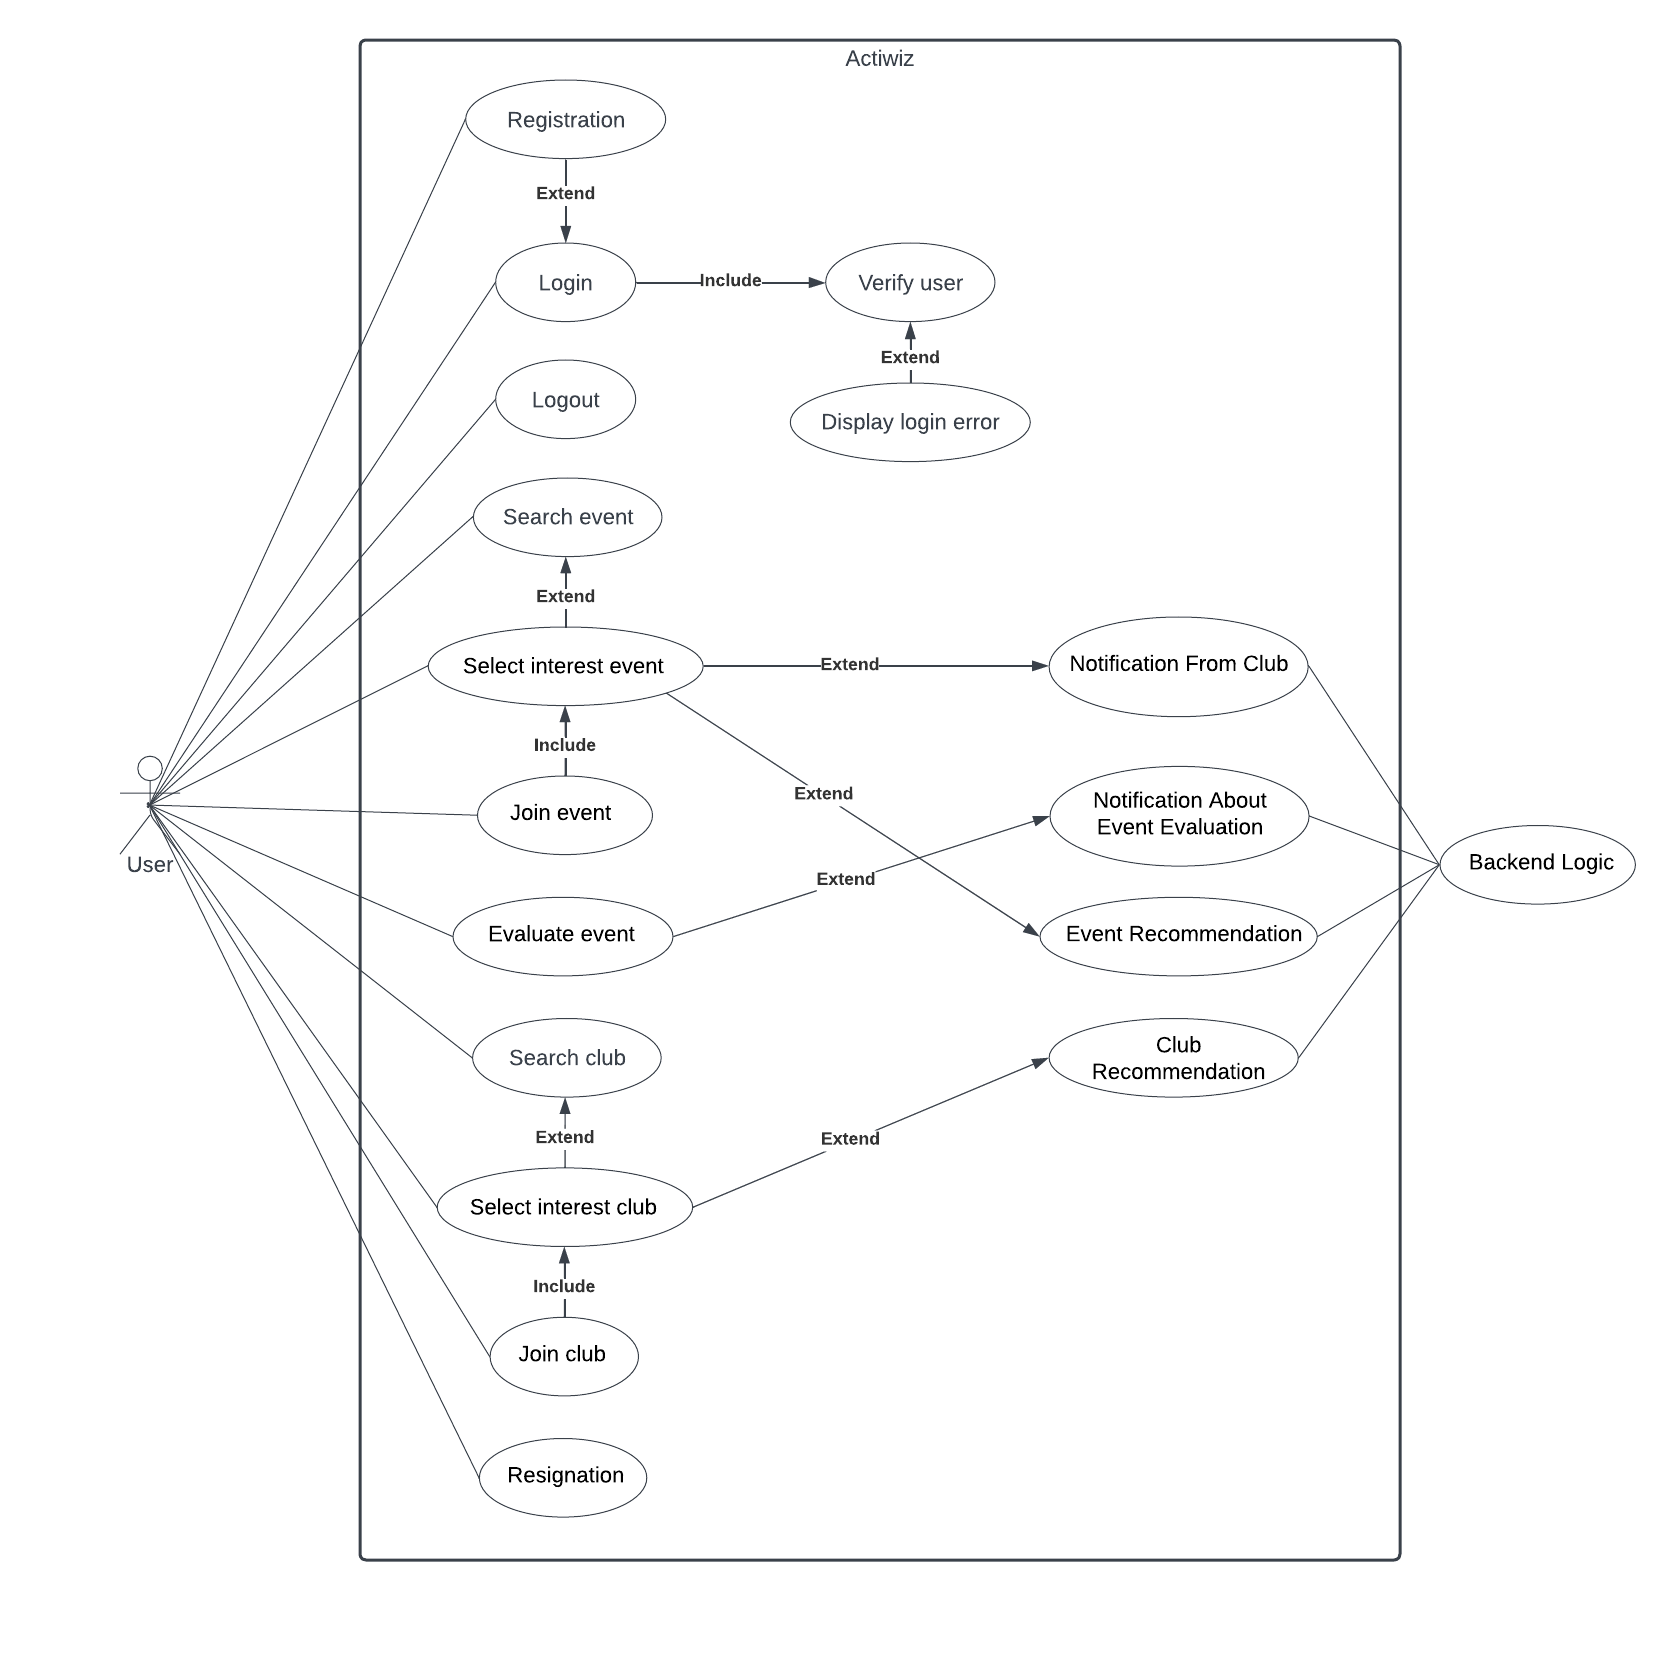
\includegraphics[width=7cm]{./usedcase.png}}
    \caption{Use case diagram and use case narratives}\label{fig:usecasediagram}
  \end{figure}

\newpage

\textbf{Use case narratives} \\
use case diagram นี้เป็นการแสดงการทำงานของระบบและการใช้งานจากผู้ใช้งาน ใช้ case diagram ในการแสดงภาพรวมของระบบและลำดับการทำงานของฟังก์ชันใช้งานในระบบ โดยมีผู้กระทำหลักคือ User และผู้กระทำรองคือ Backed Logic


Registration scenario
\\
\begin{table}[!h]\centering 
  \begin{tabular}{|
  >{\columncolor[HTML]{FFFFFF}}c |c|}
  \hline
  \cellcolor[HTML]{6D9EEB}Actor         & \cellcolor[HTML]{6D9EEB}User                   \\ \hline
  {\color[HTML]{0A0A23} Goal}           & \cellcolor[HTML]{FFFFFF}ลงทะเบียนสร้าง account \\ \hline
  {\color[HTML]{0A0A23} Pre-conditions} & -                                              \\ \hline
  {\color[HTML]{0A0A23} Main success scenario} &
    \begin{tabular}[c]{@{}c@{}}1.User ทำการกดเข้าหน้าลงทะเบียน\\ 2.User กรอกแบบฟอร์ม\\ 3.User กดยืนยันการสร้าง account\end{tabular} \\ \hline
  \end{tabular}
  \caption{\centering Registration scenario}\label{fig:Registration scenario}
\end{table}

Login scenario

\begin{table}[!h]\centering 
  \begin{tabular}{|l|l|}
  \hline
  \rowcolor[HTML]{6D9EEB} 
  \multicolumn{1}{|c|}{\cellcolor[HTML]{6D9EEB}Actor} & \multicolumn{1}{c|}{\cellcolor[HTML]{6D9EEB}User} \\ \hline
  \rowcolor[HTML]{FFFFFF} 
  {\color[HTML]{0A0A23} Actor}                        & \cellcolor[HTML]{FFFFFF}User                      \\ \hline
  \cellcolor[HTML]{FFFFFF}{\color[HTML]{0A0A23} Goal} & เข้าสู่ระบบและใช้งานฟังก์ชันต่างได้               \\ \hline
  \cellcolor[HTML]{FFFFFF}{\color[HTML]{0A0A23} Pre-conditions} &
    \begin{tabular}[c]{@{}l@{}}-User จำเป็นต้องลงทะเบียน account ก่อน\\ -User จำเป็นต้องยืนยัน account ก่อน\end{tabular} \\ \hline
  Main success scenario &
    \begin{tabular}[c]{@{}l@{}}1.User กรอกอีเมลและรหัสผ่าน\\ 2.User เข้าสู่ homepage ของแอปพลิเคชัน\\ 3.ระบบแสดงฟังก์ชันที่ใช้งานได้ทั้งหมด\\ 4.Userใช้งานฟังก์ชันต่างๆในแอปพลิเคชัน\end{tabular} \\ \hline
  \end{tabular}
  \caption{\centering Login scenario}\label{fig:Login scenario}
\end{table}

Logout cenario

\begin{table}[!h]\centering 
  \begin{tabular}{|c|c|}
  \hline
  \rowcolor[HTML]{6D9EEB} 
  Actor                                               & User                         \\ \hline
  \rowcolor[HTML]{FFFFFF} 
  {\color[HTML]{0A0A23} Actor}                        & \cellcolor[HTML]{FFFFFF}User \\ \hline
  \cellcolor[HTML]{FFFFFF}{\color[HTML]{0A0A23} Goal} & ออกจากระบบ                   \\ \hline
  \cellcolor[HTML]{FFFFFF}{\color[HTML]{0A0A23} Pre-conditions} & -User ต้องเข้าสู่ระบบก่อน \\ \hline
  Main success scenario                               & User ทำการกดออกจากระบบ     \\ \hline
  \end{tabular}
  \caption{\centering Logout scenario}\label{fig:Logout scenario}
\end{table}

\newpage

Search event scenario

\begin{table}[!h]\centering 
  \begin{tabular}{|c|c|}
  \hline
  \rowcolor[HTML]{6D9EEB} 
  Actor                                               & User                         \\ \hline
  \rowcolor[HTML]{FFFFFF} 
  {\color[HTML]{0A0A23} Actor}                        & \cellcolor[HTML]{FFFFFF}User \\ \hline
  \cellcolor[HTML]{FFFFFF}{\color[HTML]{0A0A23} Goal} & ค้นหากิจกรรม                 \\ \hline
  \cellcolor[HTML]{FFFFFF}{\color[HTML]{0A0A23} Pre-conditions} & - User ต้องเข้าสู่ระบบก่อน                                                                        \\ \hline
  Main success scenario                                         & \begin{tabular}[c]{@{}c@{}}1.User ค้นหากิจกรรมที่ต้องการ\\ 2.ระบบแสดงกิจกรรมที่ค้นหา\end{tabular} \\ \hline
  \end{tabular}
  \caption{\centering Search event scenario}\label{fig:Search event scenario}
\end{table}

Select event scenario

\begin{table}[!h]\centering 
  \begin{tabular}{|c|c|}
  \hline
  \rowcolor[HTML]{6D9EEB} 
  Actor                                                         & User                                          \\ \hline
  \rowcolor[HTML]{FFFFFF} 
  {\color[HTML]{0A0A23} Goal}                                   & \cellcolor[HTML]{FFFFFF}อ่านรายละเอียดกิจกรรม \\ \hline
  \cellcolor[HTML]{FFFFFF}{\color[HTML]{0A0A23} Pre-conditions} & - User ต้องเข้าสู่ระบบก่อน                    \\ \hline
  \cellcolor[HTML]{FFFFFF}{\color[HTML]{0A0A23} Main success scenario} &
    \begin{tabular}[c]{@{}c@{}}1.User กดไปที่กิจกรรมที่สนใจ\\ 2.ระบบแสดงรายละเอียดกิจกรรมที่ค้นหา\end{tabular} \\ \hline
  Main success scenario &
    \begin{tabular}[c]{@{}c@{}}1.User ค้นหากิจกรรมที่ต้องการ\\ 2.ระบบแสดงกิจกรรมที่ค้นหา\end{tabular} \\ \hline
  \end{tabular}
  \caption{\centering Select event scenario}\label{fig:Select event scenario}
\end{table}

Join event scenario

\begin{table}[!h]\centering 
  \begin{tabular}{|c|c|}
  \hline
  \rowcolor[HTML]{6D9EEB} 
  Actor                       & User                                    \\ \hline
  \rowcolor[HTML]{FFFFFF} 
  {\color[HTML]{0A0A23} Goal} & \cellcolor[HTML]{FFFFFF}เข้าร่วมกิจกรรม \\ \hline
  \cellcolor[HTML]{FFFFFF}{\color[HTML]{0A0A23} Pre-conditions} &
    \begin{tabular}[c]{@{}c@{}}- User ต้องเข้าสู่ระบบก่อน\\ - User ต้องเข้าสู่หน้าอ่านรายละเอียดกิจกรรมก่อน\end{tabular} \\ \hline
  \cellcolor[HTML]{FFFFFF}{\color[HTML]{0A0A23} Main success scenario} &
    \begin{tabular}[c]{@{}c@{}}1.User กดเข้าร่วมกิจกรรม\\ 2.ระบบพาไปยังหน้ากรอกแบบฟอร์มของกิจกรรม\end{tabular} \\ \hline
  Main success scenario &
    \begin{tabular}[c]{@{}c@{}}1.User ค้นหากิจกรรมที่ต้องการ\\ 2.ระบบแสดงกิจกรรมที่ค้นหา\end{tabular} \\ \hline
  \end{tabular}
  \caption{\centering Join event scenario}\label{fig:Join event scenario}
\end{table}

\newpage

Evaluate event scenario

\begin{table}[!h]\centering 
  \begin{tabular}{|c|c|}
  \hline
  \rowcolor[HTML]{6D9EEB} 
  Actor                                                         & User                                   \\ \hline
  \rowcolor[HTML]{FFFFFF} 
  {\color[HTML]{0A0A23} Goal}                                   & \cellcolor[HTML]{FFFFFF}ประเมินกิจกรรม \\ \hline
  \cellcolor[HTML]{FFFFFF}{\color[HTML]{0A0A23} Pre-conditions} & - User ต้องเข้าสู่ระบบก่อน             \\ \hline
  \cellcolor[HTML]{FFFFFF}{\color[HTML]{0A0A23} Main success scenario} &
    \begin{tabular}[c]{@{}c@{}}1.User ได้รับแจ้งเตือนการประเมินกิจกรรม\\ 2.User กดเข้าประเมินกิจกรรม\\ 3.ระบบพาไปหน้าประเมินกิจกรรม\end{tabular} \\ \hline
  Main success scenario &
    \begin{tabular}[c]{@{}c@{}}1.User ได้รับแจ้งเตือนการประเมินกิจกรรม\\ 2.User กดเข้าประเมินกิจกรรม\\ 3.ระบบพาไปหน้าประเมินกิจกรรม\end{tabular} \\ \hline
  \end{tabular}
  \caption{\centering Evaluate event scenario}\label{fig:Evaluate event scenario}
\end{table}

Search club scenario

\begin{table}[!h]\centering 
  \begin{tabular}{|c|c|}
  \hline
  \rowcolor[HTML]{6D9EEB} 
  Actor                                                         & User                              \\ \hline
  \rowcolor[HTML]{FFFFFF} 
  {\color[HTML]{0A0A23} Goal}                                   & \cellcolor[HTML]{FFFFFF}ค้นหาชมรม \\ \hline
  \cellcolor[HTML]{FFFFFF}{\color[HTML]{0A0A23} Pre-conditions} & - User ต้องเข้าสู่ระบบก่อน        \\ \hline
  \cellcolor[HTML]{FFFFFF}{\color[HTML]{0A0A23} Main success scenario} &
    \begin{tabular}[c]{@{}c@{}}1.User ค้นหาชมรมที่ต้องการ\\ 2.ระบบแสดงชมรมที่ค้นหา\end{tabular} \\ \hline
  Main success scenario &
    \begin{tabular}[c]{@{}c@{}}1.User ได้รับแจ้งเตือนการประเมินกิจกรรม\\ 2.User กดเข้าประเมินกิจกรรม\\ 3.ระบบพาไปหน้าประเมินกิจกรรม\end{tabular} \\ \hline
  \end{tabular}
  \caption{\centering Search club scenario}\label{fig:Search club scenario}
\end{table}

Select club scenario

\begin{table}[!h]\centering 
  \begin{tabular}{|c|c|}
  \hline
  \rowcolor[HTML]{6D9EEB} 
  Actor                                                         & User                                       \\ \hline
  \rowcolor[HTML]{FFFFFF} 
  {\color[HTML]{0A0A23} Goal}                                   & \cellcolor[HTML]{FFFFFF}อ่านรายละเอียดชมรม \\ \hline
  \cellcolor[HTML]{FFFFFF}{\color[HTML]{0A0A23} Pre-conditions} & - User ต้องเข้าสู่ระบบก่อน                 \\ \hline
  \cellcolor[HTML]{FFFFFF}{\color[HTML]{0A0A23} Main success scenario} &
    \begin{tabular}[c]{@{}c@{}}1.User กดไปที่ชมรมที่สนใจ\\ 2.ระบบแสดงรายละเอียดชมรมที่ค้นหา\end{tabular} \\ \hline
  Main success scenario &
    \begin{tabular}[c]{@{}c@{}}1.User ได้รับแจ้งเตือนการประเมินกิจกรรม\\ 2.User กดเข้าประเมินกิจกรรม\\ 3.ระบบพาไปหน้าประเมินกิจกรรม\end{tabular} \\ \hline
  \end{tabular}
  \caption{\centering Select club scenario}\label{fig:Select club scenario}
\end{table}

\newpage

Join club scenario

\begin{table}[!h]\centering 
  \begin{tabular}{|c|c|}
  \hline
  \rowcolor[HTML]{6D9EEB} 
  Actor                                                                & User                                 \\ \hline
  \rowcolor[HTML]{FFFFFF} 
  {\color[HTML]{0A0A23} Goal}                                          & \cellcolor[HTML]{FFFFFF}เข้าร่วมชมรม \\ \hline
  \cellcolor[HTML]{FFFFFF}{\color[HTML]{0A0A23} Pre-conditions} &
    \begin{tabular}[c]{@{}c@{}}- User ต้องเข้าสู่ระบบก่อน\\ - User ต้องเข้าสู่หน้าอ่านรายละเอียดชมรมก่อน\end{tabular} \\ \hline
  \cellcolor[HTML]{FFFFFF}{\color[HTML]{0A0A23} Main success scenario} & 1.User กดเข้าร่วมชมรม                \\ \hline
  Main success scenario &
    \begin{tabular}[c]{@{}c@{}}1.User ได้รับแจ้งเตือนการประเมินกิจกรรม\\ 2.User กดเข้าประเมินกิจกรรม\\ 3.ระบบพาไปหน้าประเมินกิจกรรม\end{tabular} \\ \hline
  \end{tabular}
  \caption{\centering Join club scenario}\label{fig:Join club scenario}
\end{table}

Resignation scenario

\begin{table}[!h]\centering 
  \begin{tabular}{|c|c|}
  \hline
  \rowcolor[HTML]{6D9EEB} 
  Actor                                                                & User                                 \\ \hline
  \rowcolor[HTML]{FFFFFF} 
  {\color[HTML]{0A0A23} Goal}                                          & \cellcolor[HTML]{FFFFFF}เข้าร่วมชมรม \\ \hline
  \cellcolor[HTML]{FFFFFF}{\color[HTML]{0A0A23} Pre-conditions} &
    \begin{tabular}[c]{@{}c@{}}- User ต้องเข้าสู่ระบบก่อน\\ - User ต้องเข้าสู่หน้าอ่านรายละเอียดชมรมก่อน\end{tabular} \\ \hline
  \cellcolor[HTML]{FFFFFF}{\color[HTML]{0A0A23} Main success scenario} & 1.User กดเข้าร่วมชมรม                \\ \hline
  Main success scenario &
    \begin{tabular}[c]{@{}c@{}}1.User ได้รับแจ้งเตือนการประเมินกิจกรรม\\ 2.User กดเข้าประเมินกิจกรรม\\ 3.ระบบพาไปหน้าประเมินกิจกรรม\end{tabular} \\ \hline
  \end{tabular}
  \caption{\centering Resignation scenario}\label{fig:Resignation scenario}
\end{table}

\newpage

\section{Sequence diagram}
\subsection{Login}

  \begin{figure}[!h]\centering
    \setlength{\fboxrule}{0.5mm} % can define this in the preamble
    \setlength{\fboxsep}{0.5cm}
    \fbox{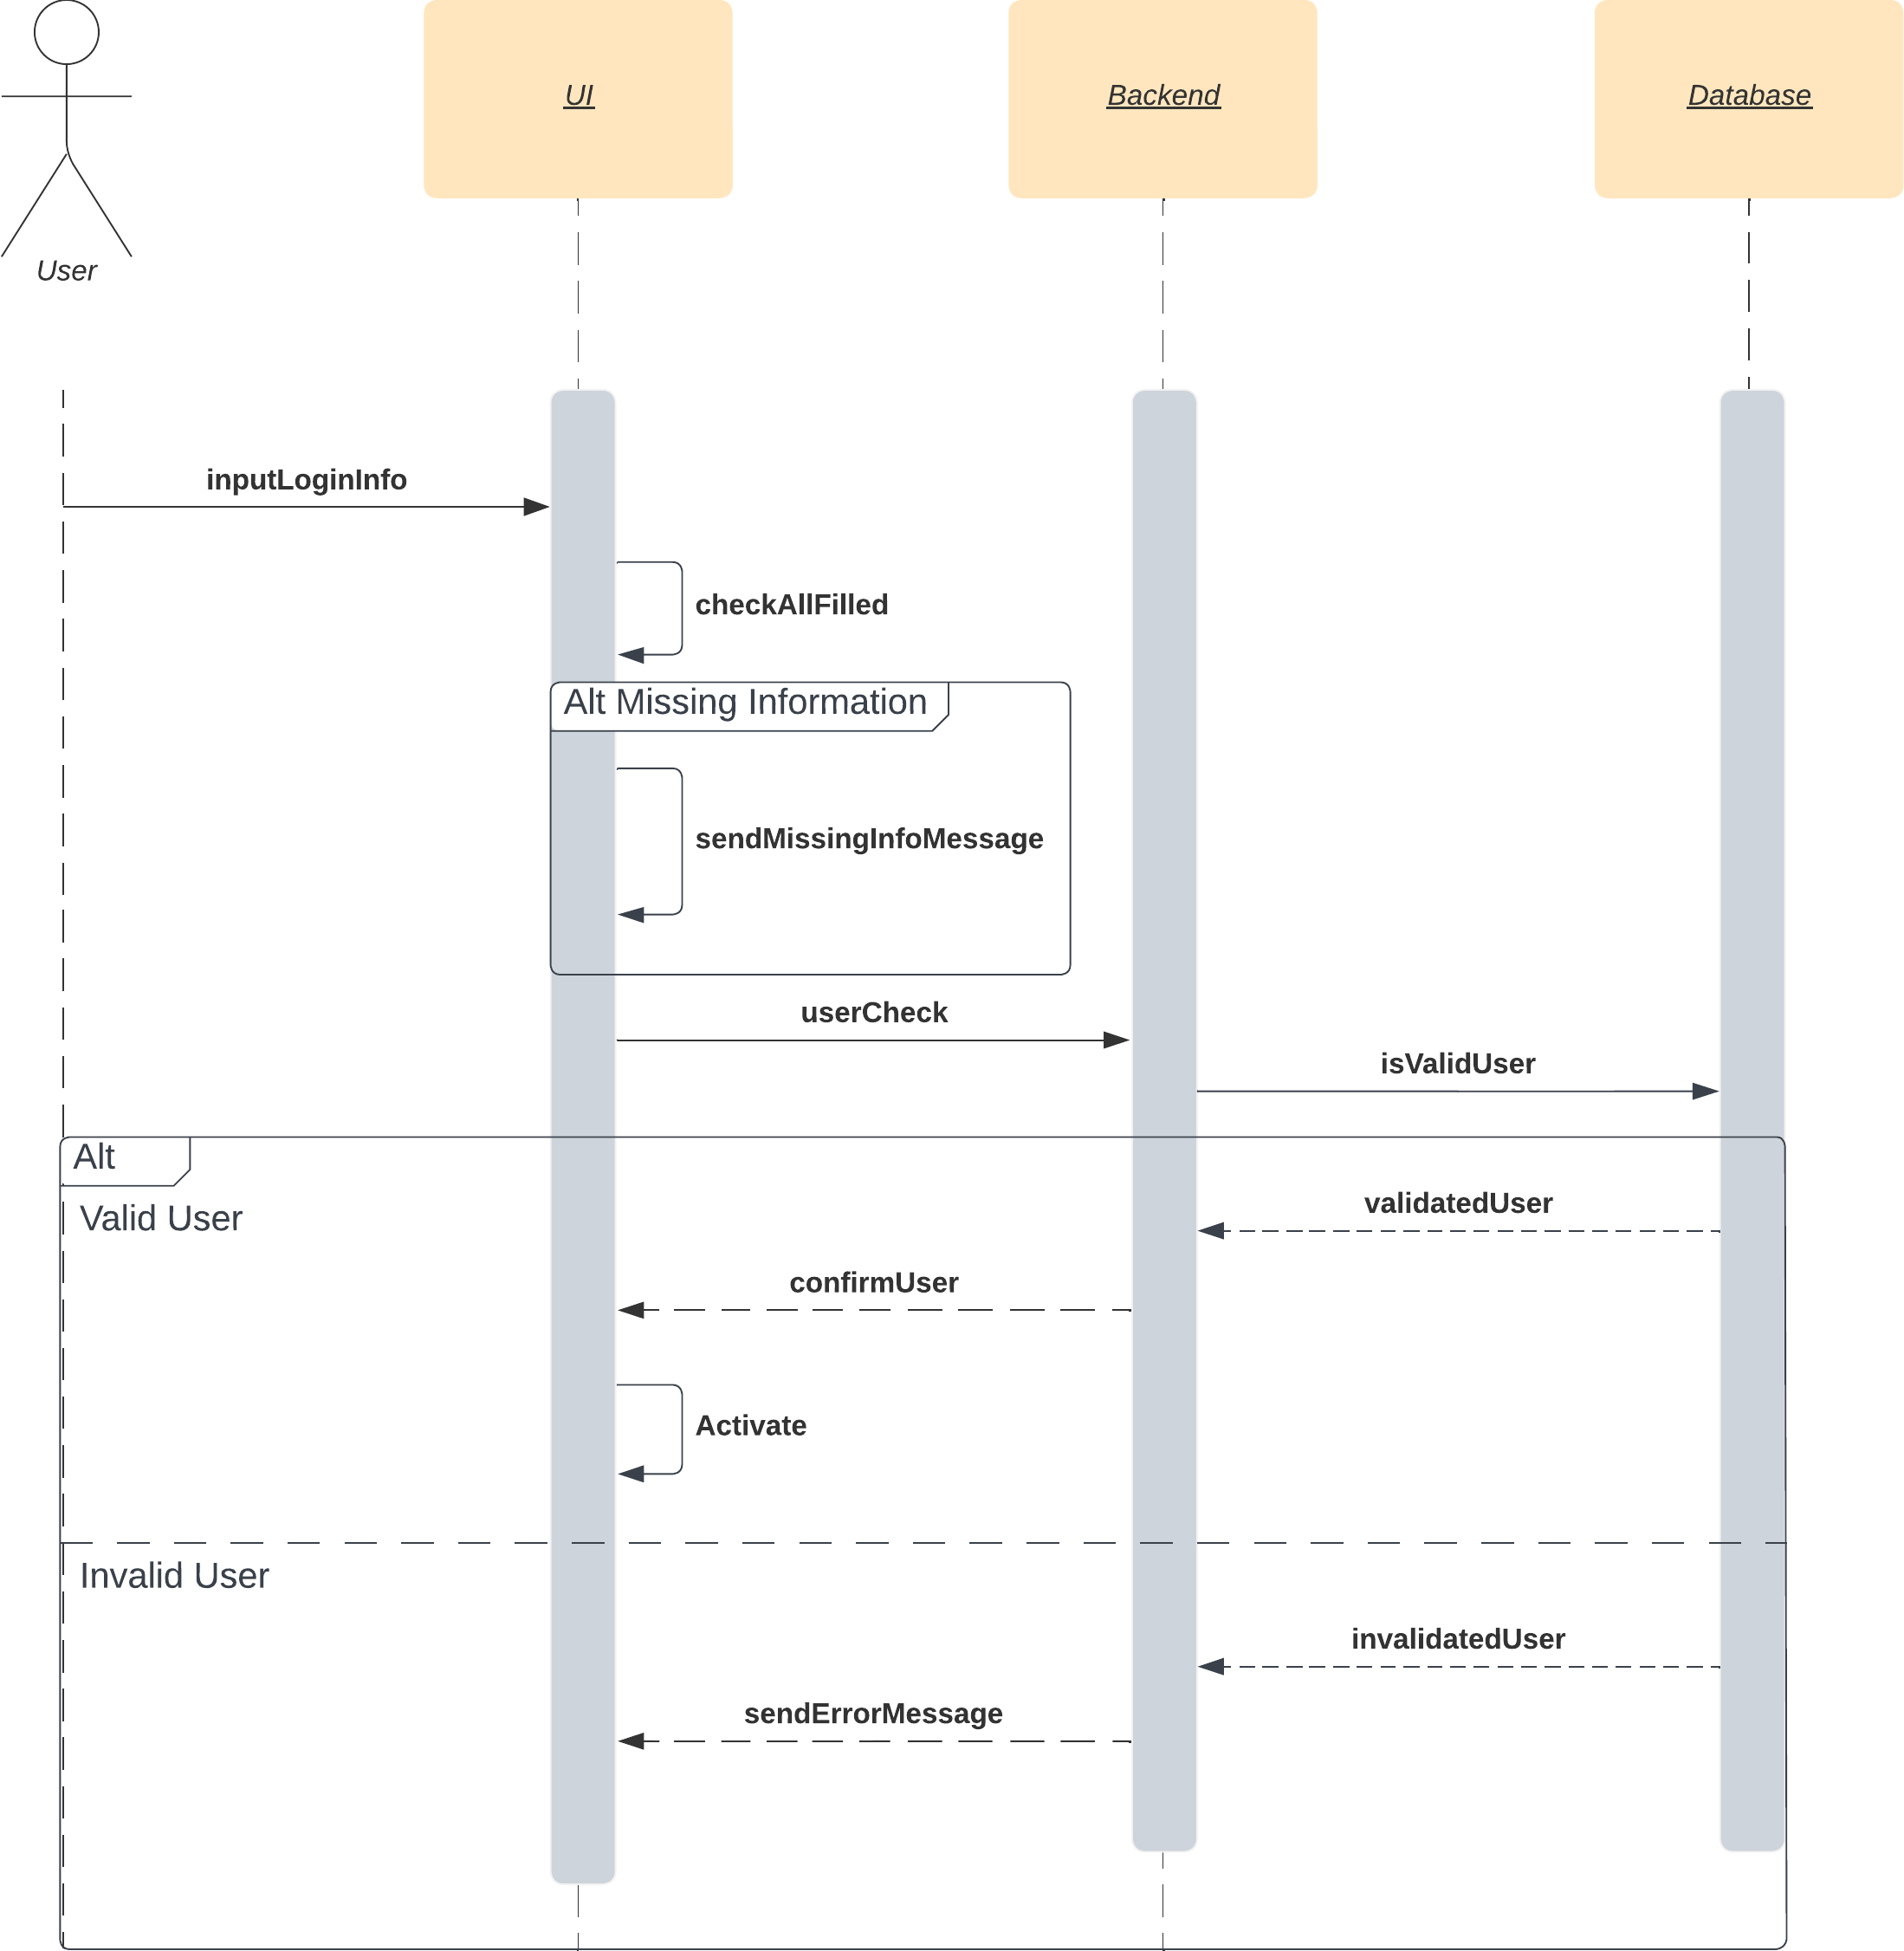
\includegraphics[width=15cm]{./login.png}}
    \caption{\centering Sequence diagram ของ login}\label{fig:Sequence diagram ของ login}
  \end{figure}

Sequence diagram สำหรับแสดงการทำงานของระบบขณะที่ผู้ใช้งานทำการเข้าสู่ระบบ 
โดยให้ผู้ใช้งานกรอกข้อมูลที่ใช้ในการเข้าสู่ระบบลงไปในหน้า log in ของ UI ตัว UI 
จะทำการตรวจข้อมูลที่ต้องการใช้ในการเข้าสู่ระบบว่ามีส่วนใดที่ขาด จากนั้นจึงส่งต่อให้ระบบ Backend 
ที่จะเรียกข้อมูลจาก Data base เพื่อตรวจสอบผู้ใช้งาน แล้วจึงเปิดหน้า UI ในกรณีที่ยืนยันได้ว่ามีผู้ใช้งานนั้นอยู่จริง


\newpage

\subsection{Registration}

  \begin{figure}[!h]\centering
    \setlength{\fboxrule}{0.5mm} % can define this in the preamble
    \setlength{\fboxsep}{0.5cm}
    \fbox{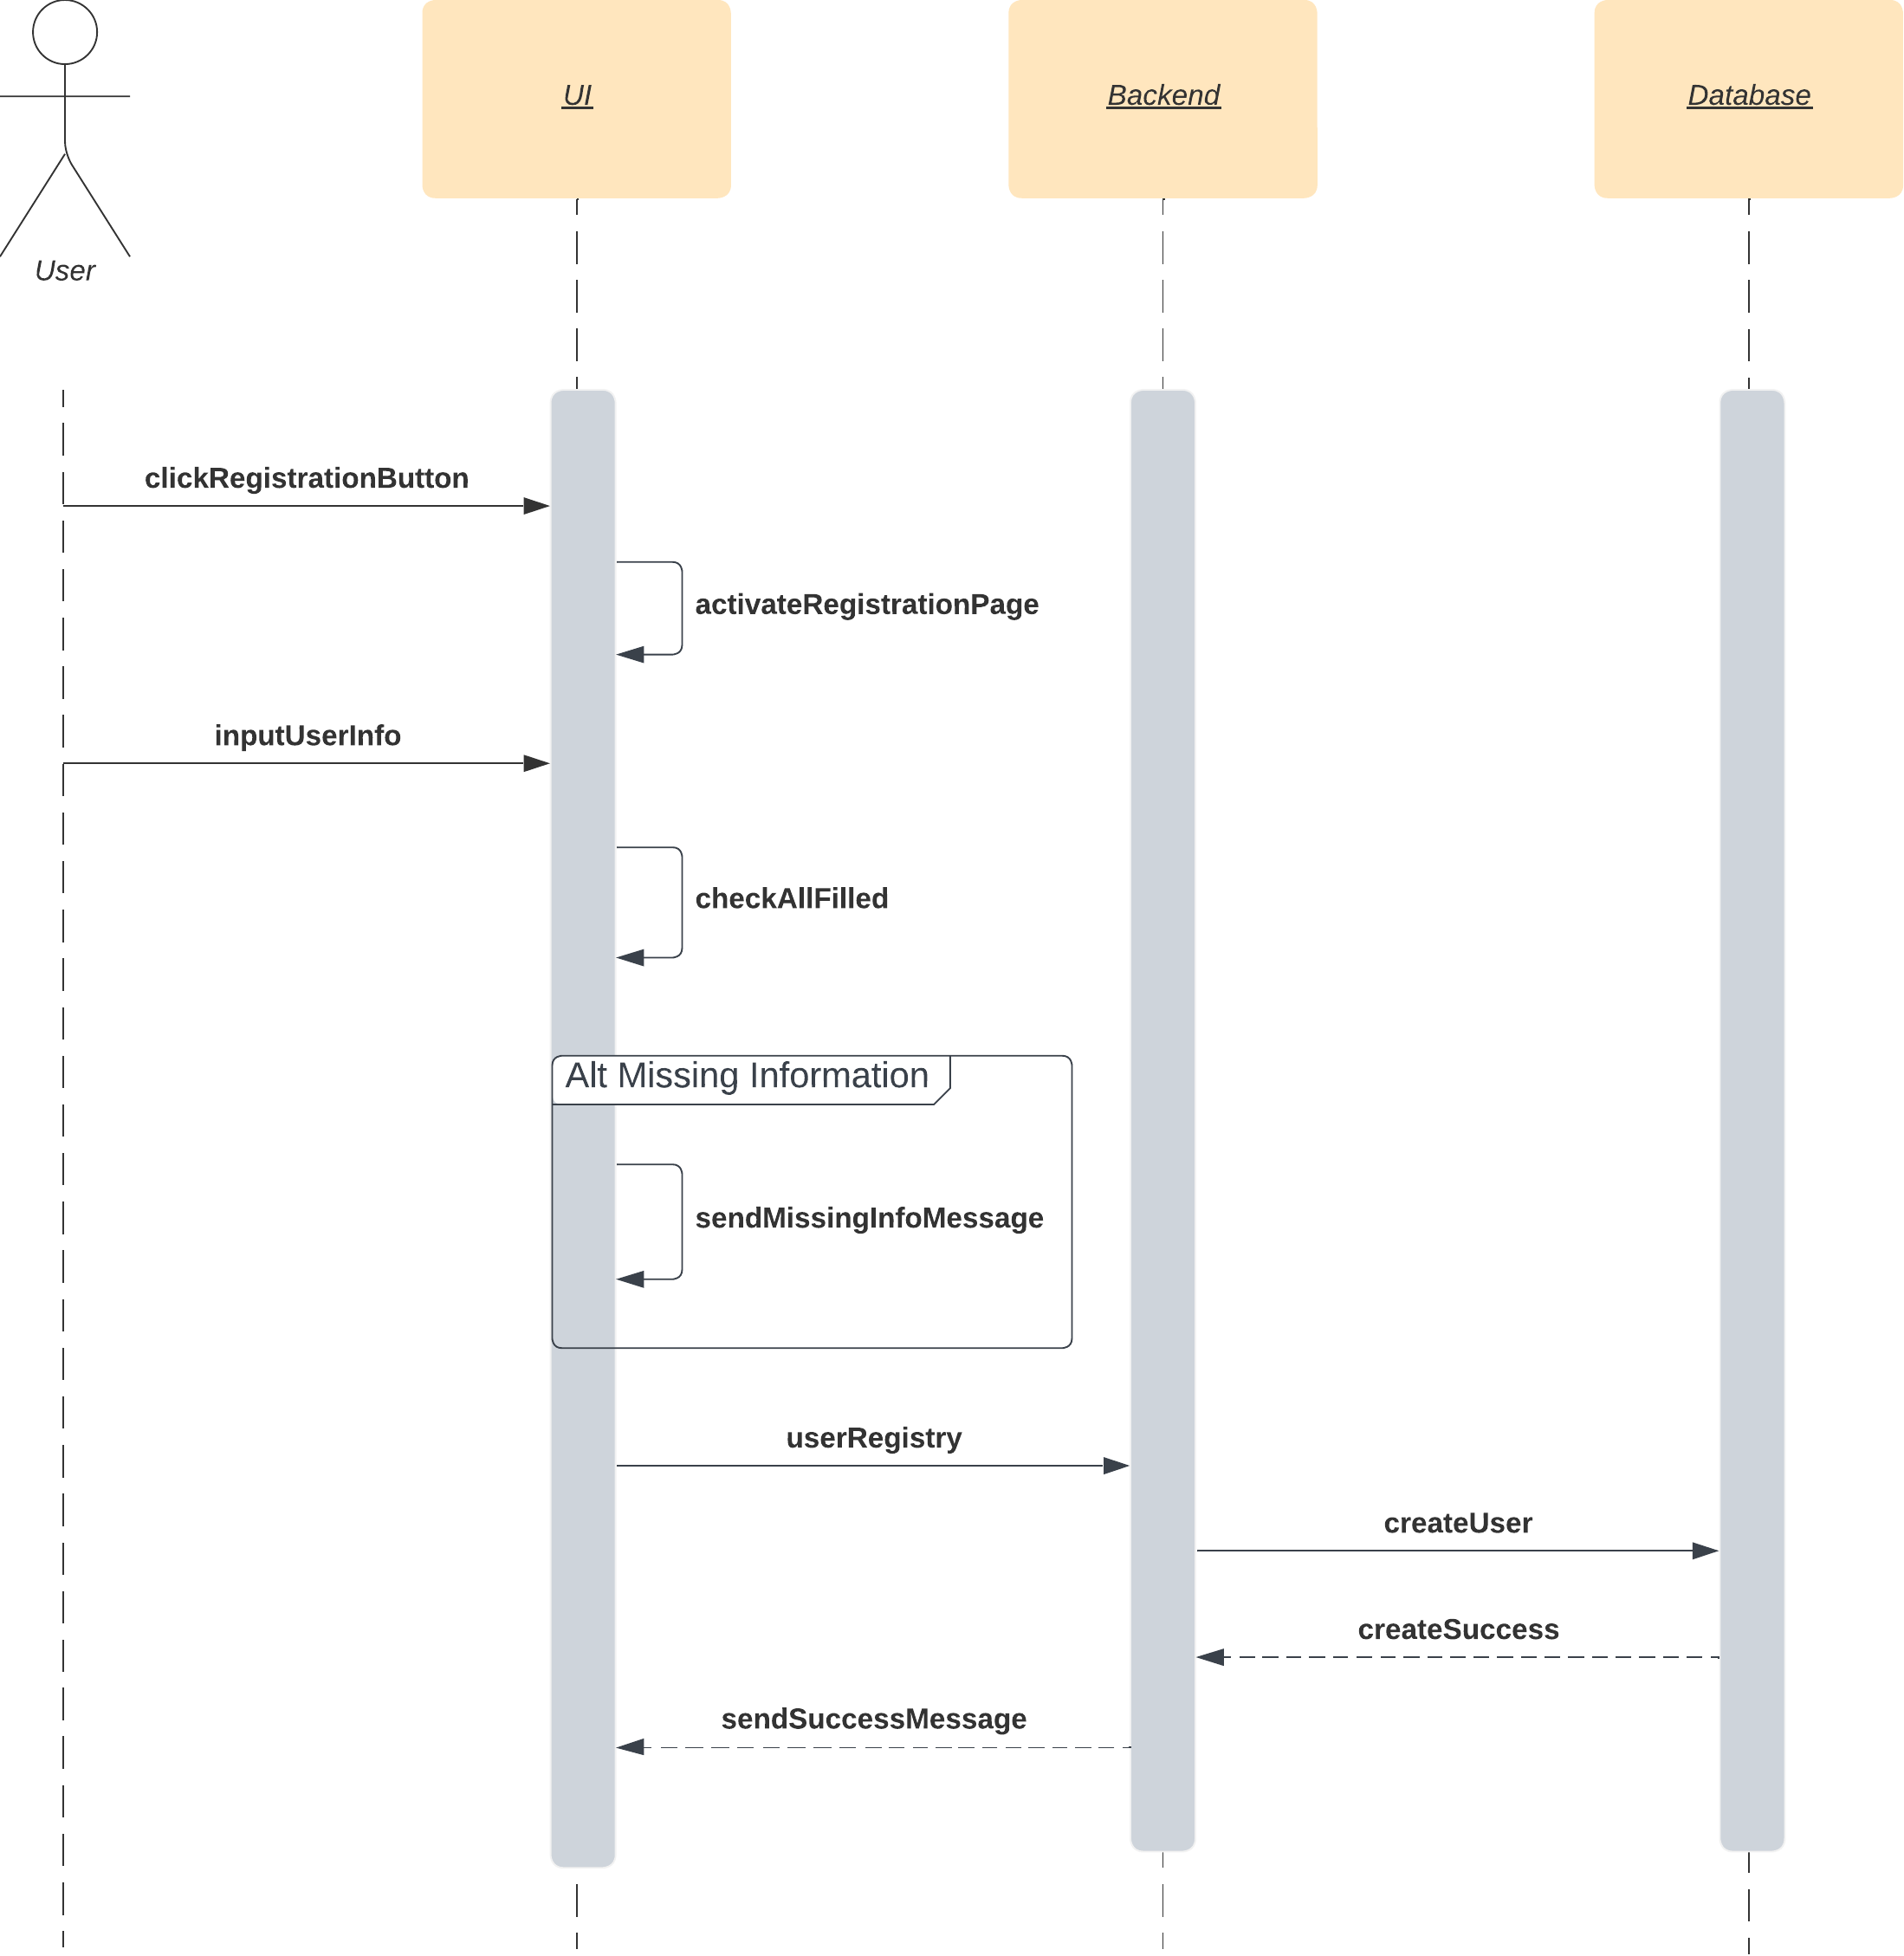
\includegraphics[width=15cm]{./regis.png}}
    \caption{\centering Registration}\label{fig:regis}
  \end{figure}

Sequence diagram สำหรับแสดงการทำงานของระบบขณะที่ผู้ใช้งานทำการสมัครเข้าใช้งาน โดยหลังจากผู้ใช้งานกดตุ่มเพื่อสมัครใช้งานแล้วระบบ UI จะขึ้นหน้าให้กรอกข้อมูลที่ใช้ในการสมัครเข้าใช้งาน ตัว UI จะทำการตรวจข้อมูลที่ต้องการใช้ในการเข้าสู่ระบบว่ามีส่วนใดที่ขาด จากนั้นจึงส่งต่อให้ระบบ Backend ซึ่งจะส่งข้อมูลไปบันทึกที่ Data base  แล้วระบบจะส่งข้อความยืนยันการสมัครเข้าใช้งานกลับขึ้นไปหาผู้ใช้งานที่สมัคร


\newpage


\subsection{Logout}

  \begin{figure}[!h]\centering
    \setlength{\fboxrule}{0.5mm} % can define this in the preamble
    \setlength{\fboxsep}{0.5cm}
    \fbox{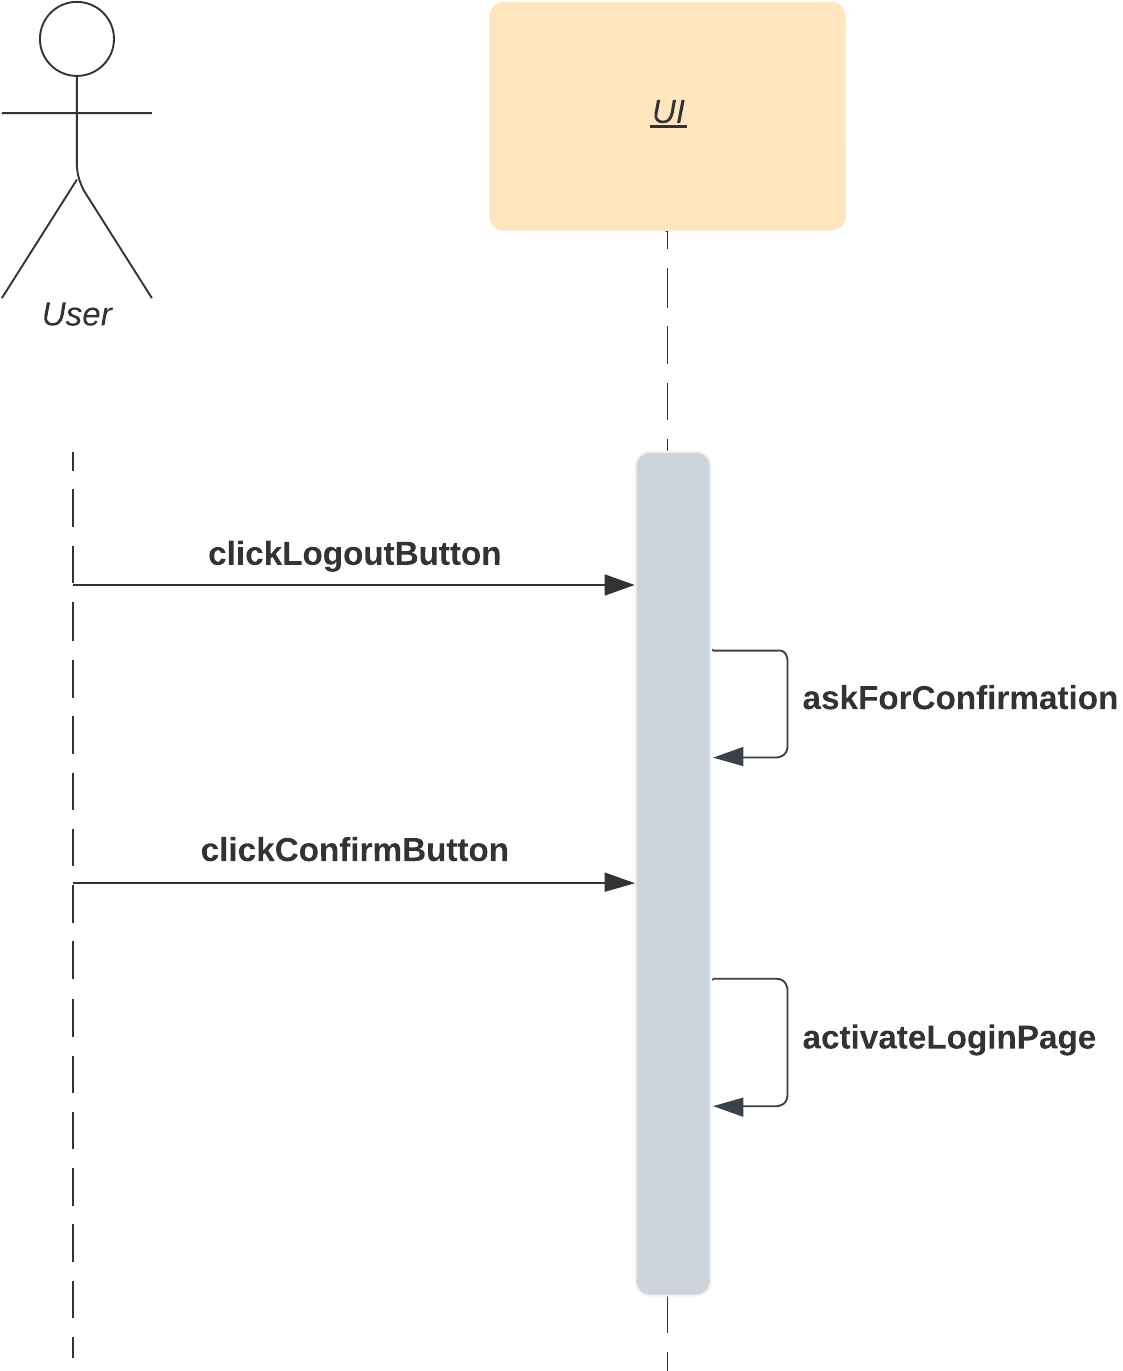
\includegraphics[width=15cm]{./logout.png}}
    \caption{Logout}\label{fig:logout}
  \end{figure}

Sequence diagram สำหรับแสดงการทำงานของระบบขณะที่ผู้ใช้งานออกจากระบบ โดยหลังจากผู้ใช้งานกดปุมออกจากระบบ UI จะถามการยืนยันการออกจากระบบซึ่งหลังจากผู้ใช้งานกดยืนยันแล้วระบบจะพาผู้ใช้ไปยังหน้าเข้าสู่ระบบอีกครั้ง

\newpage

\subsection{Search Event}

  \begin{figure}[!h]\centering
    \setlength{\fboxrule}{0.5mm} % can define this in the preamble
    \setlength{\fboxsep}{0.5cm}
    \fbox{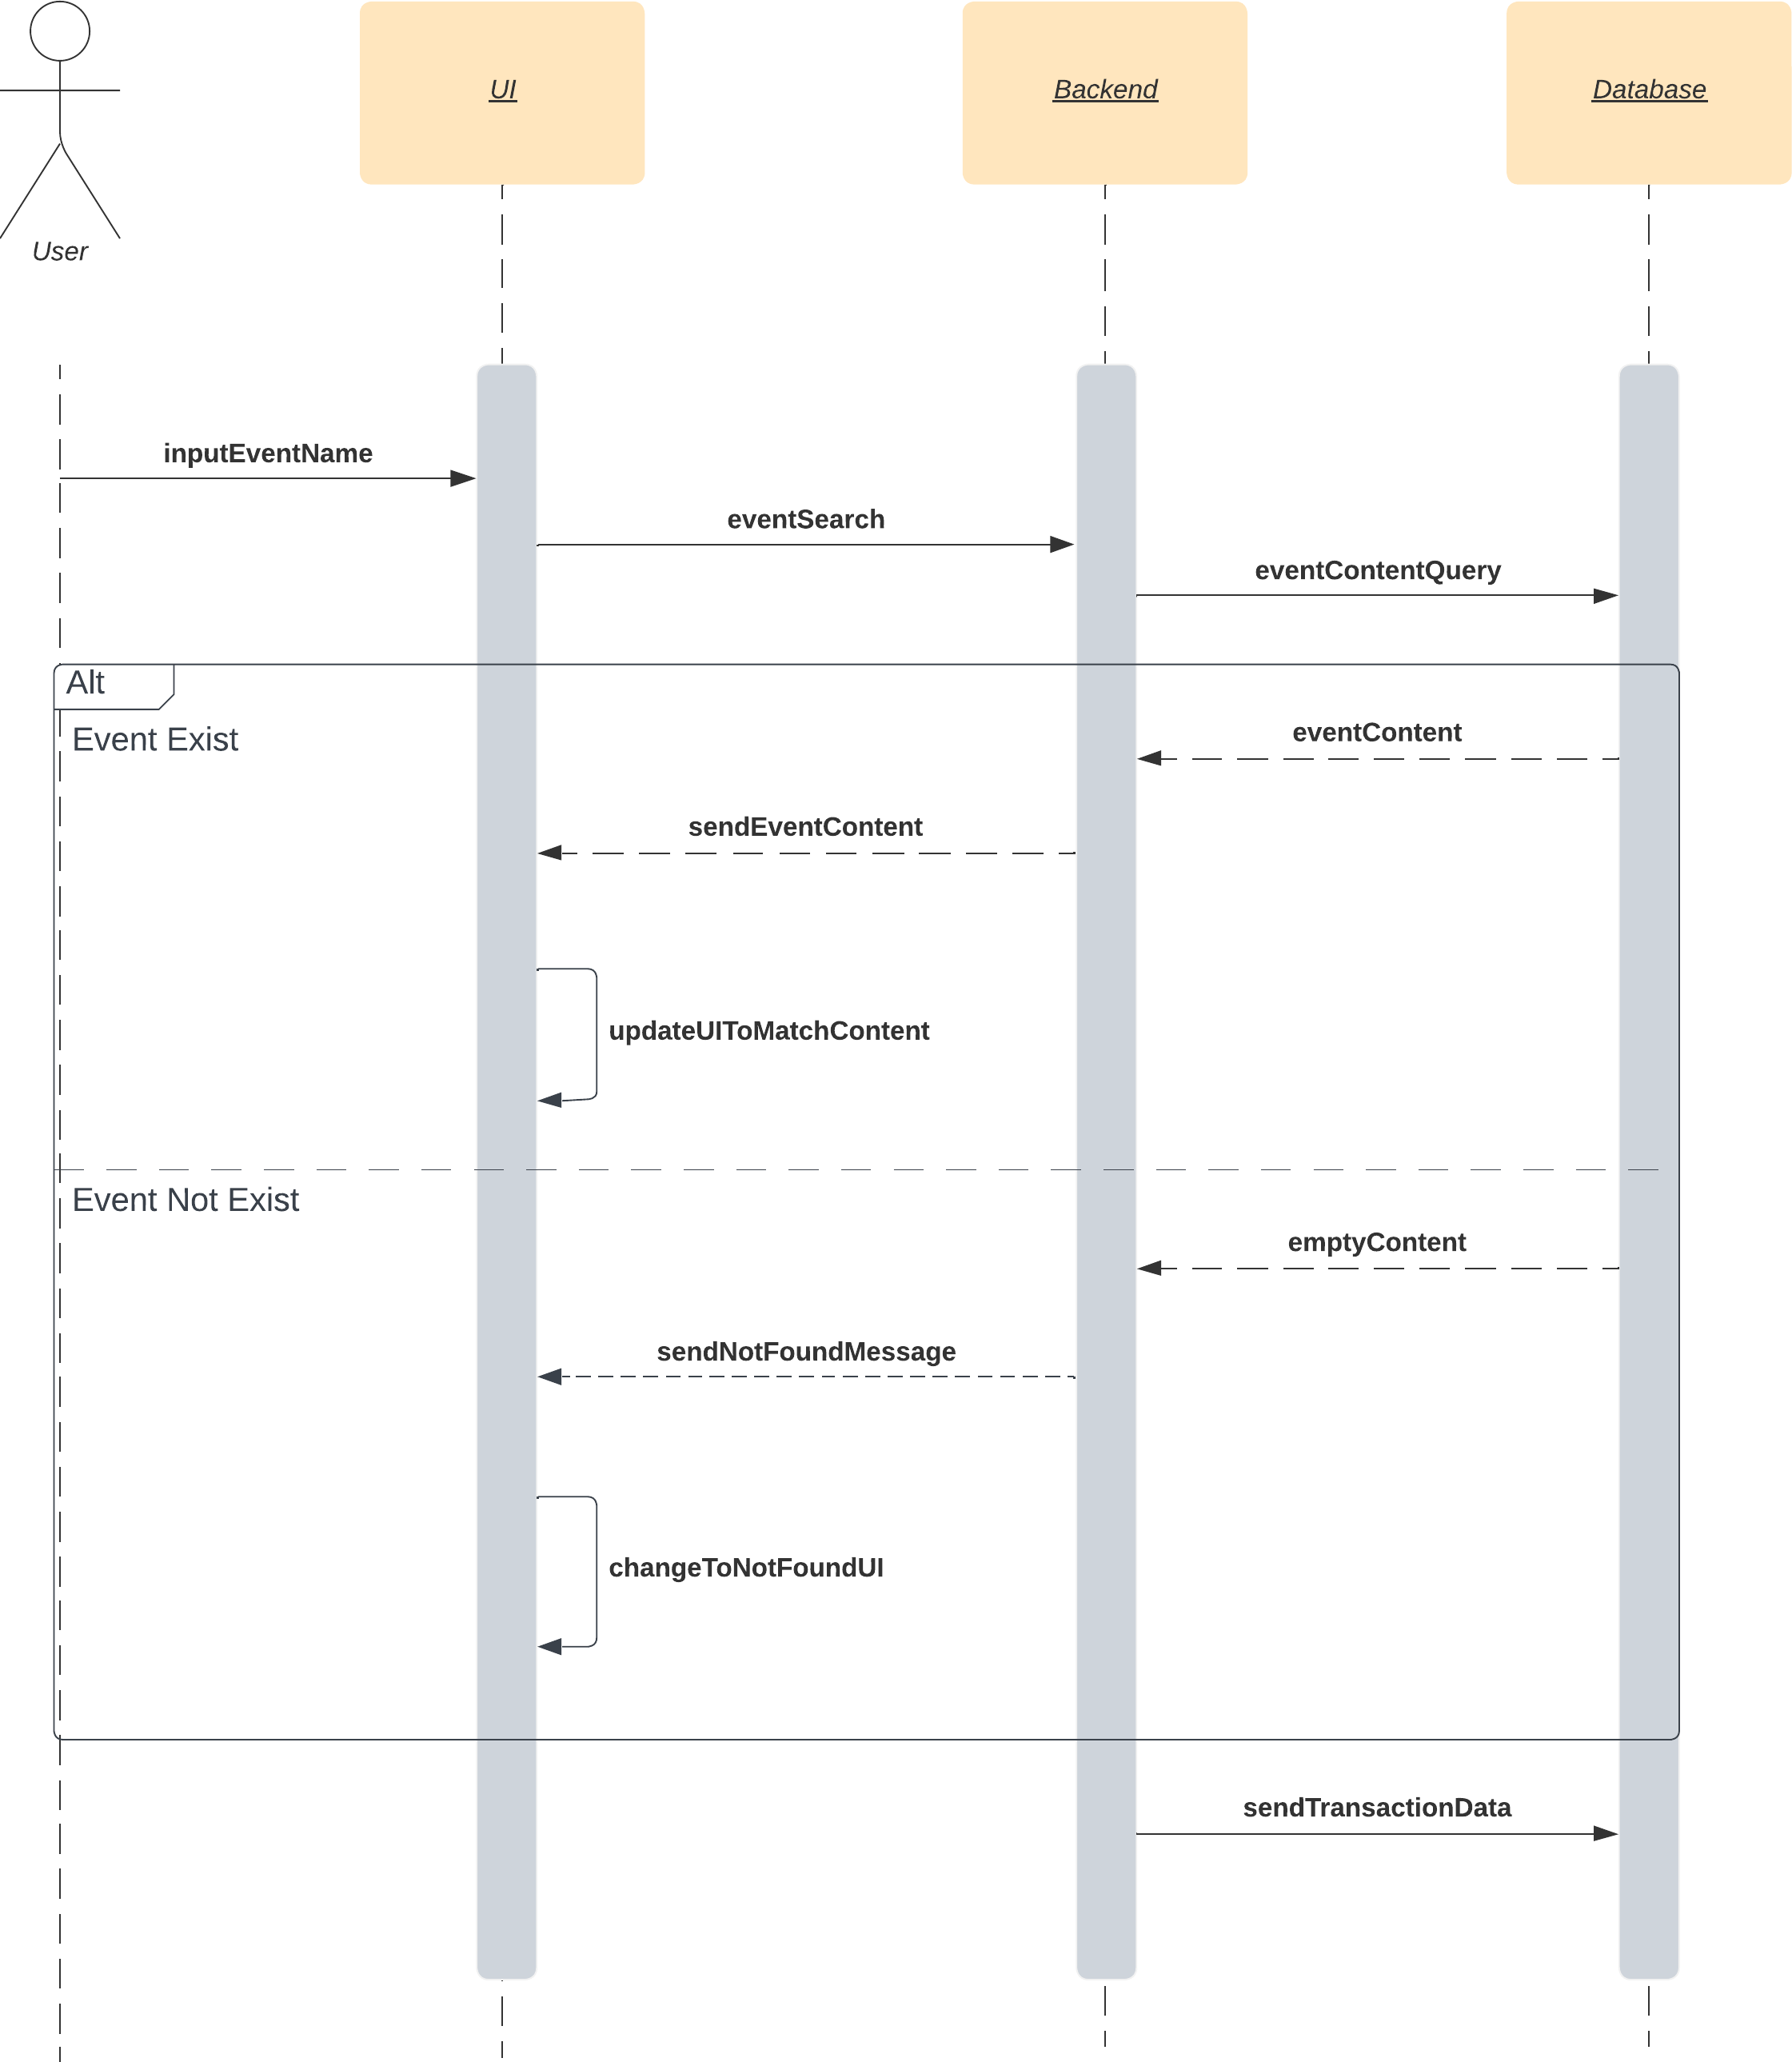
\includegraphics[width=15cm]{./searchev.png}}
    \caption{Search Event}\label{fig:Search Event}
  \end{figure}

Sequence diagram สำหรับแสดงการทำงานของระบบขณะที่ผู้ใช้งานทำการค้นหากิจกรรม โดย UI จะรับสิ่งที่ผู้ใช้งานต้องการค้นหาส่งไปหา Backend เพื่อให้ Backend ค้นหาข้อมูลที่เก็บไว้จาก Data base หากพบเจอจะส่งข้อมูลกลับไปหาข้อผู้ใช้งาน หากไม่เจอจะแสดงข้อความว่าไม่พบกิจกรรม และส่งข้อมูลการใช้งานไปเก็บยัง Data base

\newpage

\subsection{Select and join event}

  \begin{figure}[!h]\centering
    \setlength{\fboxrule}{0.5mm} % can define this in the preamble
    \setlength{\fboxsep}{0.5cm}
    \fbox{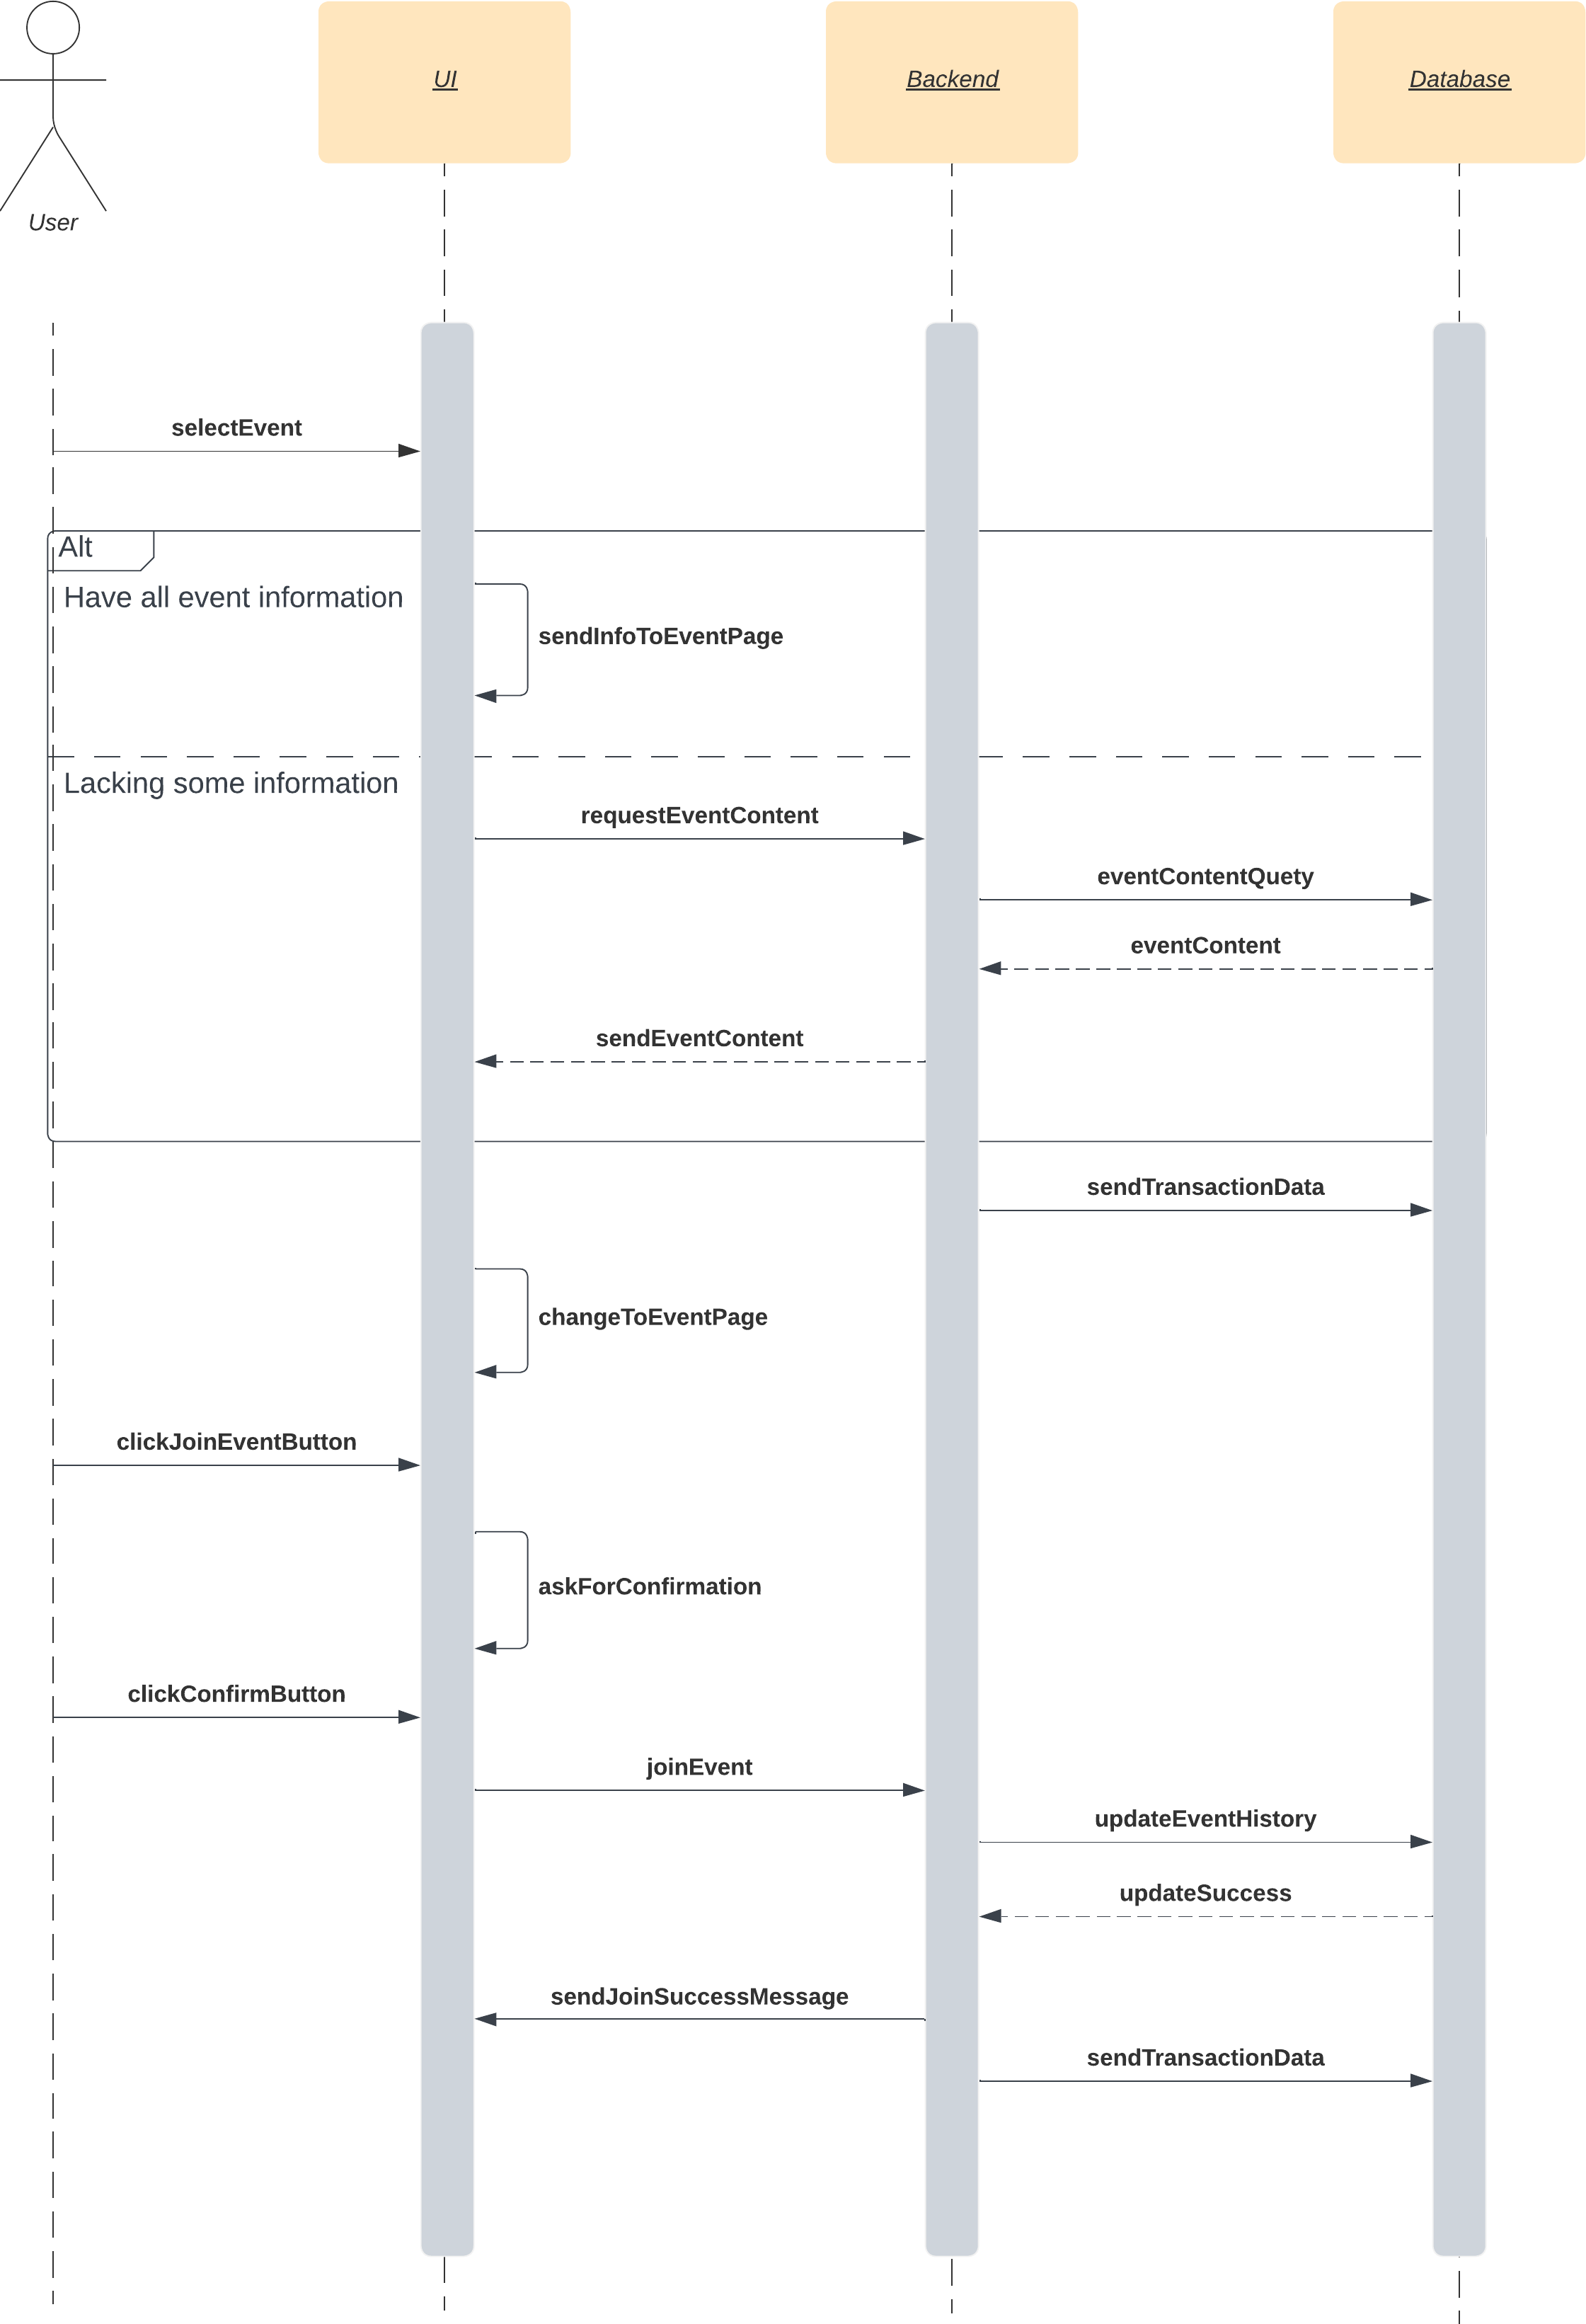
\includegraphics[width=13cm]{./selectandjoin.png}}
    \caption{Select and join event}\label{fig:Select and join event}
  \end{figure}

Sequence diagram สำหรับแสดงการทำงานของระบบขณะที่ผู้ใช้งานทำการเข้าไปอ่านรายละเอียดของกิจกรรม โดย UI จะแสดงข้อมูลหากมีข้อมูลของกิจกรรมนั้นอยู่แล้ว หากไม่มีจะส่งคำขอให้ Back end ดึงข้อมูลจาก Data base ให้ หากผู้ใช้งานทำการกดเข้าร่วมกิจกรรม UI จะทำการขอการยืนยันจากผู้ใช้งานอีกครั้ง ซึ่งหากกดยืนยันแล้วก็จะส่งข้อมูลการเข้าร่วมไปให้ Backend จัดเก็บใน Data base 

\newpage

\subsection{Event evaluation}

  \begin{figure}[!h]\centering
    \setlength{\fboxrule}{0.5mm} % can define this in the preamble
    \setlength{\fboxsep}{0.5cm}
    \fbox{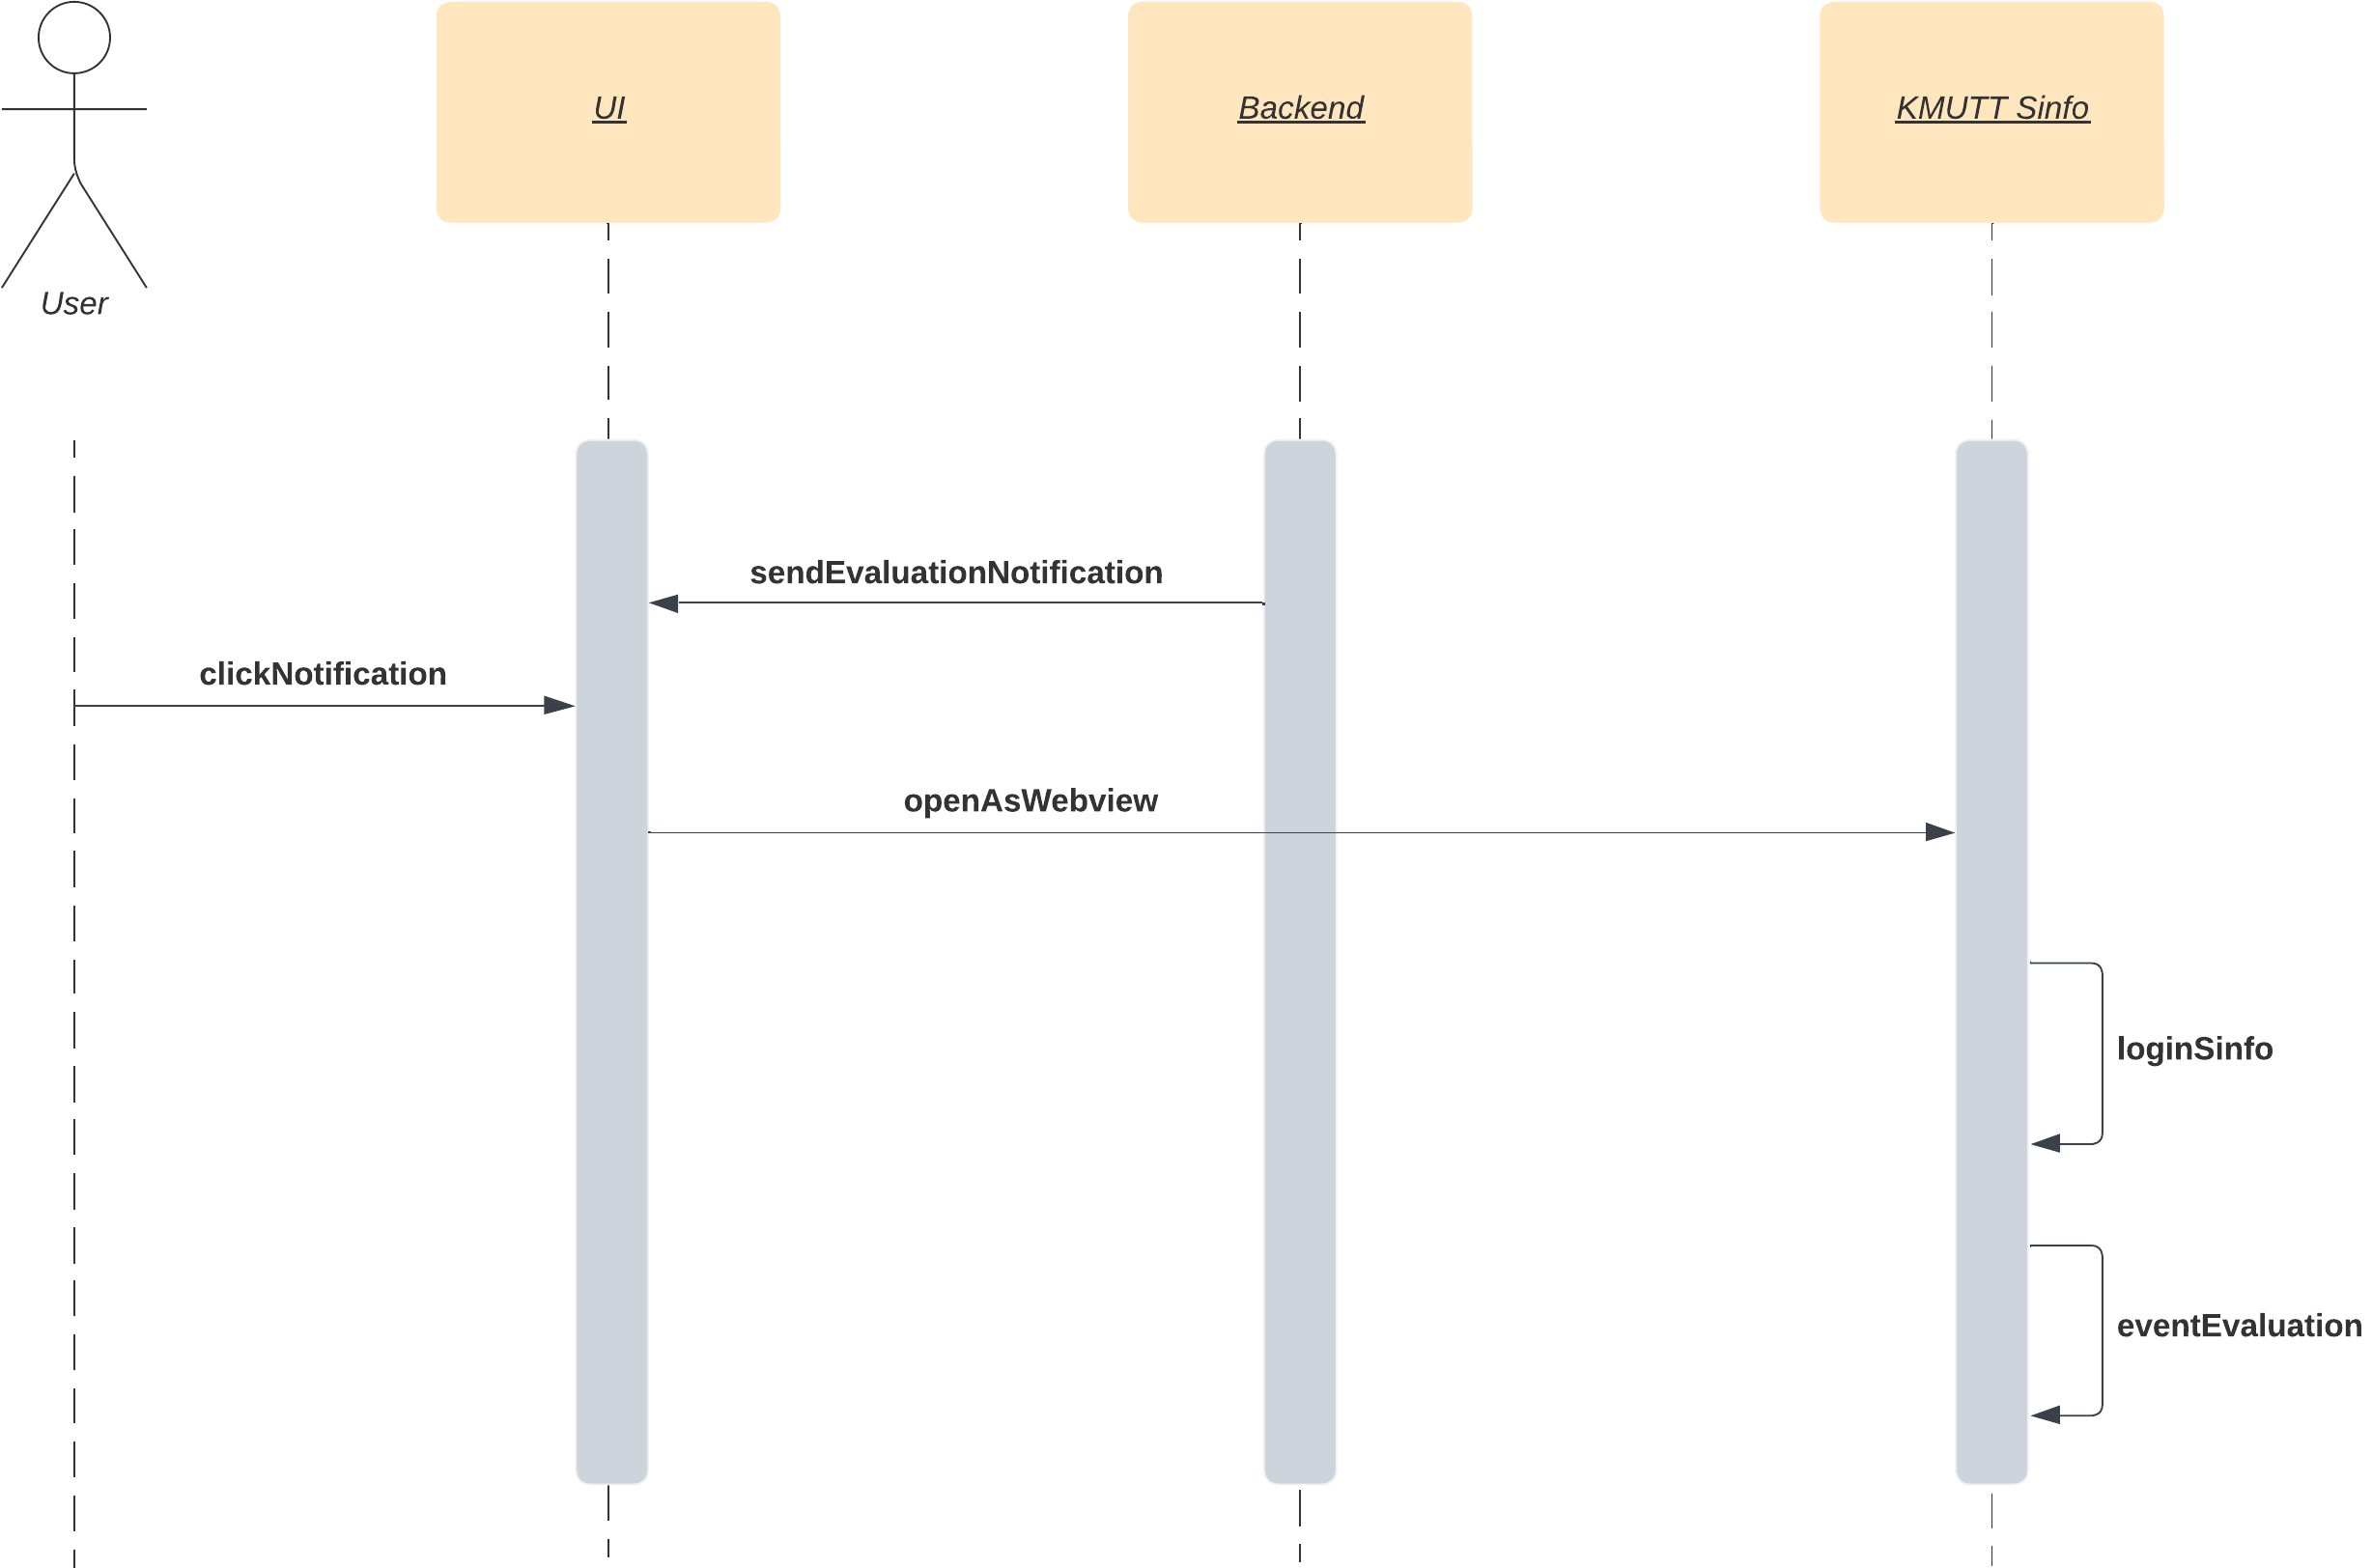
\includegraphics[width=15cm]{./evaluate.png}}
    \caption{Event evaluation}\label{fig:Event evaluation}
  \end{figure}

  Sequence diagram สำหรับแสดงการทำงานของระบบแจ้งเตือนกิจกรรมชมรม โดย Backend จะส่งคำเตือนเข้ามาหา UI เพื่อที่จะแจ้งถึงกิจกรรมที่ชมรมจัดขึ้น เมื่อผู้ใช้งานกดเข้าอ่านรายละเอียดกิจกรรมแล้ว UI จะขอให้ Backend หาข้อมูลกิจกรรมจาก Data base มาแสดงให้ผู้ใช้งาน และส่งข้อมูลการใช้งานไปเก็บยัง Data base

\newpage

\subsection{Notification about event from club}

  \begin{figure}[!h]\centering
    \setlength{\fboxrule}{0.5mm} % can define this in the preamble
    \setlength{\fboxsep}{0.5cm}
    \fbox{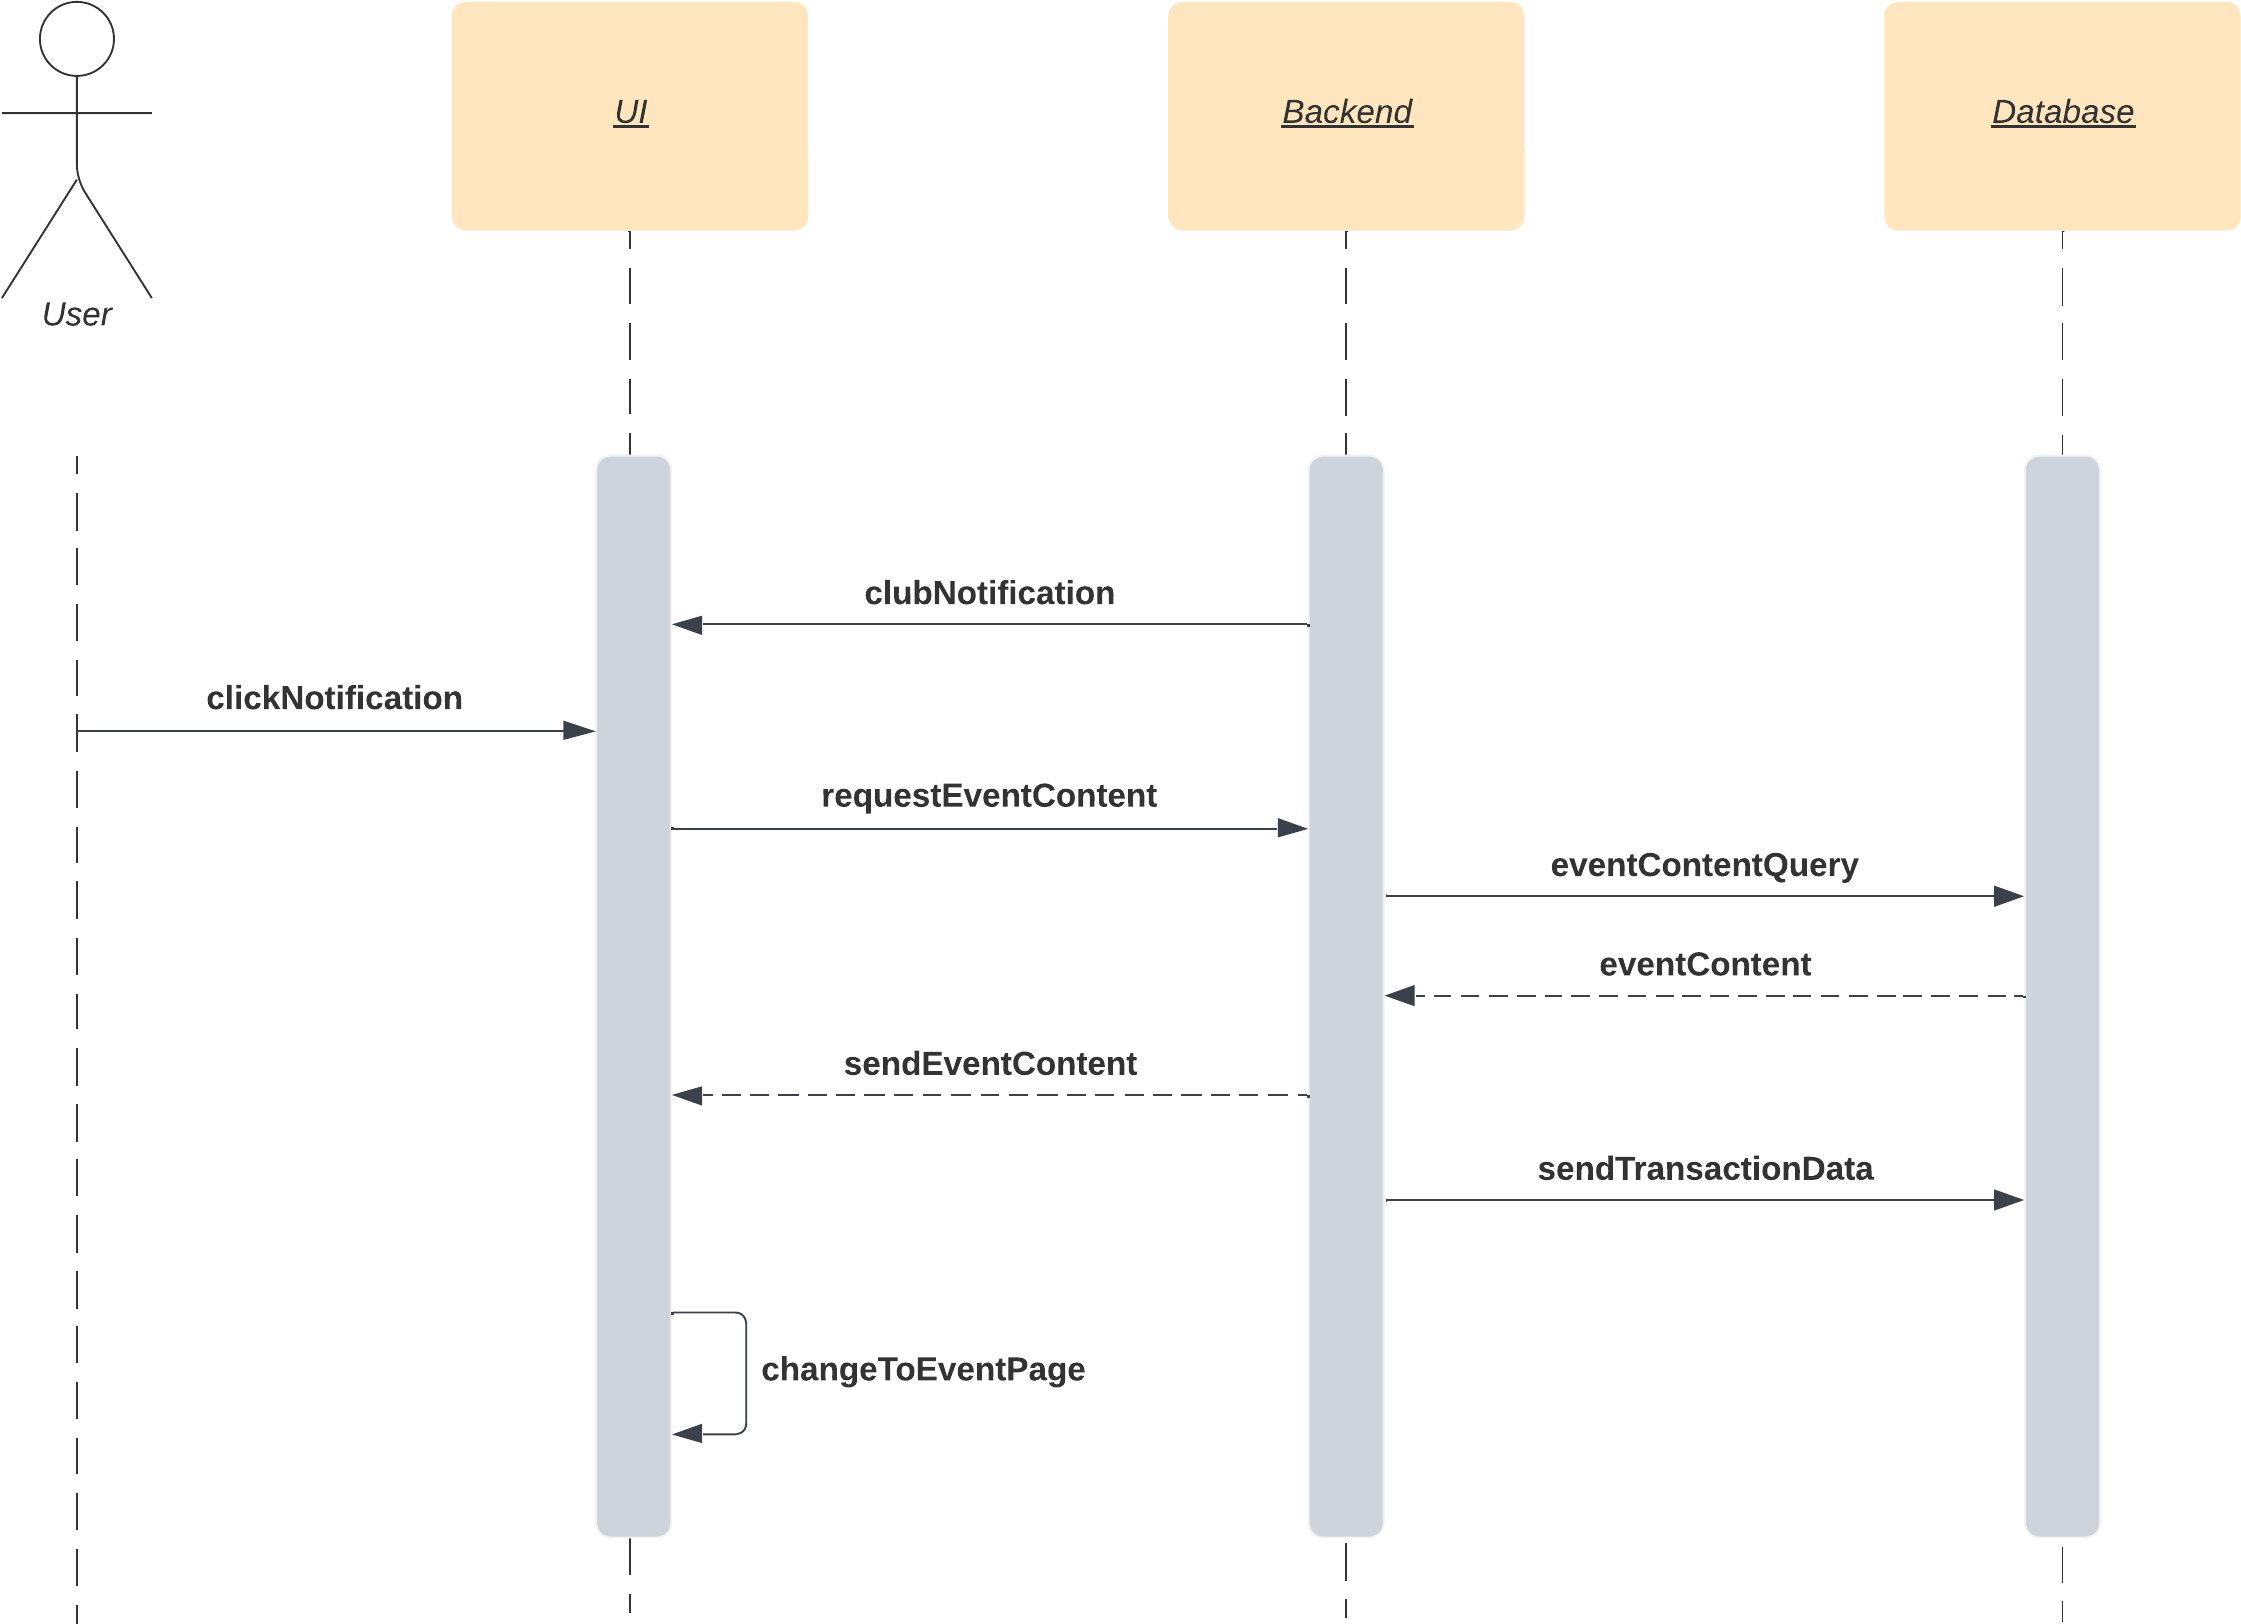
\includegraphics[width=15cm]{./Noti.png}}
    \caption{Notification about event from club}\label{fig:Notification about event from club}
  \end{figure}

Sequence diagram สำหรับแสดงการทำงานของระบบแจ้งเตือนการประเมินกิจกรรม โดย Backend จะส่งคำเตือนเข้ามาหา UI เพื่อที่จะแจ้งเตือนการประเมินกิจกรรม เมื่อผู้ใช้งานกดเข้าลิงค์ประเมินกิจกรรมแล้วจะเปิดหน้าต่างเพื่อประเมินกิจกรรมให้

\newpage

\subsection{Seacrh club}

  \begin{figure}[!h]\centering
    \setlength{\fboxrule}{0.5mm} % can define this in the preamble
    \setlength{\fboxsep}{0.5cm}
    \fbox{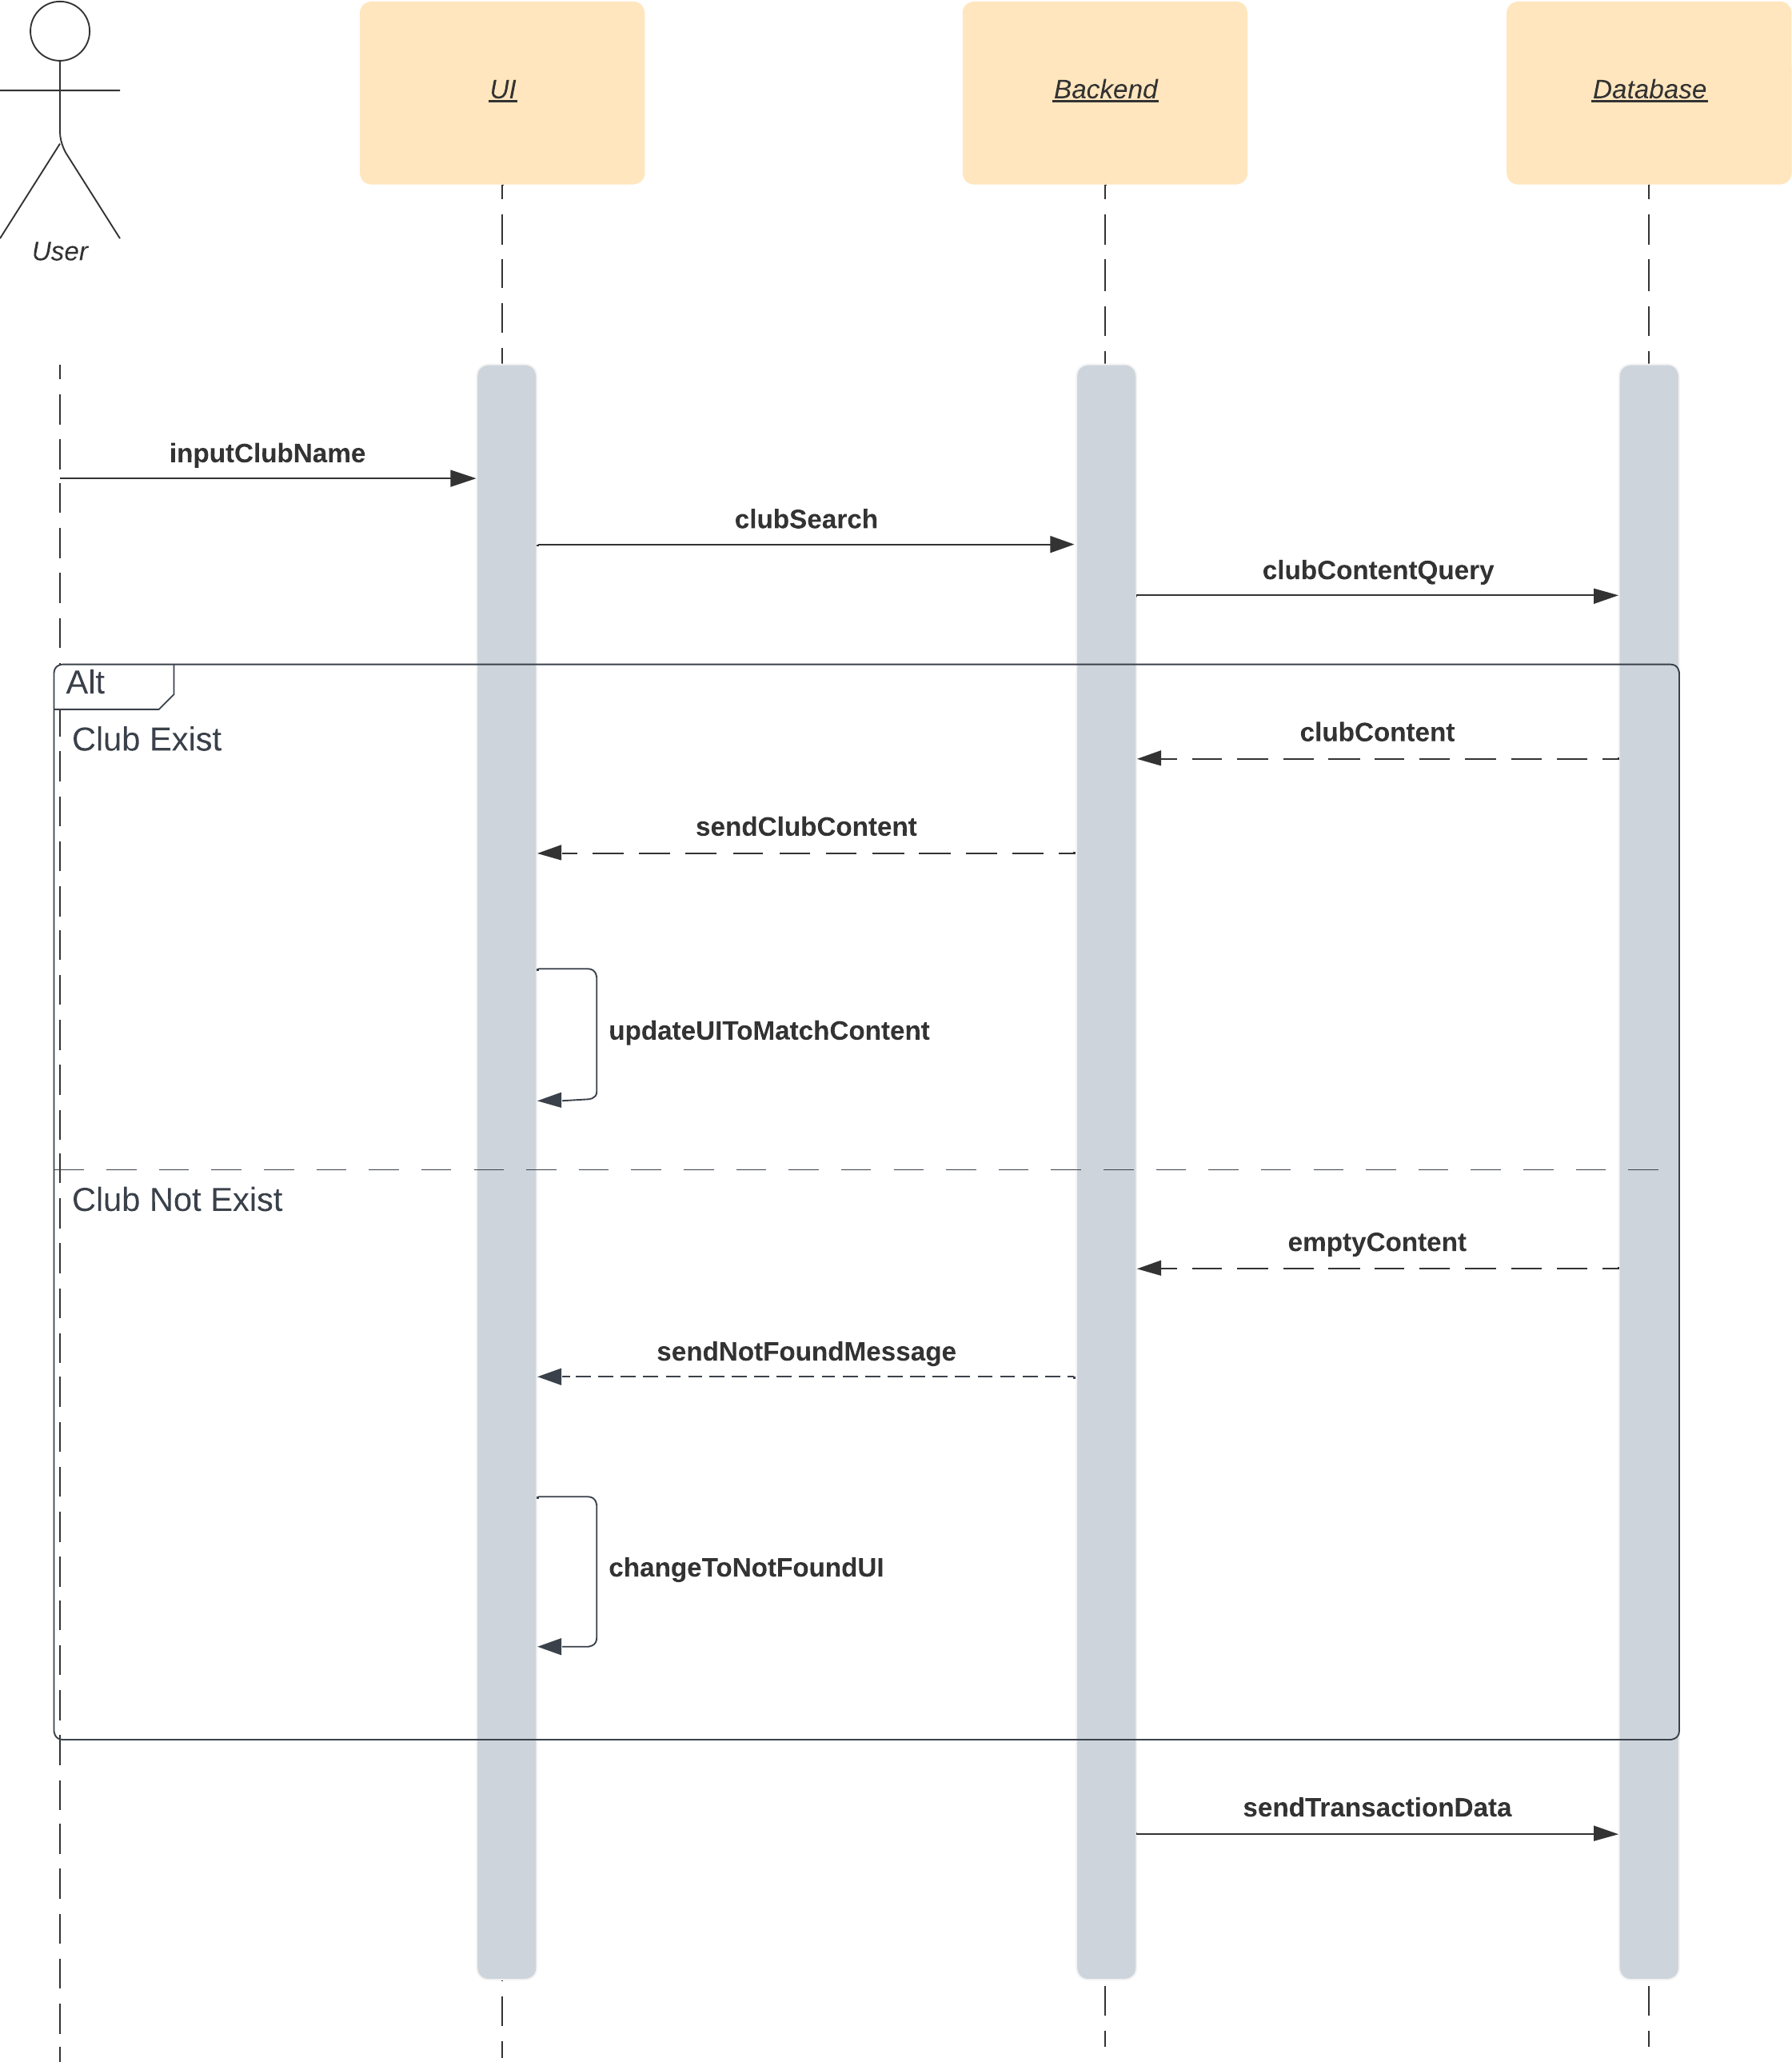
\includegraphics[width=15cm]{./searchclub.png}}
    \caption{Seacrh club}\label{fig:Seacrh club}
  \end{figure}

Sequence diagram สำหรับแสดงการทำงานของระบบขณะที่ผู้ใช้งานทำการค้นหาชมรมโดย UI จะรับสิ่งที่ผู้ใช้งานต้องการค้นหาส่งไปหา Backend เพื่อให้ Backend ค้นหาข้อมูลที่เก็บไว้จาก Data base หากพบเจอจะส่งข้อมูลกลับไปหาข้อผู้ใช้งาน หากไม่เจอจะแสดงข้อความว่าไม่พบกิจกรรม และส่งข้อมูลการใช้งานไปเก็บยัง Data base

\newpage

\subsection{Select and join club}

  \begin{figure}[!h]\centering
    \setlength{\fboxrule}{0.5mm} % can define this in the preamble
    \setlength{\fboxsep}{0.5cm}
    \fbox{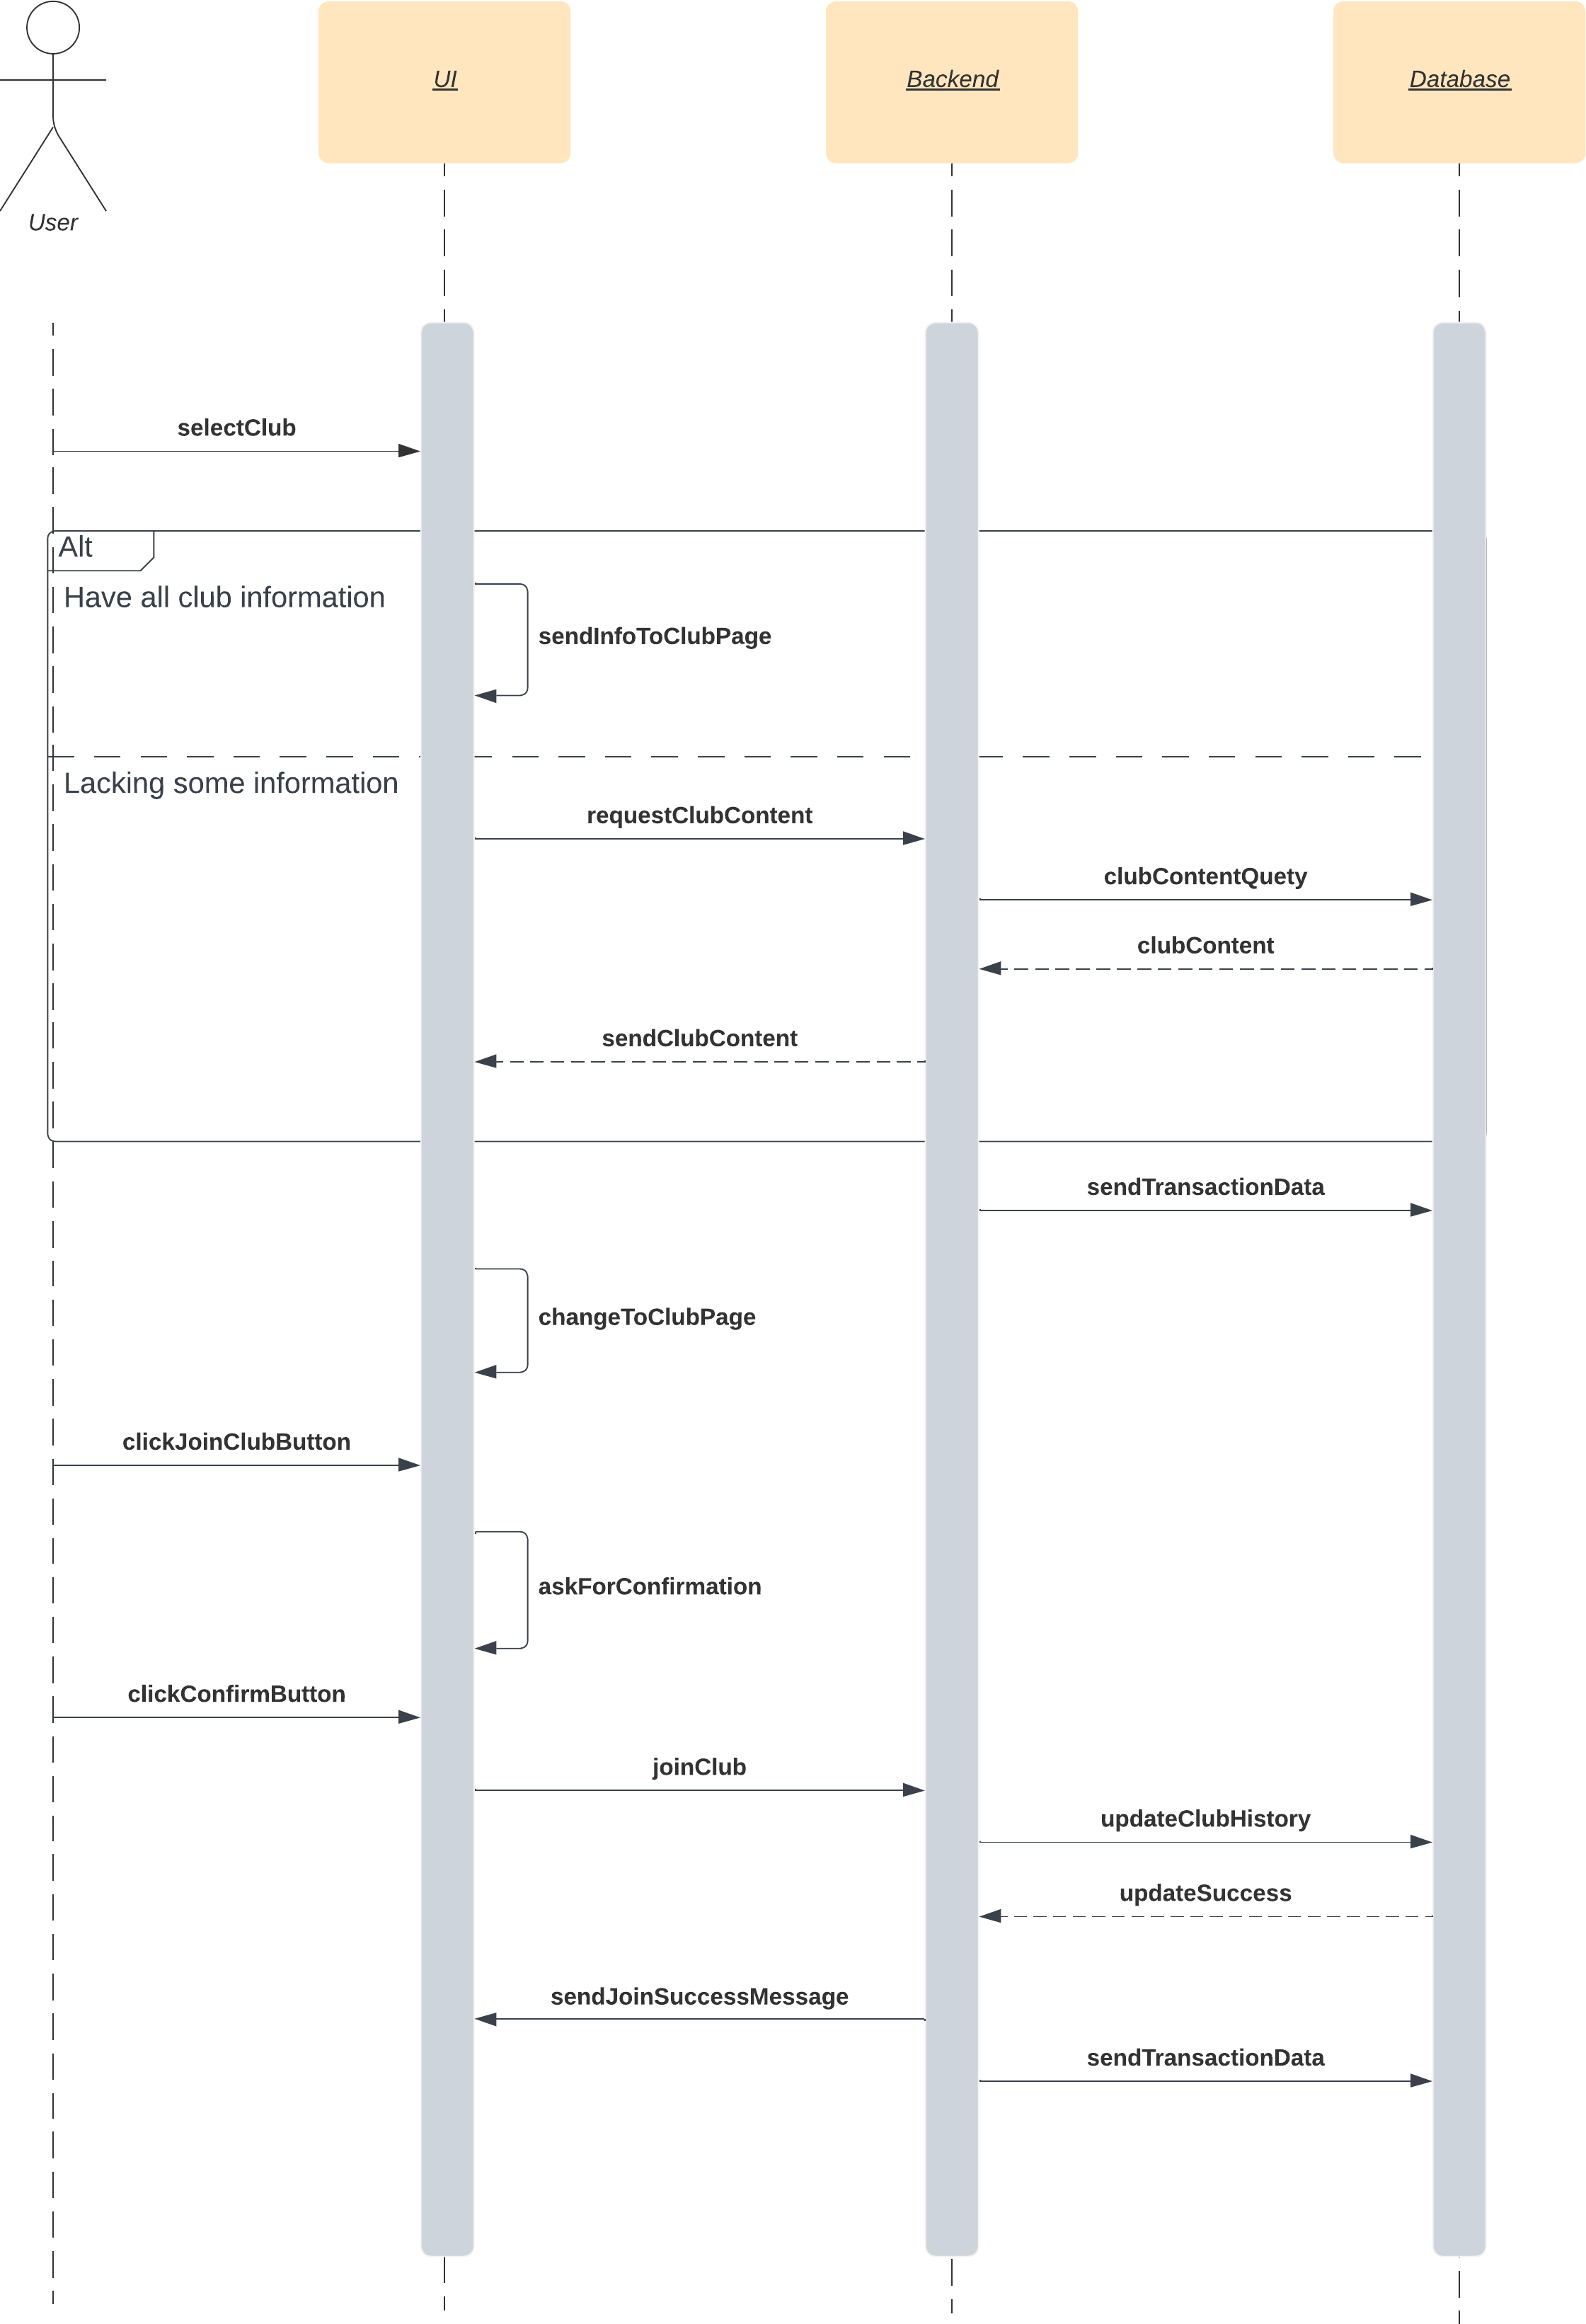
\includegraphics[width=13cm]{./selectandjoinclub.png}}
    \caption{Select and join club}\label{fig:Select and join club}
  \end{figure}

Sequence diagram สำหรับแสดงการทำงานของระบบขณะที่ผู้ใช้งานทำการเข้าไปอ่านรายละเอียดของชมรม โดย UI จะแสดงข้อมูลหากมีข้อมูลของกิจกรรมนั้นอยู่แล้ว หากไม่มีจะส่งคำขอให้ Back end ดึงข้อมูลจาก Data base ให้ หากผู้ใช้งานทำการกดเข้าร่วมกิจกรรม UI จะทำการขอการยืนยันจากผู้ใช้งานอีกครั้ง ซึ่งหากกดยืนยันแล้วก็จะส่งข้อมูลการเข้าร่วมไปให้ Backend จัดเก็บใน Data base

\newpage

\subsection{Club resignation}

  \begin{figure}[!h]\centering
    \setlength{\fboxrule}{0.5mm} % can define this in the preamble
    \setlength{\fboxsep}{0.5cm}
    \fbox{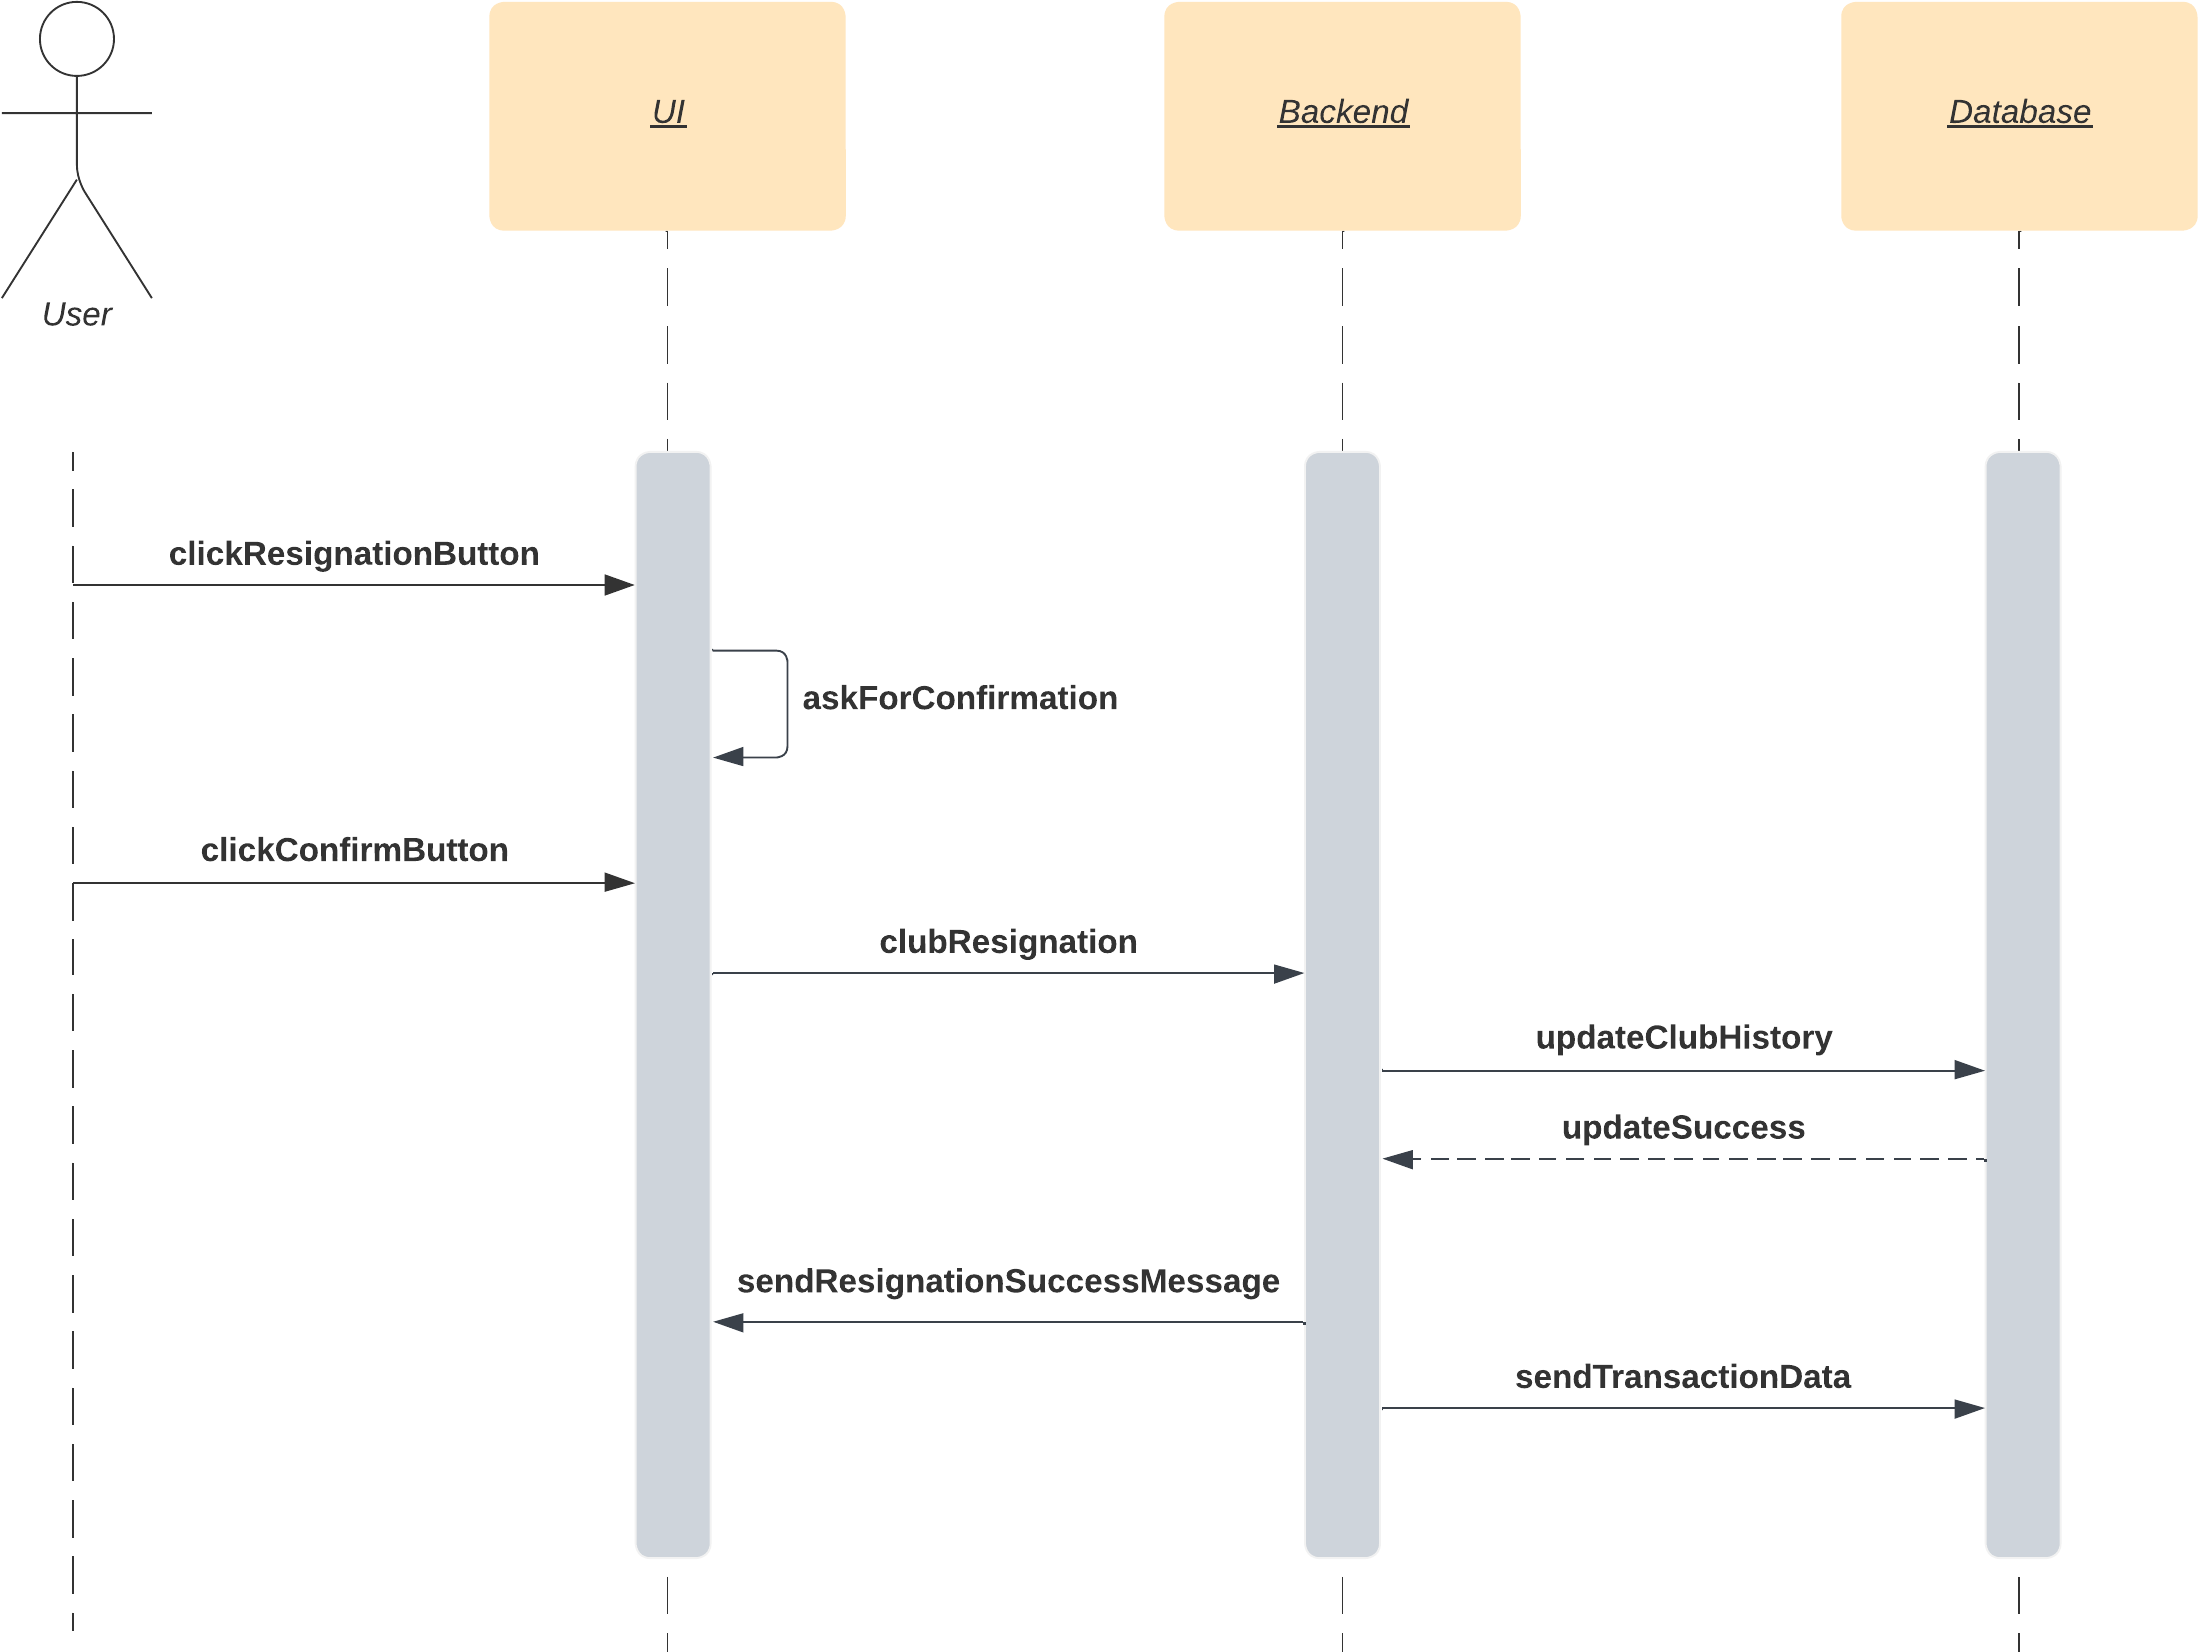
\includegraphics[width=15cm]{./clubregis.png}}
    \caption{Club resignation}\label{fig:Club resignation}
  \end{figure}

Sequence diagram สำหรับแสดงการทำงานของระบบขณะที่ผู้ใช้งานทำการสมัครเข้าชมรม โดยหลังจากกดปุ่มสมัคร UI จะถามยืนยันการสมัคร หากผู้ใช้งานกดยืนยัน UI จะทำการส่งข้อมูลการใช้งานไปให้ Backend จัดเก็บใน Data base แล้วส่งข้อความยืนยันการสมัครไปให้ UI แสดงกับผู้ใช้งาน

\newpage

\subsection{Feed recommendation}

  \begin{figure}[!h]\centering
    \setlength{\fboxrule}{0.5mm} % can define this in the preamble
    \setlength{\fboxsep}{0.5cm}
    \fbox{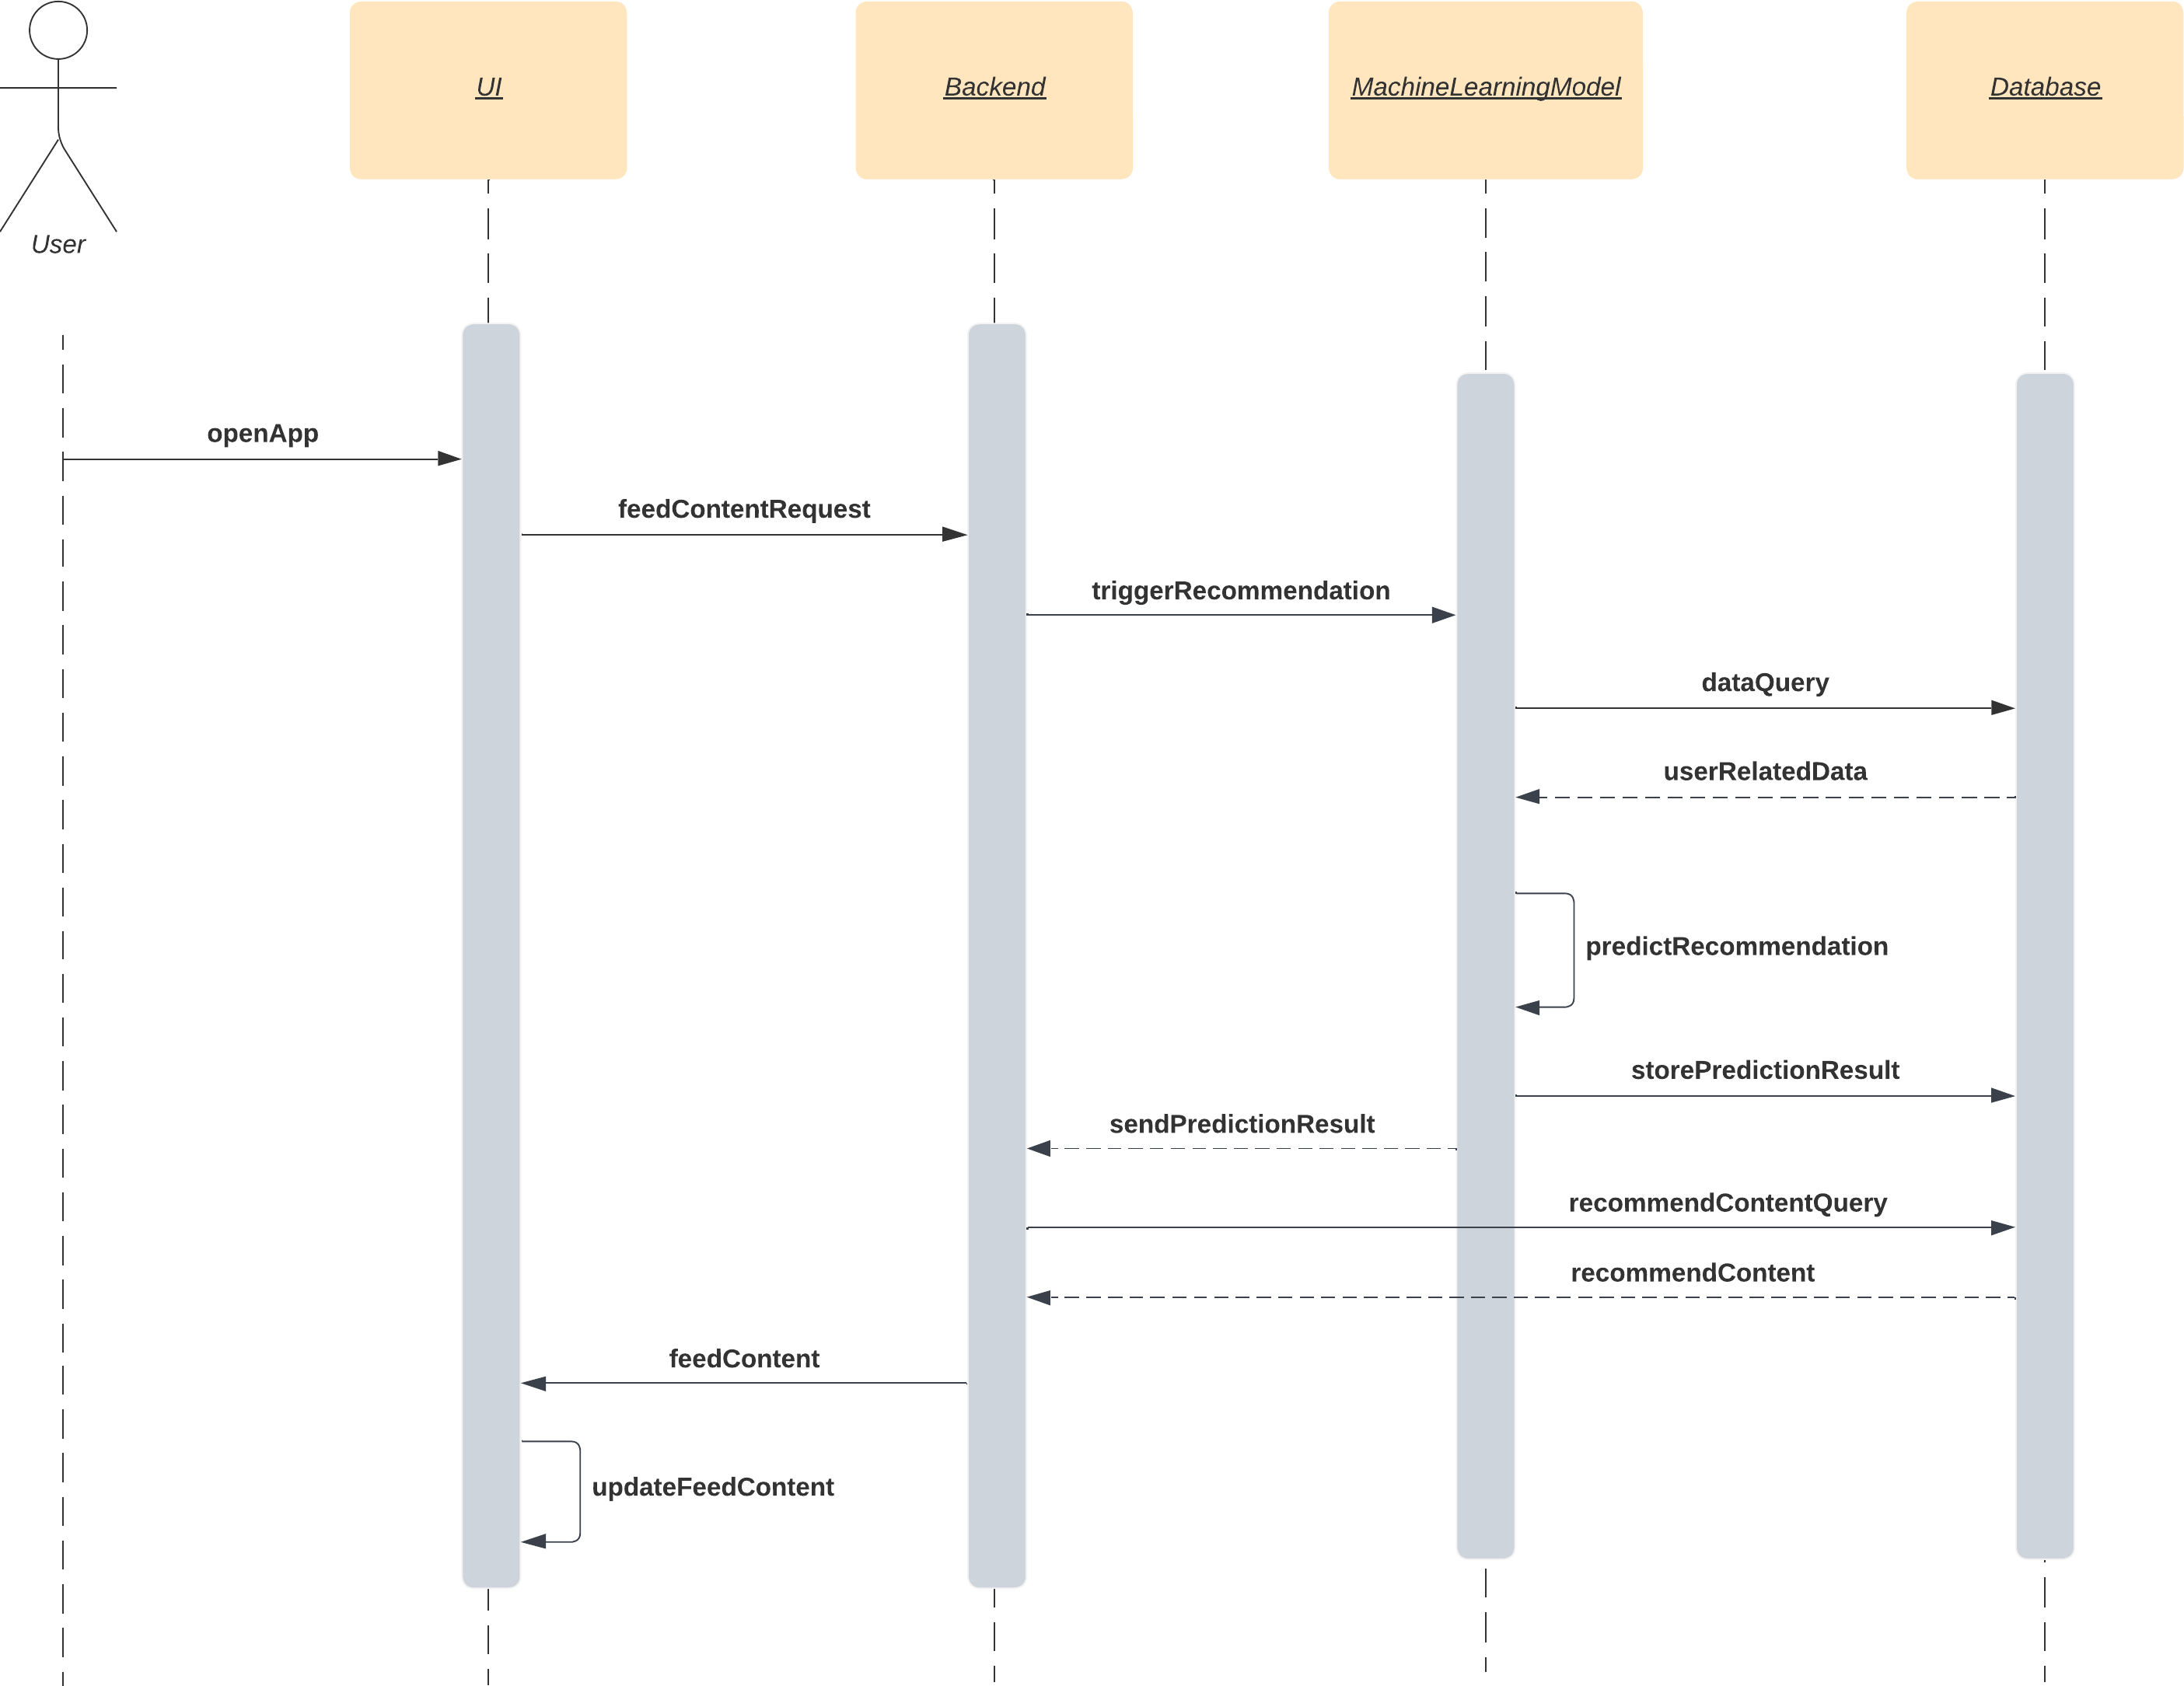
\includegraphics[width=15cm]{./Recommend.png}}
    \caption{Feed recommendation}\label{fig:Feed recommendation}
  \end{figure}

Sequence diagram สำหรับแสดงการทำงานของระบบเพื่อแนะนำกิจกรรมให้ผู้ใช้งาน โดยหลังจากเข้าแิปพลิเคชัน UI จะร้องขอเนื้อหาที่จะแนะนำไปยัง Backend เพื่อไปสั่งระบบ Machine learning Model เพื่อประมวลผลคำแนะนำซึ่งดึงข้อมูลที่เก็บไว้จาก Database มาประมวลผล ซึ่งจะส่งทั้งคำแนะนำกลับไปหา ทั้ง Backend เพื่อส่งคำแนะนำไปหาผู้ใช้งาน และ Data base เพื่อเก็บผลคำแนะนำที่ประมวลมาได้ Backend สามารถเรียกคำแนะนำที่ถูกเก็บเอาไว้มาเพื่อแสดงแก่ผู้ใช้งานได้

\newpage

\subsection{Machine learning training}

  \begin{figure}[!h]\centering
    \setlength{\fboxrule}{0.5mm} % can define this in the preamble
    \setlength{\fboxsep}{0.5cm}
    \fbox{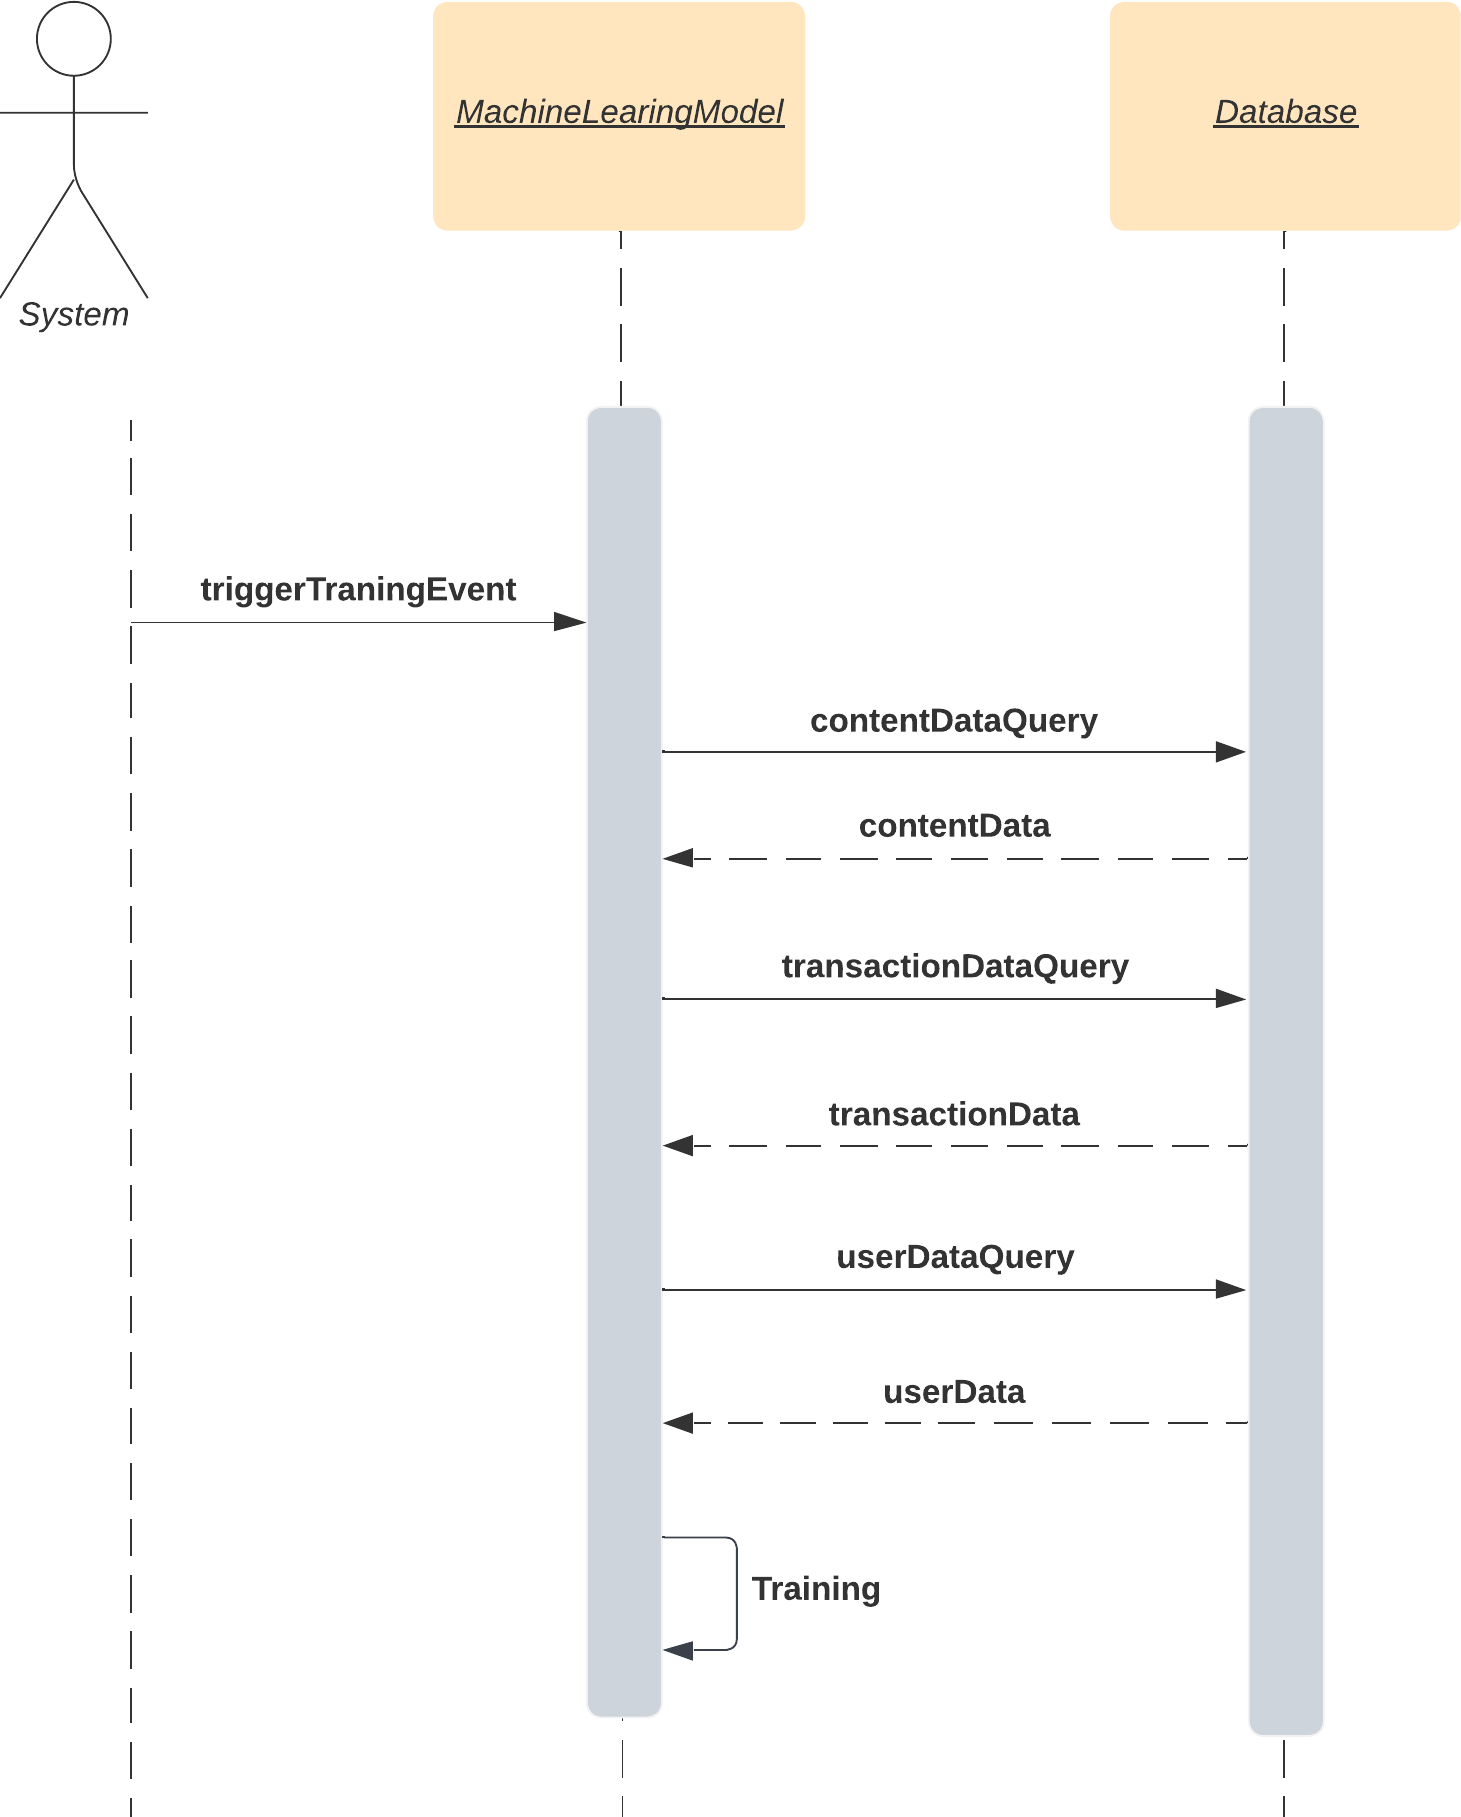
\includegraphics[width=15cm]{./Machinelearning.png}}
    \caption{Machine learning training}\label{fig:Machine learning training}
  \end{figure}

Sequence diagram สำหรับแสดงการทำงานของระบบในขณะที่ Train Machine Learning Model ใหม่ โดย Machine Learning Model จะดึงข้อมูลกิจกรรมและการใช้งานมาจาก Data base แล้วทำการ Train ตัวเอง

\newpage

\section{Database Model}

  \begin{figure}[!h]\centering
    \setlength{\fboxrule}{0.5mm} % can define this in the preamble
    \setlength{\fboxsep}{0.5cm}
    \fbox{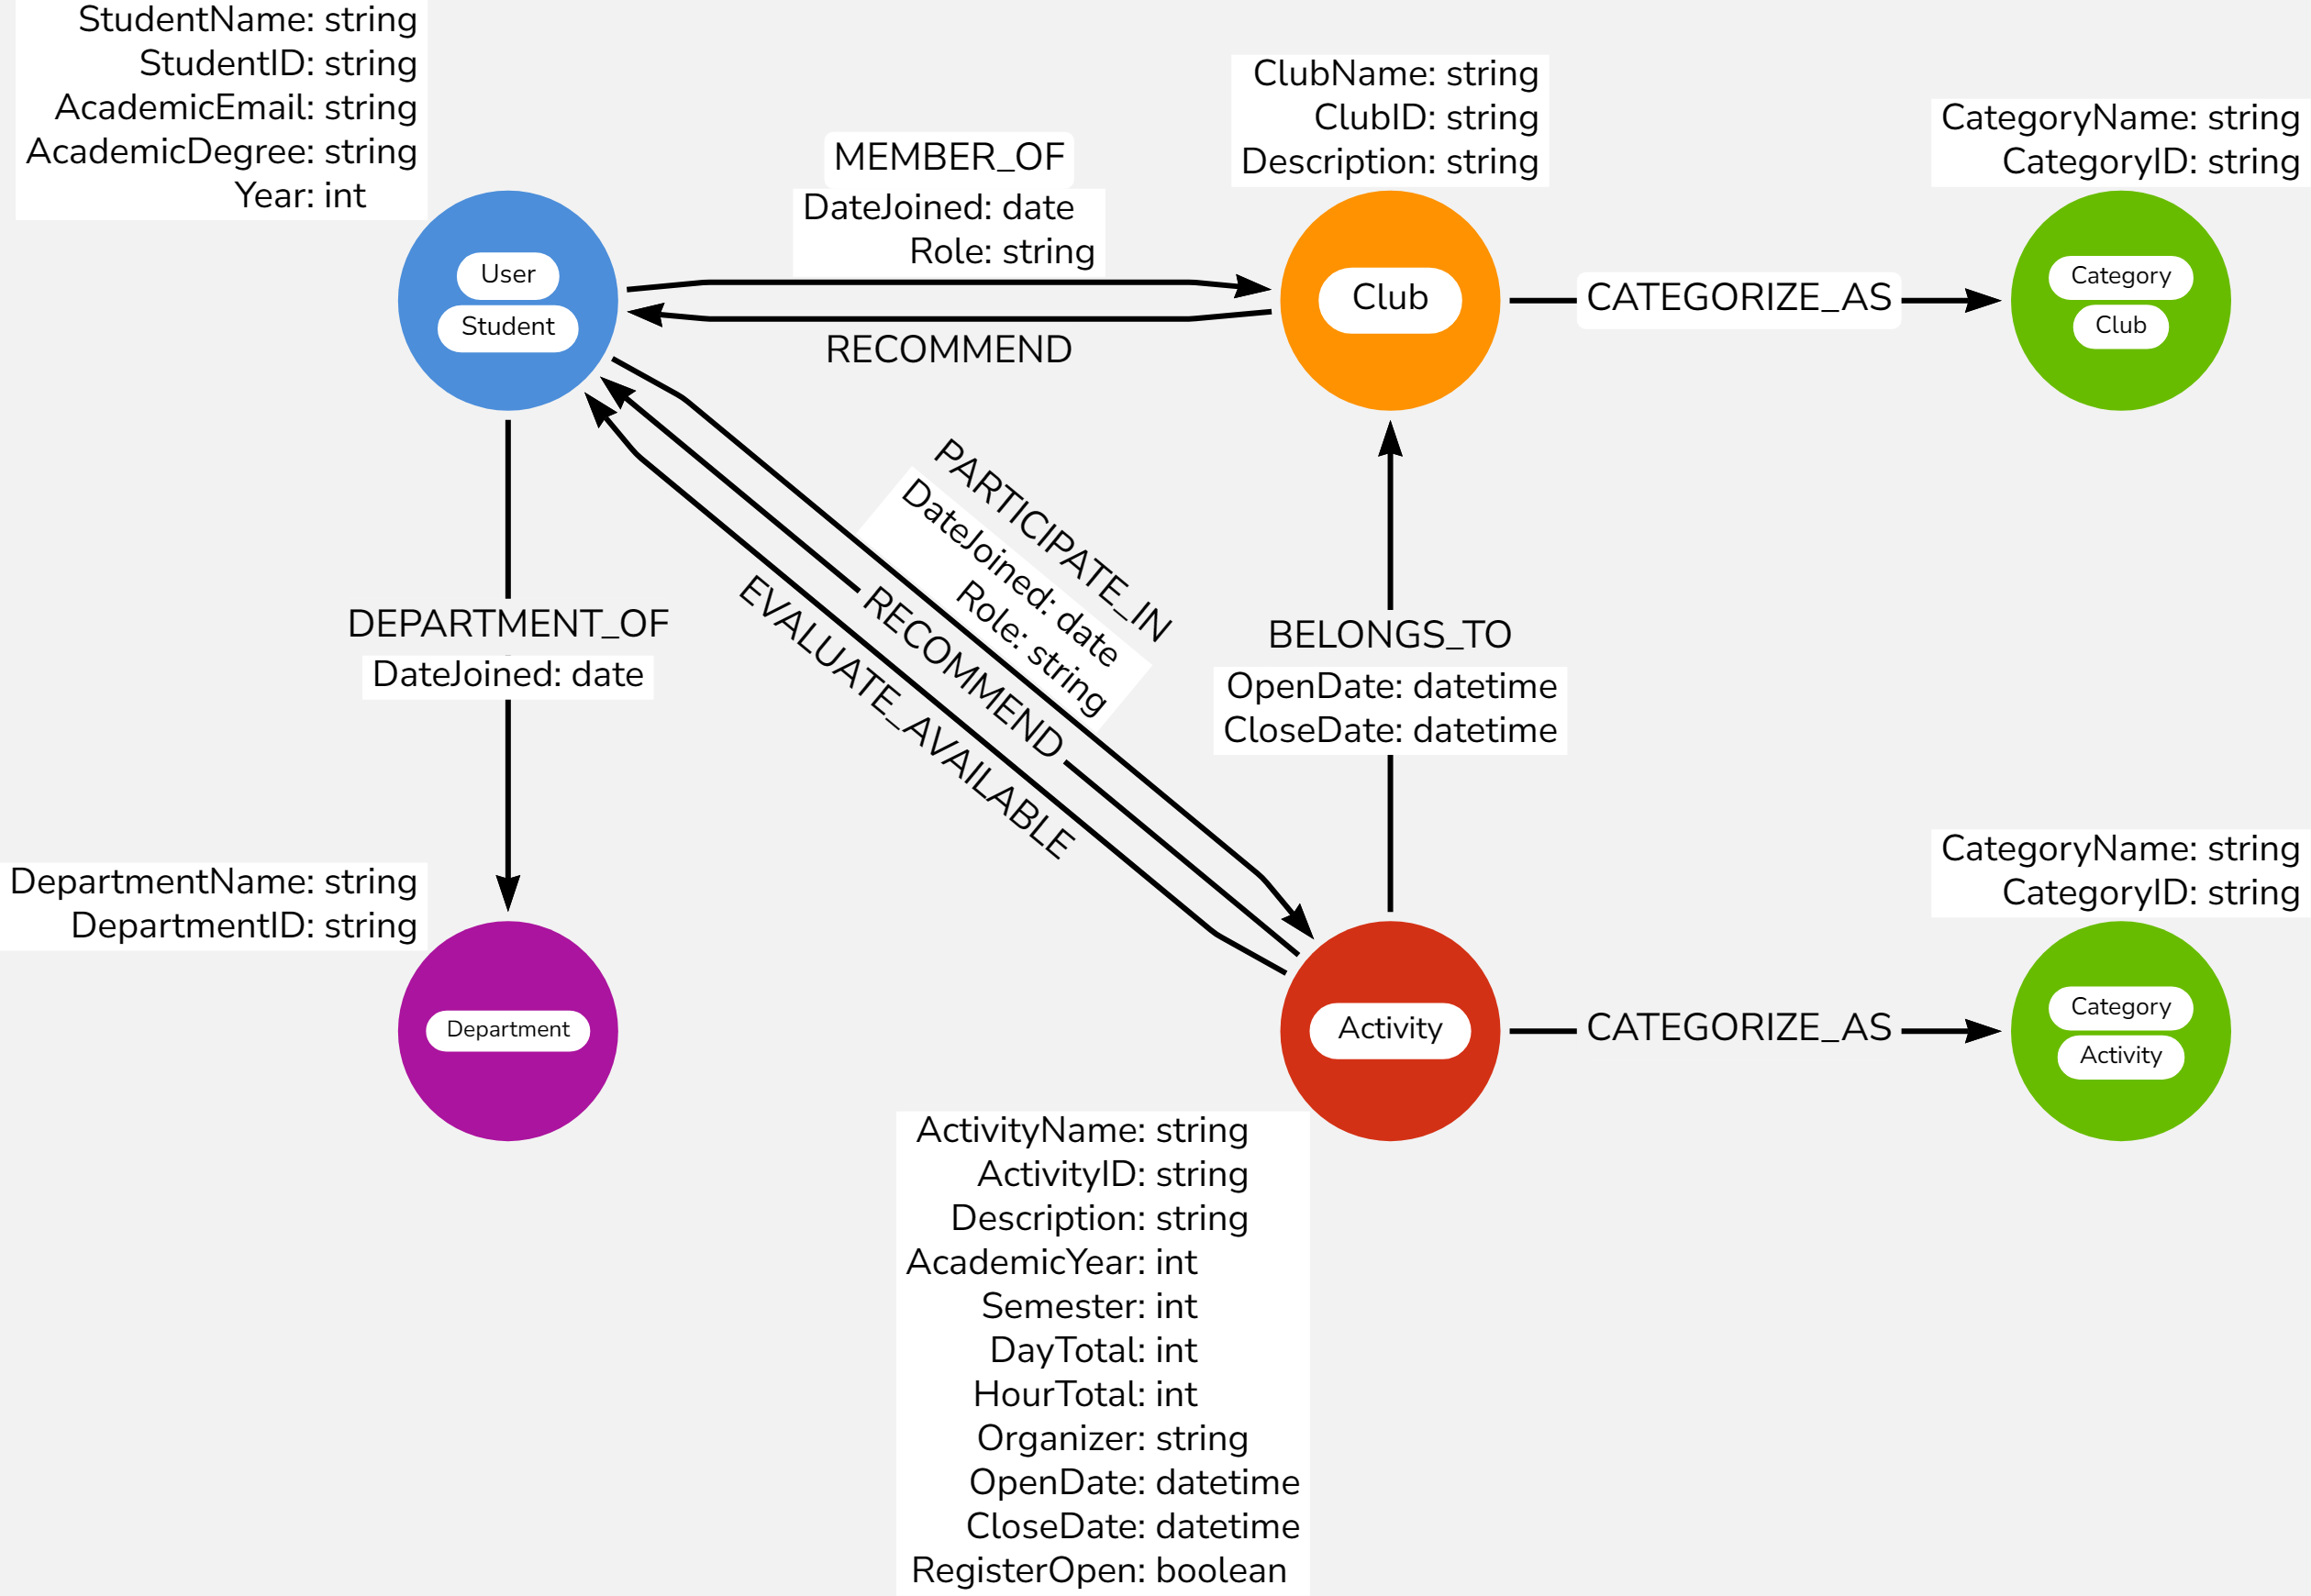
\includegraphics[width=15cm]{./DB.png}}
    \caption{Database Model}\label{fig:Database Model}
  \end{figure}

\makeatletter
\g@addto@macro{\UrlBreaks}{\UrlOrds}
\makeatother

\bibliographystyle{kmutt}
\bibliography{string,cpe}

\end{document}